% Options for packages loaded elsewhere
\PassOptionsToPackage{unicode}{hyperref}
\PassOptionsToPackage{hyphens}{url}
%
\documentclass[
]{book}
\usepackage{lmodern}
\usepackage{amssymb,amsmath}
\usepackage{ifxetex,ifluatex}
\ifnum 0\ifxetex 1\fi\ifluatex 1\fi=0 % if pdftex
  \usepackage[T1]{fontenc}
  \usepackage[utf8]{inputenc}
  \usepackage{textcomp} % provide euro and other symbols
\else % if luatex or xetex
  \usepackage{unicode-math}
  \defaultfontfeatures{Scale=MatchLowercase}
  \defaultfontfeatures[\rmfamily]{Ligatures=TeX,Scale=1}
\fi
% Use upquote if available, for straight quotes in verbatim environments
\IfFileExists{upquote.sty}{\usepackage{upquote}}{}
\IfFileExists{microtype.sty}{% use microtype if available
  \usepackage[]{microtype}
  \UseMicrotypeSet[protrusion]{basicmath} % disable protrusion for tt fonts
}{}
\makeatletter
\@ifundefined{KOMAClassName}{% if non-KOMA class
  \IfFileExists{parskip.sty}{%
    \usepackage{parskip}
  }{% else
    \setlength{\parindent}{0pt}
    \setlength{\parskip}{6pt plus 2pt minus 1pt}}
}{% if KOMA class
  \KOMAoptions{parskip=half}}
\makeatother
\usepackage{xcolor}
\IfFileExists{xurl.sty}{\usepackage{xurl}}{} % add URL line breaks if available
\IfFileExists{bookmark.sty}{\usepackage{bookmark}}{\usepackage{hyperref}}
\hypersetup{
  pdftitle={R Programming in Plain English},
  pdfauthor={Taylor Rodgers},
  hidelinks,
  pdfcreator={LaTeX via pandoc}}
\urlstyle{same} % disable monospaced font for URLs
\usepackage{color}
\usepackage{fancyvrb}
\newcommand{\VerbBar}{|}
\newcommand{\VERB}{\Verb[commandchars=\\\{\}]}
\DefineVerbatimEnvironment{Highlighting}{Verbatim}{commandchars=\\\{\}}
% Add ',fontsize=\small' for more characters per line
\usepackage{framed}
\definecolor{shadecolor}{RGB}{248,248,248}
\newenvironment{Shaded}{\begin{snugshade}}{\end{snugshade}}
\newcommand{\AlertTok}[1]{\textcolor[rgb]{0.94,0.16,0.16}{#1}}
\newcommand{\AnnotationTok}[1]{\textcolor[rgb]{0.56,0.35,0.01}{\textbf{\textit{#1}}}}
\newcommand{\AttributeTok}[1]{\textcolor[rgb]{0.77,0.63,0.00}{#1}}
\newcommand{\BaseNTok}[1]{\textcolor[rgb]{0.00,0.00,0.81}{#1}}
\newcommand{\BuiltInTok}[1]{#1}
\newcommand{\CharTok}[1]{\textcolor[rgb]{0.31,0.60,0.02}{#1}}
\newcommand{\CommentTok}[1]{\textcolor[rgb]{0.56,0.35,0.01}{\textit{#1}}}
\newcommand{\CommentVarTok}[1]{\textcolor[rgb]{0.56,0.35,0.01}{\textbf{\textit{#1}}}}
\newcommand{\ConstantTok}[1]{\textcolor[rgb]{0.00,0.00,0.00}{#1}}
\newcommand{\ControlFlowTok}[1]{\textcolor[rgb]{0.13,0.29,0.53}{\textbf{#1}}}
\newcommand{\DataTypeTok}[1]{\textcolor[rgb]{0.13,0.29,0.53}{#1}}
\newcommand{\DecValTok}[1]{\textcolor[rgb]{0.00,0.00,0.81}{#1}}
\newcommand{\DocumentationTok}[1]{\textcolor[rgb]{0.56,0.35,0.01}{\textbf{\textit{#1}}}}
\newcommand{\ErrorTok}[1]{\textcolor[rgb]{0.64,0.00,0.00}{\textbf{#1}}}
\newcommand{\ExtensionTok}[1]{#1}
\newcommand{\FloatTok}[1]{\textcolor[rgb]{0.00,0.00,0.81}{#1}}
\newcommand{\FunctionTok}[1]{\textcolor[rgb]{0.00,0.00,0.00}{#1}}
\newcommand{\ImportTok}[1]{#1}
\newcommand{\InformationTok}[1]{\textcolor[rgb]{0.56,0.35,0.01}{\textbf{\textit{#1}}}}
\newcommand{\KeywordTok}[1]{\textcolor[rgb]{0.13,0.29,0.53}{\textbf{#1}}}
\newcommand{\NormalTok}[1]{#1}
\newcommand{\OperatorTok}[1]{\textcolor[rgb]{0.81,0.36,0.00}{\textbf{#1}}}
\newcommand{\OtherTok}[1]{\textcolor[rgb]{0.56,0.35,0.01}{#1}}
\newcommand{\PreprocessorTok}[1]{\textcolor[rgb]{0.56,0.35,0.01}{\textit{#1}}}
\newcommand{\RegionMarkerTok}[1]{#1}
\newcommand{\SpecialCharTok}[1]{\textcolor[rgb]{0.00,0.00,0.00}{#1}}
\newcommand{\SpecialStringTok}[1]{\textcolor[rgb]{0.31,0.60,0.02}{#1}}
\newcommand{\StringTok}[1]{\textcolor[rgb]{0.31,0.60,0.02}{#1}}
\newcommand{\VariableTok}[1]{\textcolor[rgb]{0.00,0.00,0.00}{#1}}
\newcommand{\VerbatimStringTok}[1]{\textcolor[rgb]{0.31,0.60,0.02}{#1}}
\newcommand{\WarningTok}[1]{\textcolor[rgb]{0.56,0.35,0.01}{\textbf{\textit{#1}}}}
\usepackage{longtable,booktabs}
% Correct order of tables after \paragraph or \subparagraph
\usepackage{etoolbox}
\makeatletter
\patchcmd\longtable{\par}{\if@noskipsec\mbox{}\fi\par}{}{}
\makeatother
% Allow footnotes in longtable head/foot
\IfFileExists{footnotehyper.sty}{\usepackage{footnotehyper}}{\usepackage{footnote}}
\makesavenoteenv{longtable}
\usepackage{graphicx,grffile}
\makeatletter
\def\maxwidth{\ifdim\Gin@nat@width>\linewidth\linewidth\else\Gin@nat@width\fi}
\def\maxheight{\ifdim\Gin@nat@height>\textheight\textheight\else\Gin@nat@height\fi}
\makeatother
% Scale images if necessary, so that they will not overflow the page
% margins by default, and it is still possible to overwrite the defaults
% using explicit options in \includegraphics[width, height, ...]{}
\setkeys{Gin}{width=\maxwidth,height=\maxheight,keepaspectratio}
% Set default figure placement to htbp
\makeatletter
\def\fps@figure{htbp}
\makeatother
\setlength{\emergencystretch}{3em} % prevent overfull lines
\providecommand{\tightlist}{%
  \setlength{\itemsep}{0pt}\setlength{\parskip}{0pt}}
\setcounter{secnumdepth}{5}
\usepackage{booktabs}
\usepackage{amsthm}
\makeatletter
\def\thm@space@setup{%
  \thm@preskip=8pt plus 2pt minus 4pt
  \thm@postskip=\thm@preskip
}
\makeatother
\usepackage[]{natbib}
\bibliographystyle{plainnat}

\title{R Programming in Plain English}
\author{Taylor Rodgers}
\date{2021-04-03}

\begin{document}
\maketitle

{
\setcounter{tocdepth}{1}
\tableofcontents
}
\hypertarget{about-this-book}{%
\chapter{About This Book}\label{about-this-book}}

I never liked most programming books. The same with most programming courses. The reason is that many of them assume you already have a programming background.

That assumption doesn't work well with the R programming language. It's unique because it's a \emph{statistical} programming language. That means the people often needing to learn it are researchers, statisticians, and data analysts -- not computer engineers.

That's why I wrote this book. I wanted to explain R programming to people who don't know how to program. I want to strip away all the bloated, technical jargon used in most texts and explain R programming ``in plain English.''

It's hard enough to learn statistics. The same for psychology, business, sociology, medicine, economics, marketing, or whatever you were crazy enough to devote the best years of your life to learning. We don't need the programming language we use to analyze our data to be as hard to learn as the subject itself.

\hypertarget{things-you-should-know-before-reading}{%
\section{Things You Should Know Before Reading}\label{things-you-should-know-before-reading}}

Since R is used mostly for statistics, you should know some statistics before reading this book. For example, I assume you know what a p-value is. The same for confidence intervals, regression analysis, and R-square.

That being said, this book would make a great companion piece to your first statistics class. If your book or professor references code to perform certain calculations, this will help you understand what it's doing.

With that out of the way, let's begin!

\hypertarget{whatisr}{%
\chapter{What is R Programming?}\label{whatisr}}

Before getting setup in R, you need to know what R programming is and what's so special about it.

R is a programming language built by statisticians for statistical analysis. It is well-suited towards running advanced analysis, building predictive models, machine learning, and even more routine data management.

R is \textbf{open source}. That means it's free. The people who developed it wanted to make it accessible to anyone. Since then, R has moved beyond its humble beginnings and developed into a full-blown community of developers.

Developers within the community contribute to the R language by developing packages. \textbf{Packages} contain functions that allow you to perform certain tasks.

What does that mean in plain English?

Imagine what it's like to move into a new apartment. It's usually empty when you first move in, but it has running water, a refrigerator, and place to stay warm. So it meets the basic criteria for living - food, water, and shelter.

That's similar to what \textbf{base R} provides. It meets the bare necessities to get started with statistical programming.

An R \textbf{package} is like the new furniture you bring into the apartment. It's the new coffee table and couch. It's the new coat of paint. All of those things that take an empty apartment and changes it to meet \emph{your} needs.

And that's what's so great about the R programming language. It has a lot of flexibility. If you find one package confusing or challenging, you can probably find an easier one to perform the same task. Or you can build your own functions instead. The only thing is you have to understand the basics first.

One of those basics is \textbf{objects}. We'll cover this extensively in another chapter, but R is an \emph{object-oriented} programming language. That means to succeed with it, you have to understand the object types and how they're used.

If that sounds overwhelming, don't worry. It's easier than you think. And focusing on these core components will go a long way to helping you succeed in R. As a matter of fact, I'd ``guesstimate'' that understanding R objects and packages will take care of 80\% of your needs with this language.

\hypertarget{is-r-the-best-statistical-programming-language}{%
\section{Is R the Best Statistical Programming Language?}\label{is-r-the-best-statistical-programming-language}}

That's a matter of debate and boy do people debate it. The nice thing about R is that it's free and open source and has a vibrant community that contributes to it. It's also meant for statistics. So much of the base functionality is well-suited towards statisticians and researchers alike.

The two big competitors to R are SAS and Python.

\textbf{SAS} is a statistical programming language built by a for-profit company. It's the opposite of open source, which means you have to pay money to use it. That's not necessarily a bad thing though. It means there's more rigorous quality testing because that's what people expect from software that costs money. R packages, on the other hand, may not be as rigorously quality checked. At least not those developed by the community and not the original developers.

The SAS Institute (the people who make SAS) have a lot of market power. They've been around for far longer and have ingrained themselves in academia and pharmaceutical research. Even though R and Python are the preferred choices for most newer companies and younger professionals, SAS has the advantage of being \textbf{legacy code}.

You're probably not familiar with that term if you haven't ever programmed before. What that means is that even if R and Python were better alternatives to SAS, it would cost an organization a lot of money and time to have its programmers go back and re-write all their automated, enterprise-wide code.

Personally, I'm actually a fan of SAS. I took it in my grad program and enjoyed its clean structure. Unlike R, which has so many packages and various ways to do the same things, SAS has the benefit of simplicity and clean documentation. That's nice when you are already forcing yourself to learn statistics and don't want to further stress yourself figuring out a programming language.

\textbf{Python} is an interesting competitor of R. It's interesting because it wasn't built for statistical programming. Like R, it's open source and that has led to data scientists building packages that make statistical programming possible.

Python is probably more popular with data scientists than researchers and statisticians. Since data scientists are often joined at the hip with computer programmers, it naturally lends itself more to that work.

I once worked with a company that ran all of its ETL (extract, transform, and load) processes off of Python. Since the data engineers and architects already used Python for that purpose, it wasn't difficult for them to learn to use it for data science as well.

Is Python better than R? I don't know because I haven't programmed much in Python. In my opinion, R is easier to learn for people who've already programmed in SQL, since it has a more direct syntax. Other people say that Python is easier to learn for programming newbies because it's written more like the English language. I didn't find that to be the case, myself.

If you want to develop automated, enterprise level solutions, I do think Python is a better choice. Mostly because it makes it easier for computer engineers to work with you. But if your goal is statistical analysis and reproducible research, R is better in my mind.

\hypertarget{things-to-remember}{%
\section{Things to Remember}\label{things-to-remember}}

\begin{itemize}
\tightlist
\item
  R programming is a free and allows for advanced statistical programming
\item
  R is managed by a community of developers, who contribute to its growth through packages
\item
  You must understand object types to succeed with R
\end{itemize}

\hypertarget{setup}{%
\chapter{Getting Setup in R and RStudio}\label{setup}}

This chapter will tell you how to download \textbf{R} and \textbf{RStudio}. It will also explain the differences between these two tools and how to navigate their user interfaces.

If you have already setup these two tools, feel free to skip ahead to the next chapter. However, if you're still unsure of how to navigate the tools, you may find certain sections useful.

\hypertarget{how-to-download-r}{%
\section{How to Download R}\label{how-to-download-r}}

To download R, go to this website: \url{https://www.r-project.org/}

You will then have to go through a series of options and screens to download R. Don't worry. I'll explain each of them along the way.

First, you'll select the ``download R'' link in the first paragraph.

\begin{center}
\includegraphics[width=0.5\linewidth]{1.1_R_Download} \end{center}

Second, you'll select a CRAN mirror. Select the one that's closest to you. For example, I live in Lawrence, Kansas. That conveniently has a CRAN mirror in my own city. If you live in Melbourne, Australia, you'll select the mirror hosted by the University of Melbourne.

\begin{center}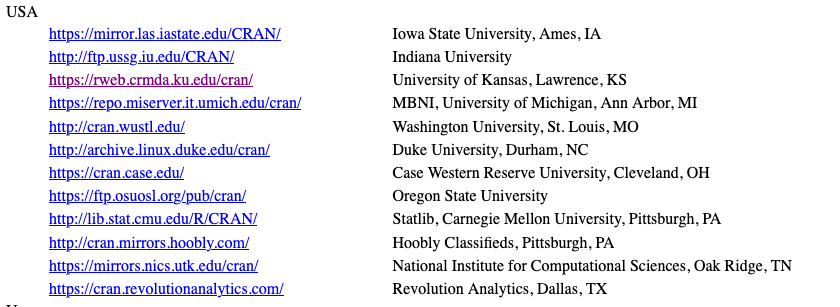
\includegraphics[width=0.75\linewidth]{1.2_CRAN_Selection} \end{center}

Don't worry. There's not much difference to the user in these mirrors. It simply helps optimize your ability to download packages from a nearby source, rather than from some other country in the world. This isn't a big deal for a small time programmer or researcher, but it's beneficial for large scale operations to carefully choose their mirror.

Third, you'll select the option for your operating system:

\begin{center}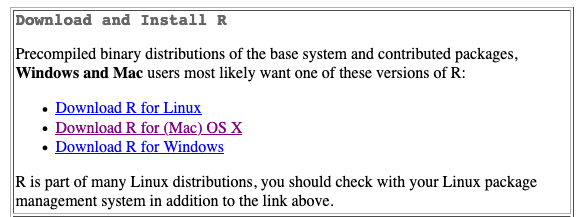
\includegraphics[width=0.65\linewidth]{1.3_Download_and_Install} \end{center}

That will take you to a page where you can select the latest release:

\begin{center}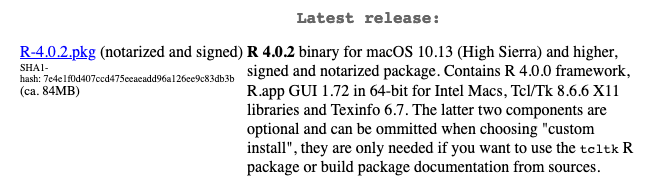
\includegraphics[width=0.75\linewidth]{1.4_Download} \end{center}

Download and install the latest release.

\hypertarget{understanding-base-rs-user-interface}{%
\section{Understanding Base R's User Interface}\label{understanding-base-rs-user-interface}}

I won't focus too much on the R interface. We won't use it much in this book. We'll be using RStudio (more on that in a bit). However, go ahead and open up R. If you have a Mac, it will have this icon:

\begin{center}
\includegraphics[width=0.1\linewidth]{1.5_R_Logo} \end{center}

Once you open it, you should see the \textbf{R console}. The R console is where you type commands. You'll continue to use the console in RStudio later.

\begin{center}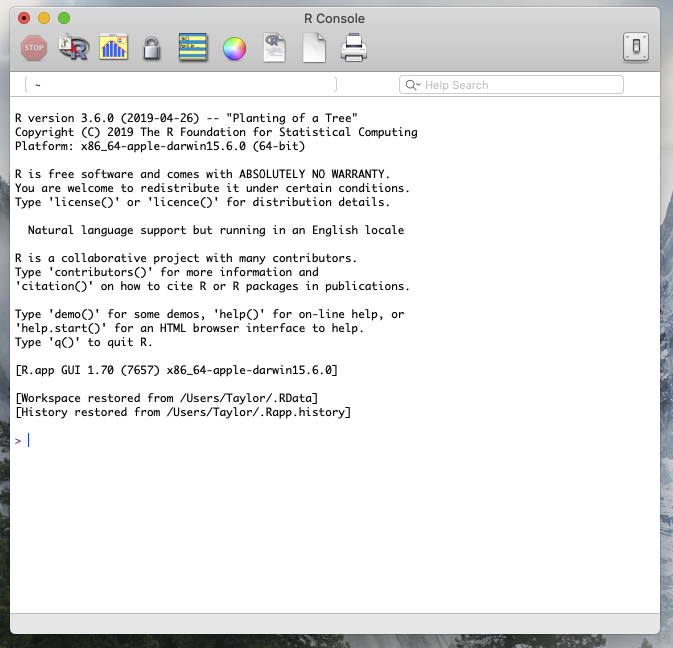
\includegraphics[width=0.75\linewidth]{1.6_R_Console} \end{center}

Go ahead and input \texttt{2*2} to get a feel for it. You can hit \textbf{Ctrl+Enter} on a Windows version and \textbf{Command+Enter} on a Mac OS to run the command.

\begin{Shaded}
\begin{Highlighting}[]
  \DecValTok{2}\OperatorTok{*}\DecValTok{2}
\end{Highlighting}
\end{Shaded}

\begin{verbatim}
## [1] 4
\end{verbatim}

As you notice, the R console doesn't allow you to go back and edit previously executed commands.

In order to save and edit a script, you'll need to create a document. A document in this context is basically just a text file that saves the code you want to reference later.

Go to the \textbf{File menu} and select \textbf{New Document}. You should have two windows afterwards like the screenshot below:

\begin{center}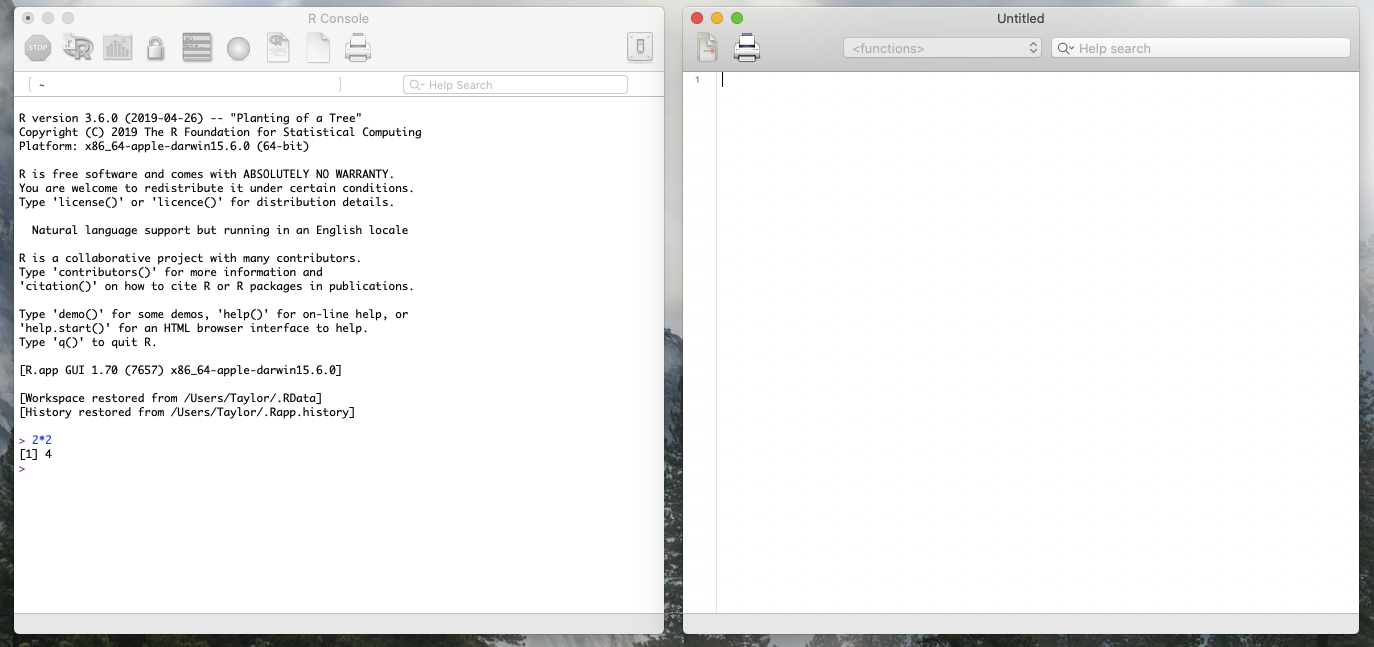
\includegraphics[width=0.75\linewidth]{1.7_New_Document} \end{center}

Go ahead and copy and paste this code into the document:

\begin{Shaded}
\begin{Highlighting}[]
  \KeywordTok{install.packages}\NormalTok{(}\StringTok{"faraway"}\NormalTok{)}
  \KeywordTok{library}\NormalTok{(faraway)}
  \KeywordTok{data}\NormalTok{(hprice)}
  \KeywordTok{head}\NormalTok{(hprice)}
\end{Highlighting}
\end{Shaded}

Highlight different parts of the code and hit \textbf{Command-Enter} or \textbf{Ctrl-Enter} and see how it interacts with the console. (It may ask you to re-select a CRAN mirror. Go ahead and re-select the one you used to download.)

\begin{center}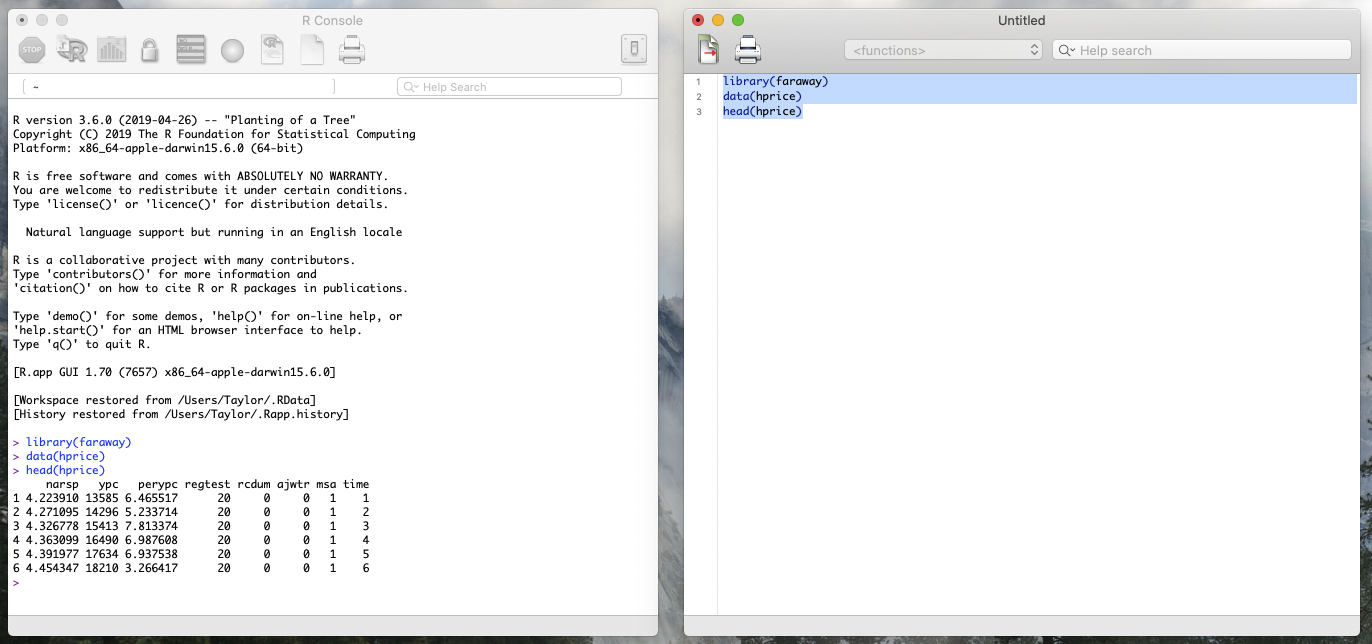
\includegraphics[width=0.75\linewidth]{1.8_Run_Code} \end{center}

Saving scripts this way allows you to modify your code and then re-execute it in the console.

We'll go into more detail about how to input and analyze data later.

Go ahead and close R for now. No need to save anything.

\hypertarget{limitations-of-r-base}{%
\section{Limitations of R Base}\label{limitations-of-r-base}}

The R console in the base version is a simple interface. Sometimes this is nice because you don't get overwhelmed with all the information displayed in RStudio, which we'll cover in a second. If you need to run a few calculations and know your data set well, this is a good setup.

The downside is that the console can't display large amounts of data.

If you look at the screen shot below, I attempted to review metadata from the US Census Bureau. As you can see, it's all squished together because the R console can't cleanly display it.

\begin{center}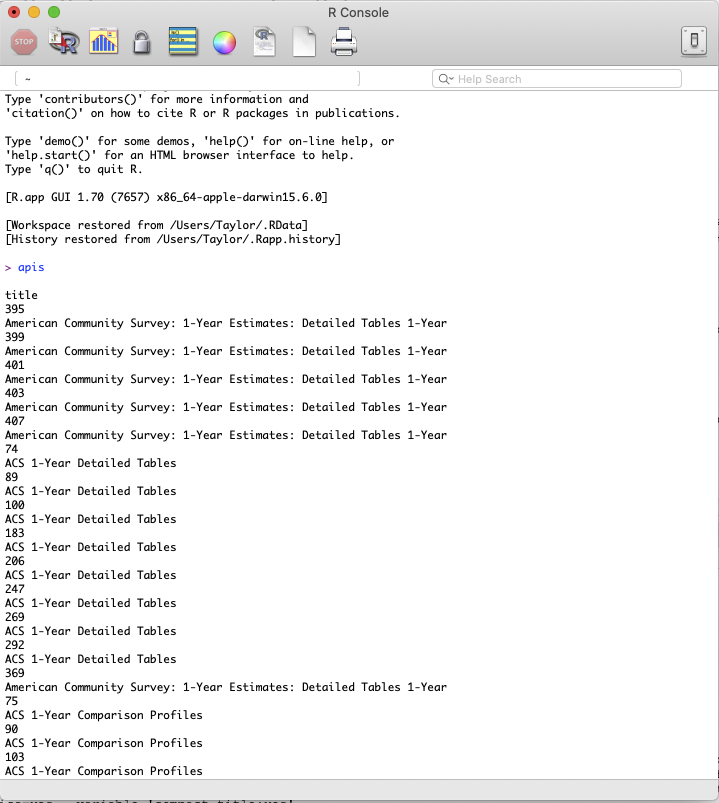
\includegraphics[width=0.5\linewidth]{1.9_RConsole_Census} \end{center}

In order to use the R console for further analysis, I'd have to find a different way to view this data I created.

That's where RStudio comes in handy.

\hypertarget{what-is-rstudio}{%
\section{What is RStudio?}\label{what-is-rstudio}}

If you don't already feel totally confused and overwhelmed with understanding R and R packages -- don't worry. I'm about to make things even more confusing by introducing you to RStudio!

\textbf{RStudio} is an IDE (integrated development environment) that allows more interactivity and for you to visually keep track of what you're doing.

In simpler words, it's a handy user interface for programming in R.

\begin{center}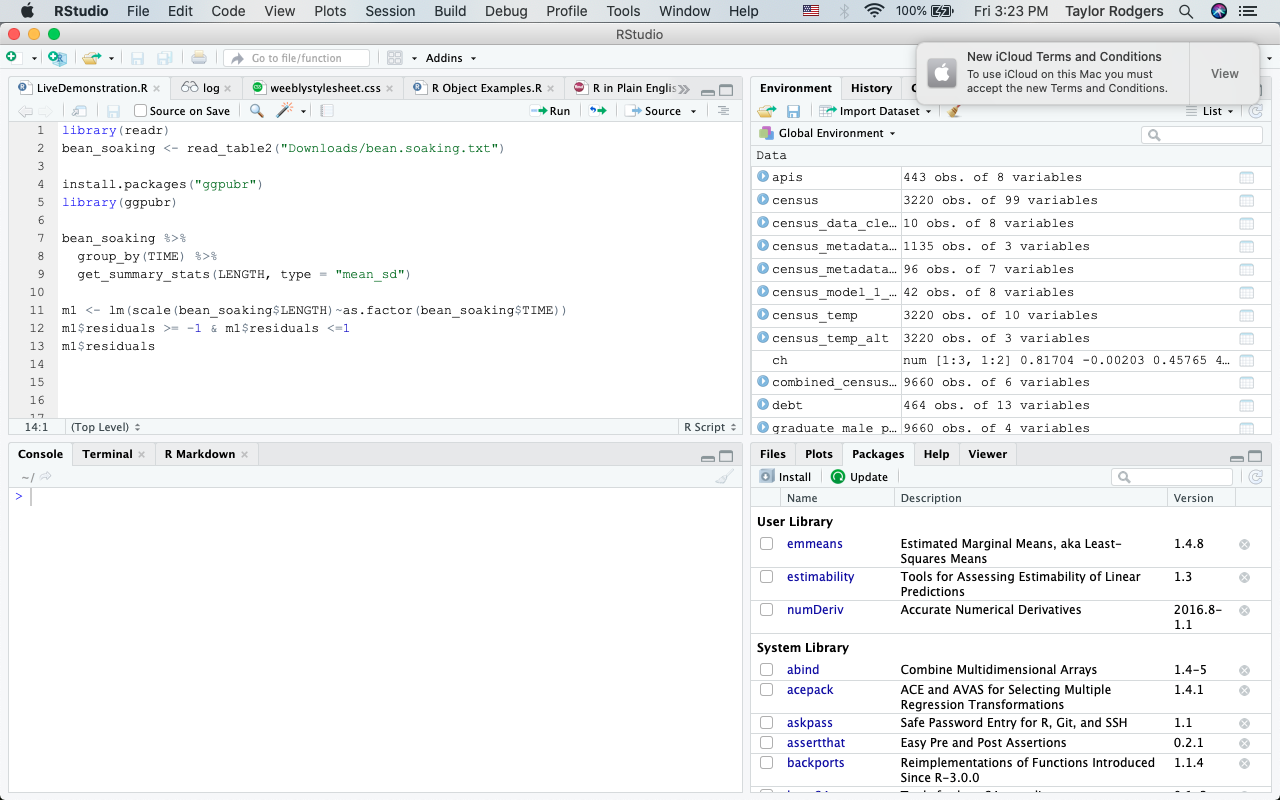
\includegraphics[width=0.75\linewidth]{1.10_RStudio} \end{center}

It's far easier to both get started and understand the R programming language by using RStudio. It makes importing data and packages easier. It also makes it easier to manage and visually review what data and packages you have loaded. And lastly, it's just plain nicer looking.

This book will primarily use RStudio for examples. I suggest downloading it to get the best use of my material.

\hypertarget{how-to-download-rstudio}{%
\section{How to Download RStudio}\label{how-to-download-rstudio}}

To download RStudio, go to this website: \url{https://rstudio.com/products/rstudio/download/}

Scroll down and you'll see a big blue button to download the latest version of RStudio.

\begin{center}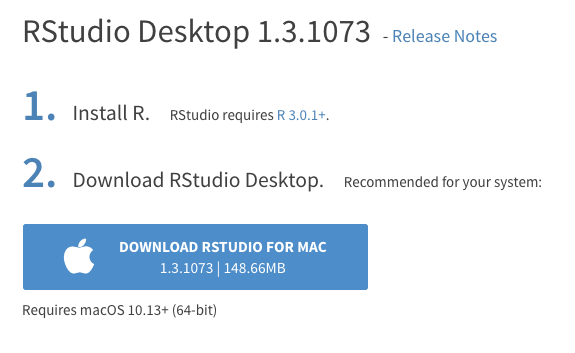
\includegraphics[width=0.5\linewidth]{1.11_RStudio_Download} \end{center}

You can tell that RStudio was designed for the end-user in mind by how painless it is to download compared to base R.

Go ahead and install it once the download finishes.

You'll see an icon like this appear in your applications folder. Go ahead and open it.

\begin{center}
\includegraphics[width=0.1\linewidth]{1.13.1_RStudio_Logo} \end{center}

\hypertarget{understanding-rstudio-interface}{%
\section{Understanding RStudio Interface}\label{understanding-rstudio-interface}}

The RStudio interface is broken up into four panes. The default pane setting has the following:

\begin{enumerate}
\def\labelenumi{\arabic{enumi}.}
\tightlist
\item
  Source
\item
  Console
\item
  Environment, History, and Connections
\item
  Files, Plots, Package, Help, and Viewer
\end{enumerate}

\begin{center}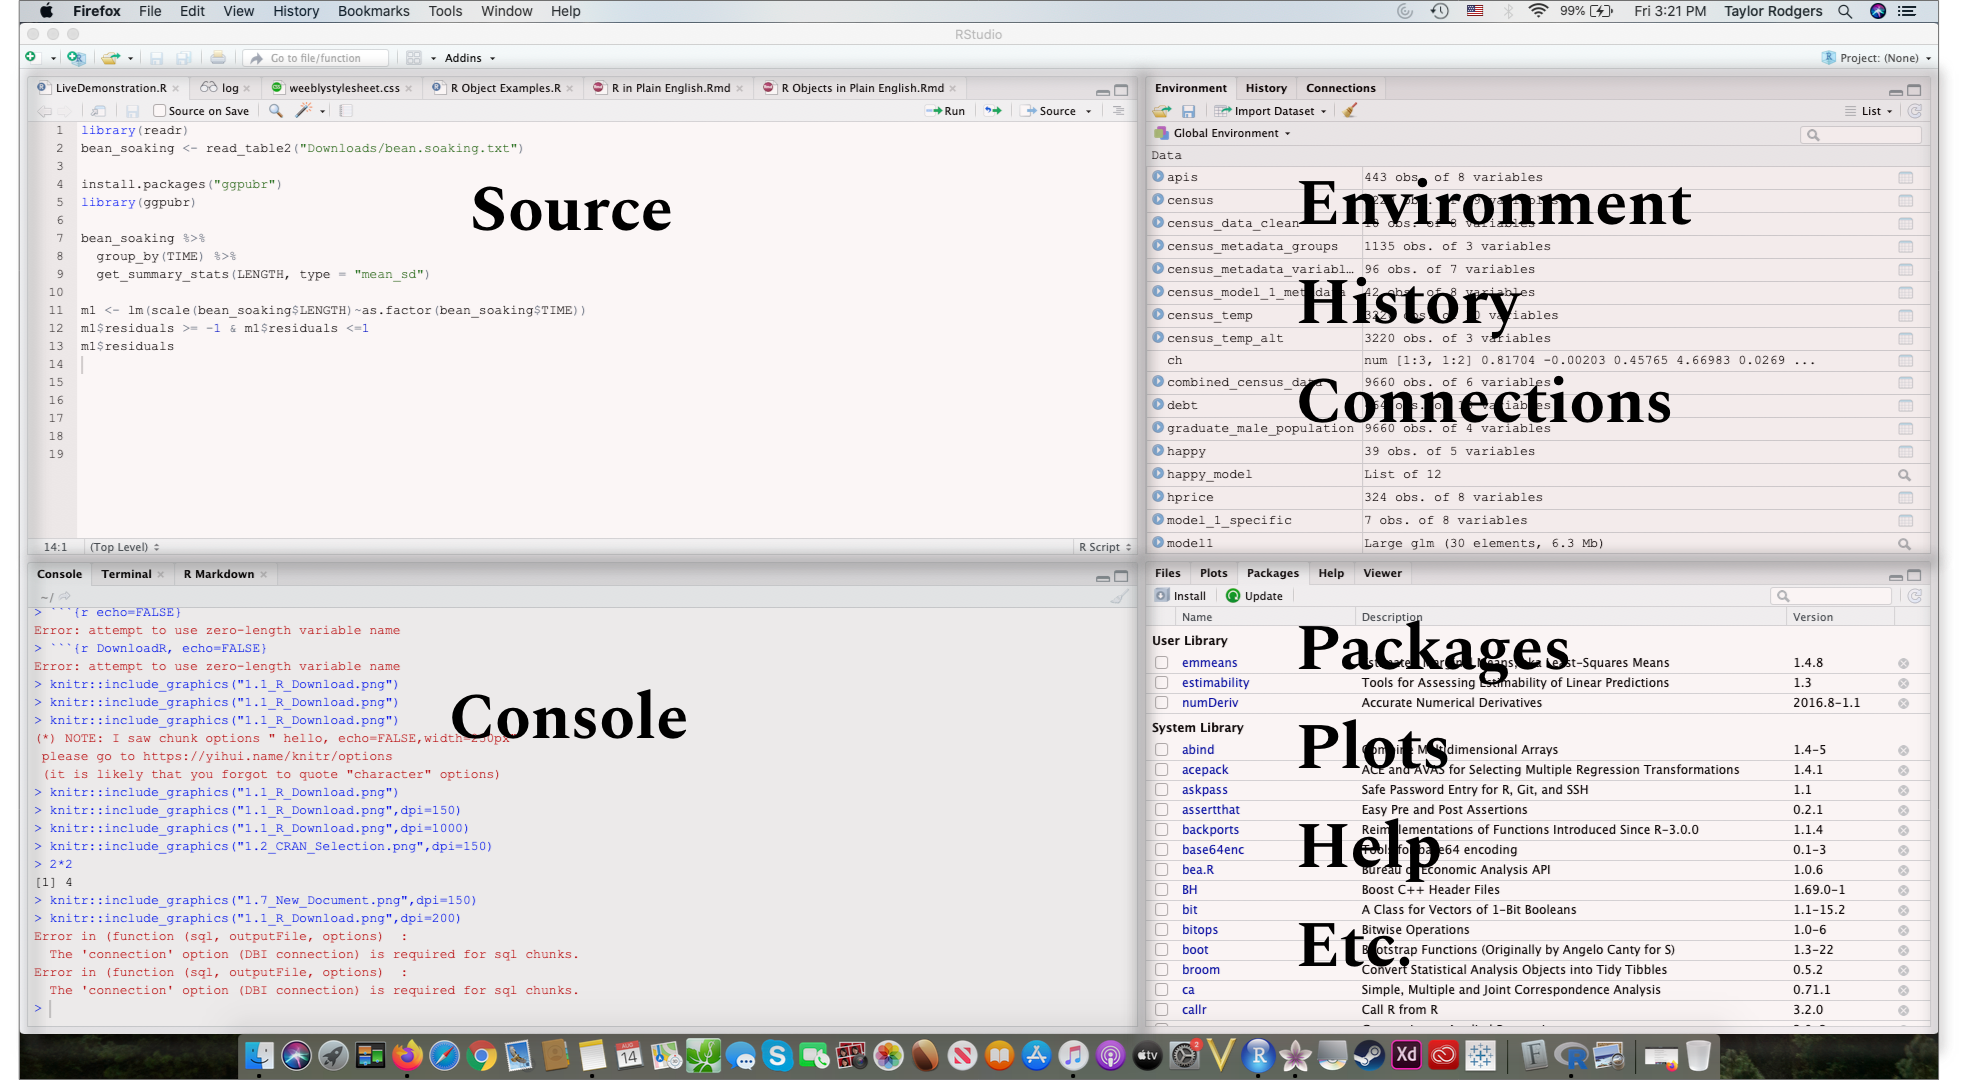
\includegraphics[width=0.75\linewidth]{1.12_RStudio_Labels} \end{center}

The \textbf{source} pane on the top left is a handy one.

\begin{center}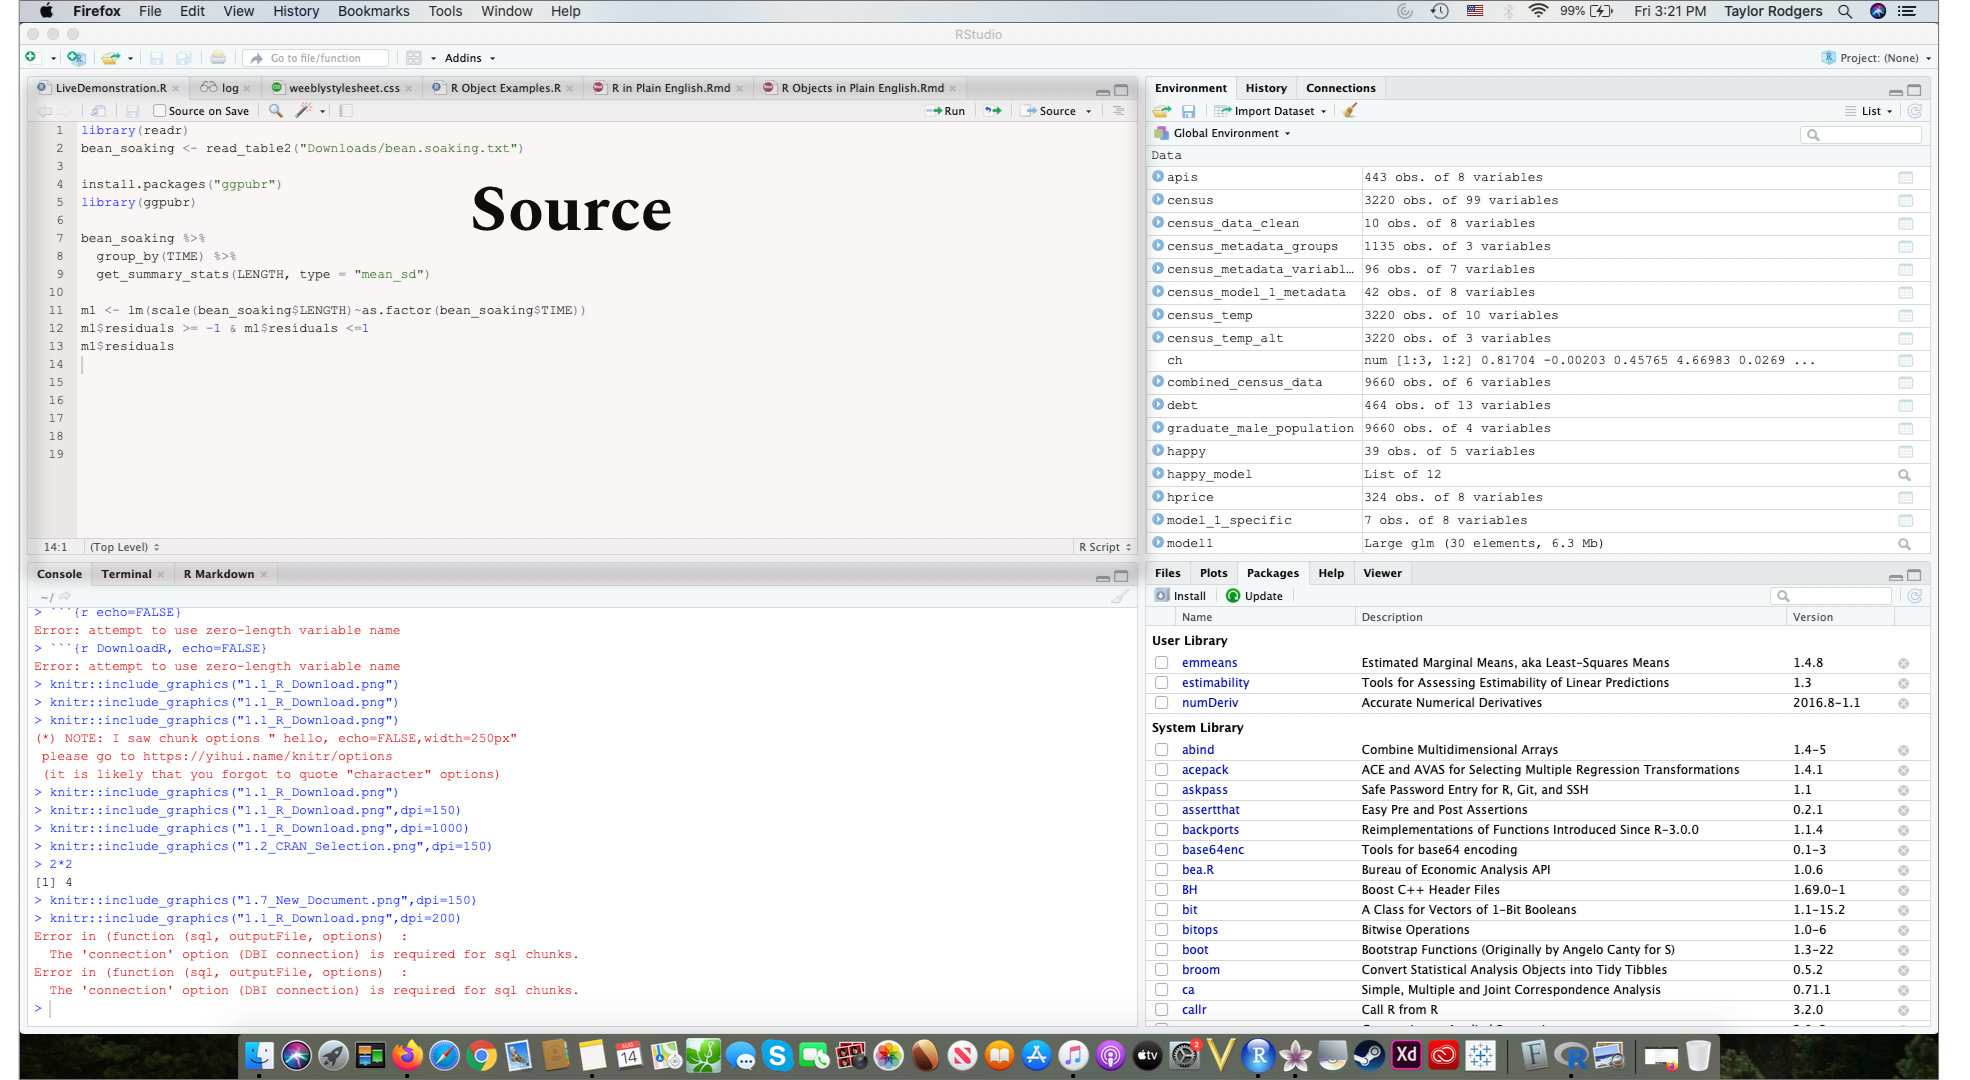
\includegraphics[width=0.75\linewidth]{1.13_RStudio_Source} \end{center}

This pane displays previously saved or new R scripts you wrote in the past.

\begin{center}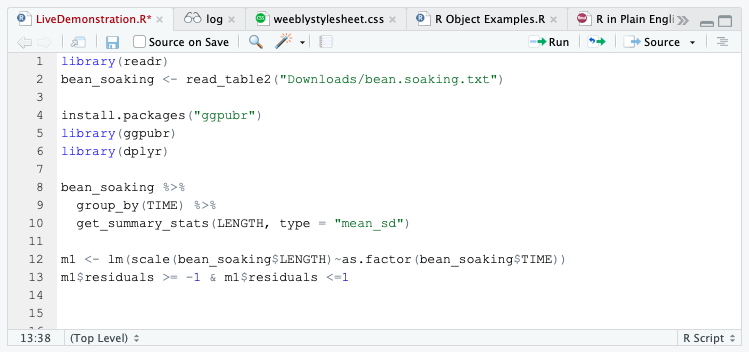
\includegraphics[width=0.75\linewidth]{1.14_Saved_Script} \end{center}

You may not be able to see this pane yet. Especially if you've never opened or saved a script before. To view the source pane, go to the top menu and click \textbf{File}, \textbf{New File}, and then \textbf{R Script}.

\begin{center}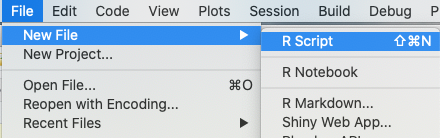
\includegraphics[width=0.65\linewidth]{1.14.1_New_R_Script} \end{center}

The source pane can also show loaded data sets as well.

\begin{center}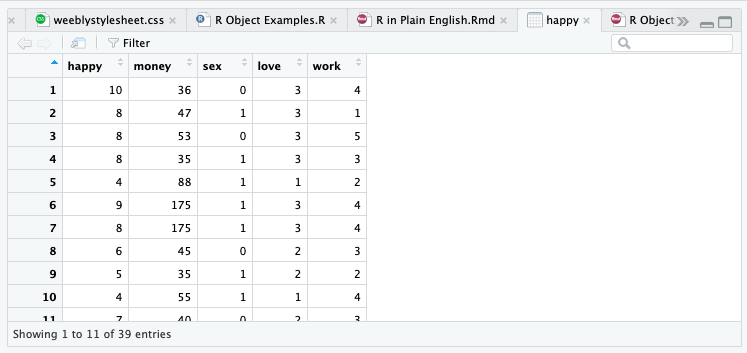
\includegraphics[width=0.75\linewidth]{1.15_Data_Set} \end{center}

If you recall, I said base R had a limitation if you want to review extremely large data sets. This is where RStudio really comes in handy. Down below is the same Census data set that I attempted to view earlier:

\begin{center}\includegraphics[width=0.75\linewidth]{1.16_API_List} \end{center}

And here is how it looked in base R:

\begin{center}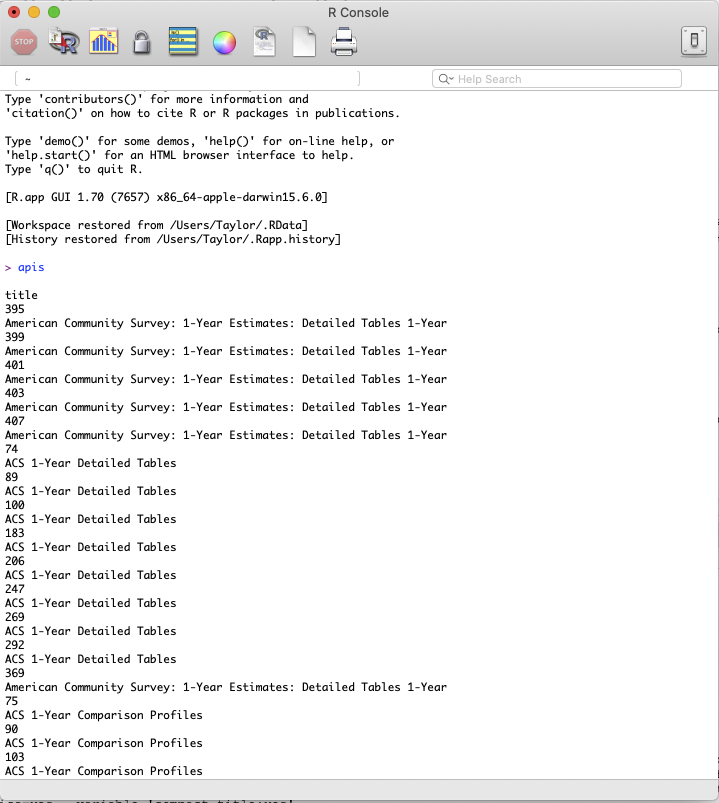
\includegraphics[width=0.75\linewidth]{1.9_RConsole_Census} \end{center}

The \textbf{console} pane on the bottom left is more or less the same as the base R console we reviewed earlier. It allows you to enter commands.

\begin{center}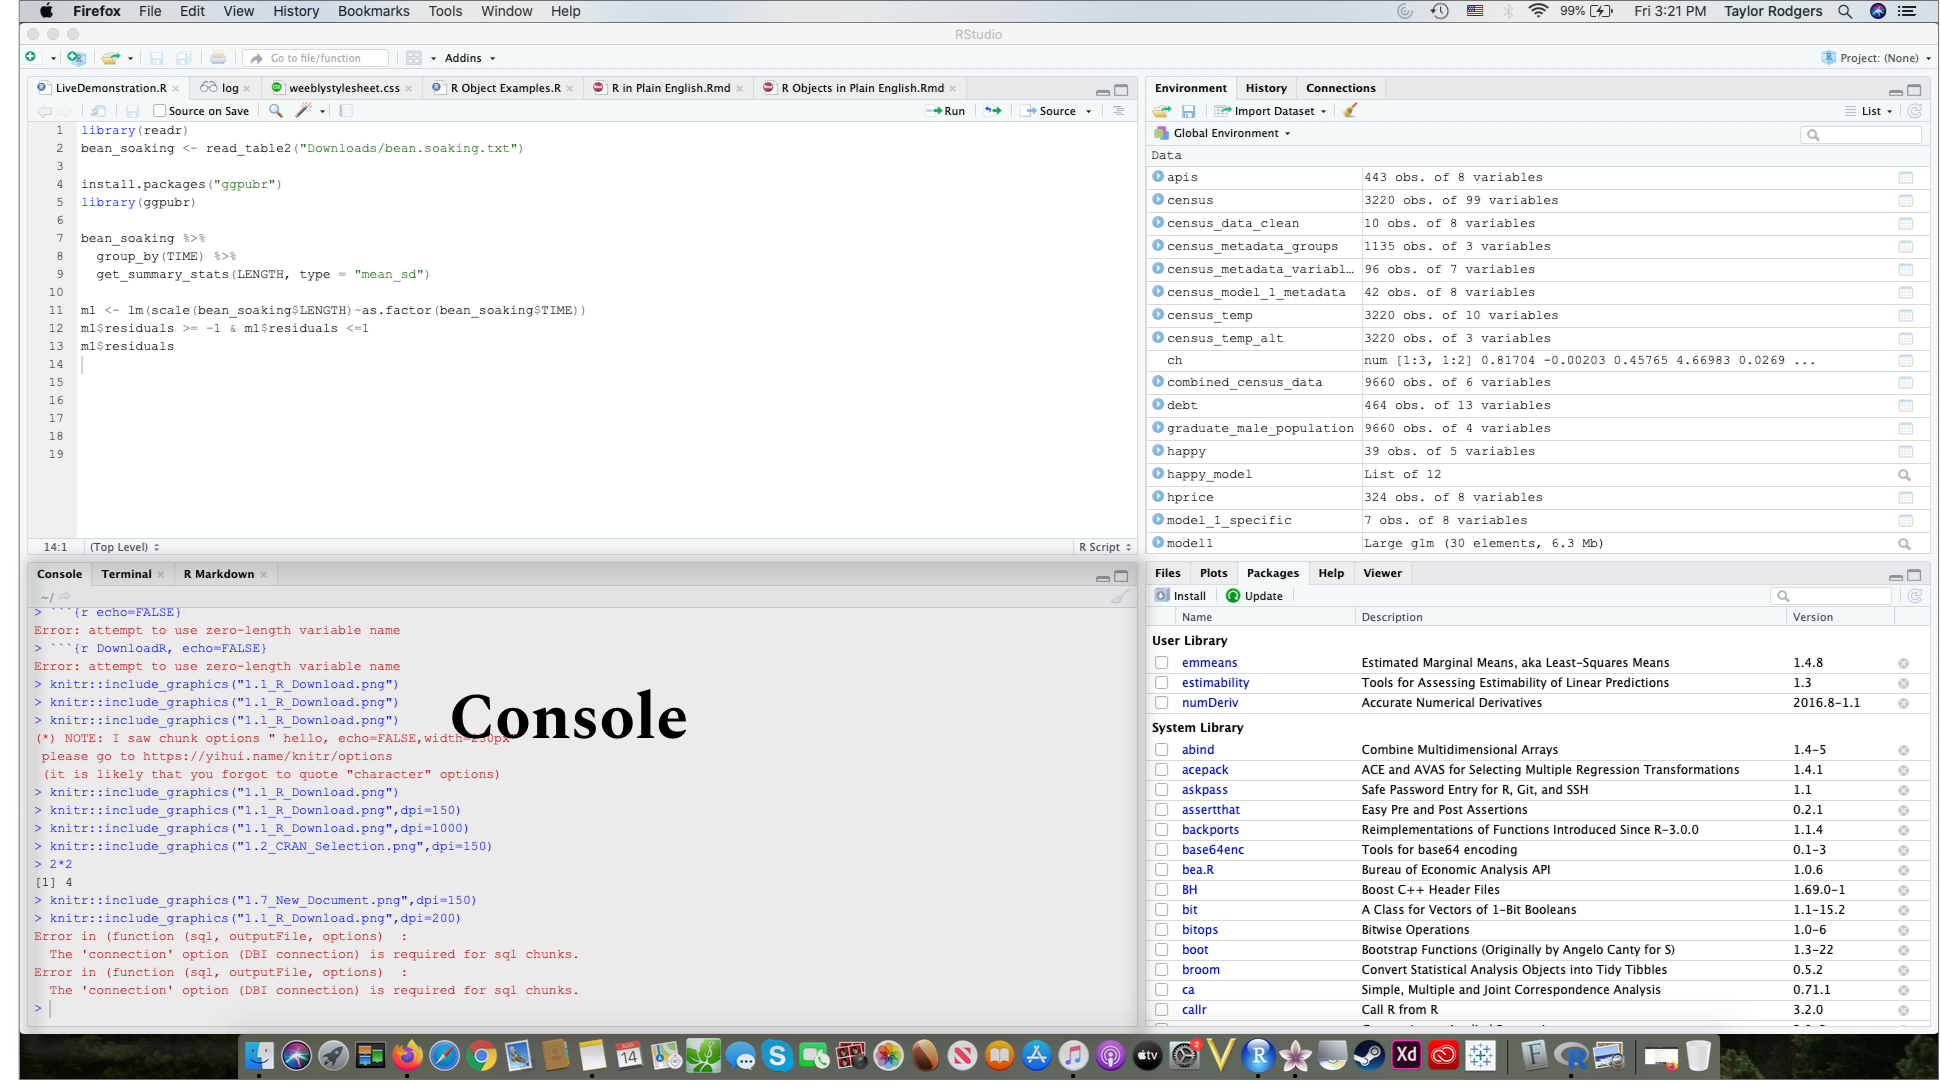
\includegraphics[width=0.75\linewidth]{1.17_RStudio_Console} \end{center}

However, you won't be able to save those commands as a script unless you write them in the source pane above. That's similar to what we did with base R and that new document.

\begin{center}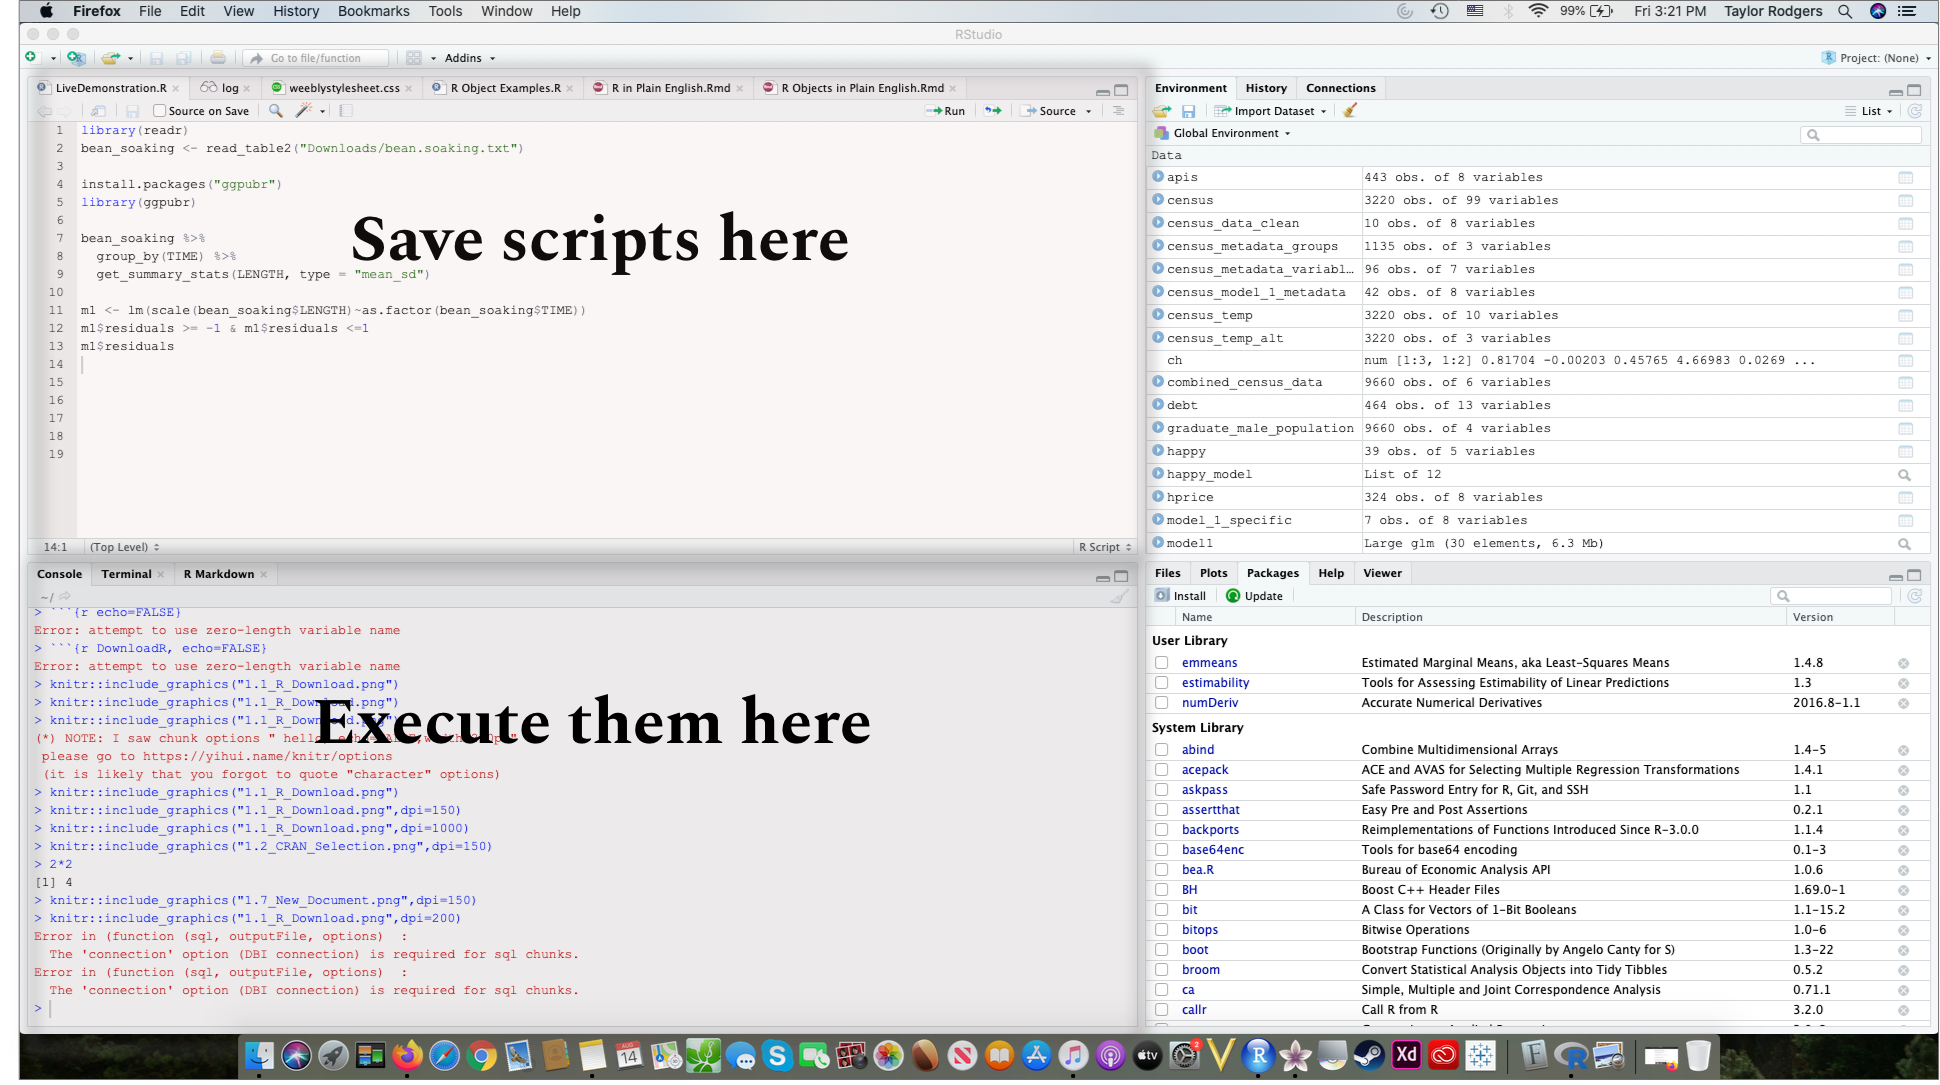
\includegraphics[width=0.75\linewidth]{1.18_Console_Source_Comparison} \end{center}

This pane also has a \textbf{Terminal} and an \textbf{R Markdown} tab (if you have the latter installed). The \textbf{Terminal} allows you to enter commands to interact with your computer. IT professionals use this frequently. You probably won't.

\textbf{R Markdown} may not appear for you yet. I'll explain what R Markdown in a later chapter, but this tab merely shows the log for producing an R Markdown export.

The top right pane includes \textbf{environment}, \textbf{history}, and \textbf{connections} as tabular options.

\begin{center}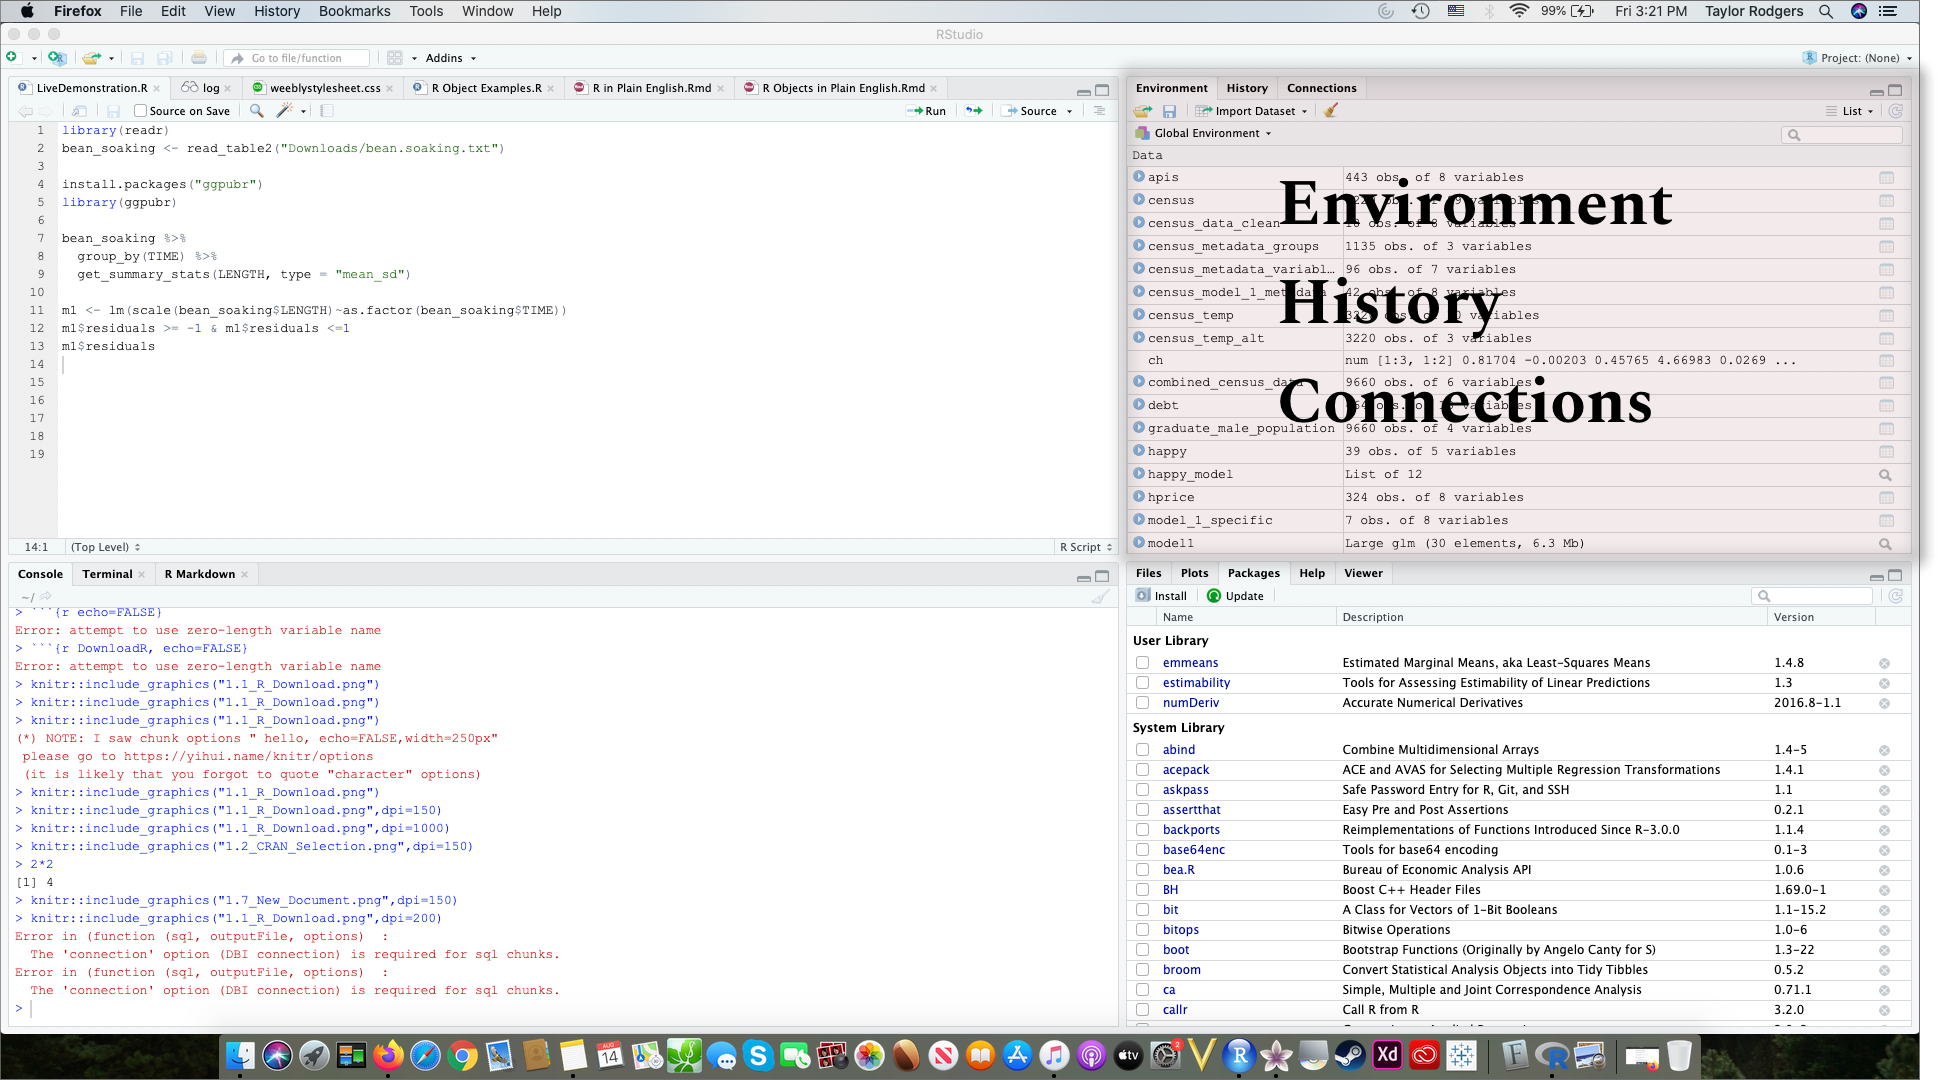
\includegraphics[width=0.75\linewidth]{1.19_RStudio_EnvironmentOthers} \end{center}

\textbf{Environment} is very handy and it's something that sets RStudio apart from the base version. It shows \textbf{objects} with assigned names that are saved in your environment.

\begin{center}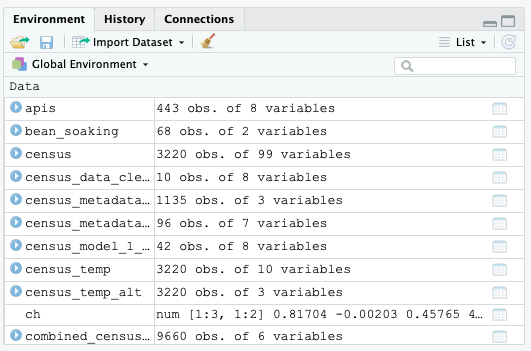
\includegraphics[width=0.75\linewidth]{1.20_Environment_Tab} \end{center}

We'll go into objects extensively in the next chapter. Along with packages, \emph{they're the most important component of R programming.} What you need to remember here is that the environment tab in this top right pane tells you what you have saved.

The \textbf{history} section is one I don't use too often, but I could see why some people would find it handy. It tells you what commands you've run during your R session. So anything you input in your console will show up here as a record.

\begin{center}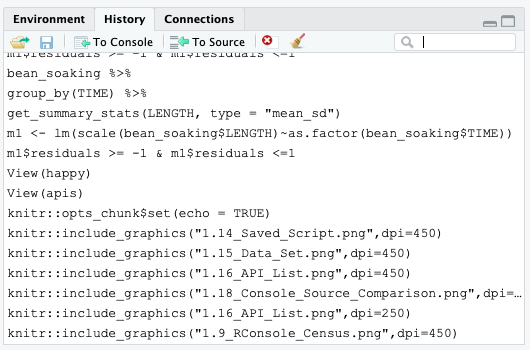
\includegraphics[width=0.75\linewidth]{1.21_History_Tab} \end{center}

The \textbf{connection} tab is useful for those who want to connect to a database or data warehouse.

\begin{center}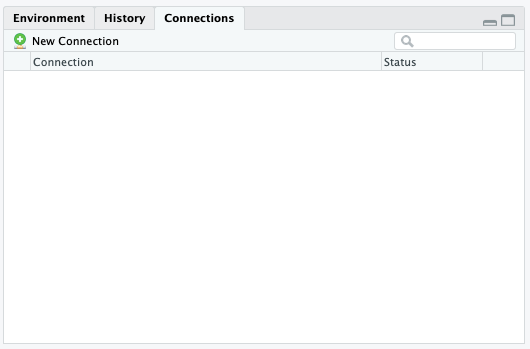
\includegraphics[width=0.75\linewidth]{1.22_Connections_Tab} \end{center}

If you're a researcher, you may not use this much. If you work with databases in any capacity, this will make it easier to simply query data directly from the database, as opposed to importing it in via CSV files or spreadsheets.

The bottom right pane is a very useful addition provided by RStudio. It contains a separate tab for \textbf{files}, \textbf{plots}, \textbf{packages}, \textbf{help}, and \textbf{viewer}.

\begin{center}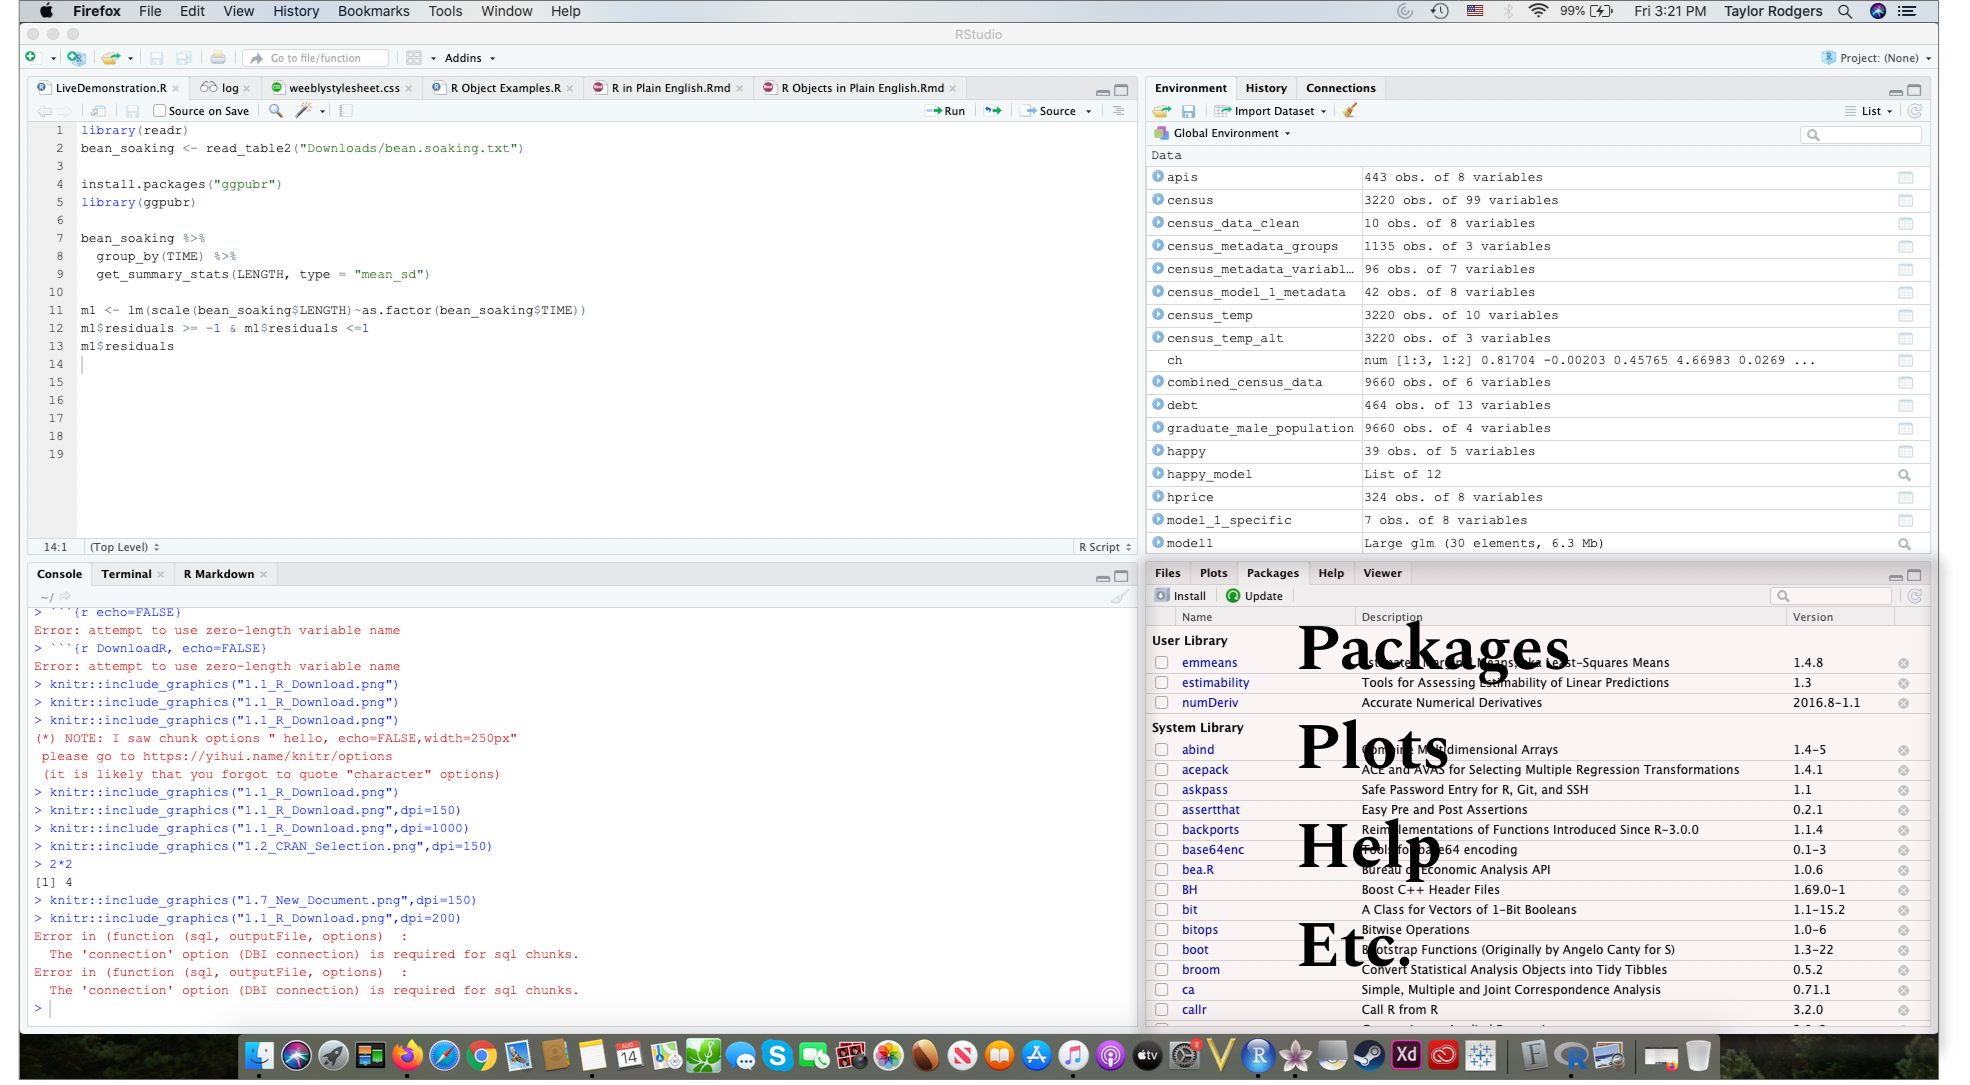
\includegraphics[width=0.75\linewidth]{1.23_RStudio_PackagesEtc} \end{center}

I'm going to start with the \textbf{packages} tab. If you recall, I said that packages are what makes R such a useful programming language. It allows you to customize and import functions to suit your needs.

\begin{center}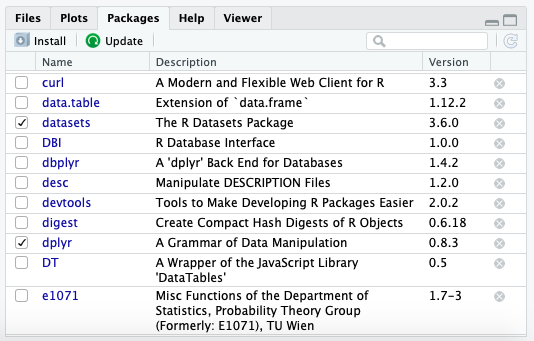
\includegraphics[width=0.75\linewidth]{1.24_Packages} \end{center}

This is a useful little tab. If you open a previously saved script, you may find out that some functions need a package to execute. This tab can tell you whether you need to install that package or simply need to re-load it.

I'll have a whole chapter dedicated to finding packages, installing packages, and loading packages.

\textbf{Plots} is a tab that displays any plots you create using graphical commands. We'll cover this in more detail in a later chapter.

\begin{center}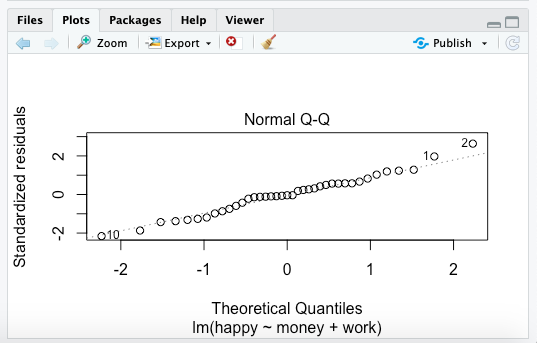
\includegraphics[width=0.75\linewidth]{1.25_Plots} \end{center}

\textbf{Help} is a super helpful tab. You can find the extensive R documentation there that explains many of the functionality of R and how it operates. It also will display information you look up on packages and functions you download.

\begin{center}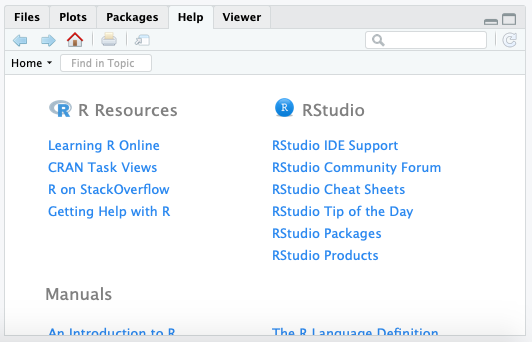
\includegraphics[width=0.75\linewidth]{1.26_Help} \end{center}

If you ever add a \texttt{?} before a function, it will display the documentation in the help section.

Try adding the following command to the R console and see what happens:

\begin{Shaded}
\begin{Highlighting}[]
\NormalTok{  ?lm}
\end{Highlighting}
\end{Shaded}

Here's what it should look like on your screen:

\begin{center}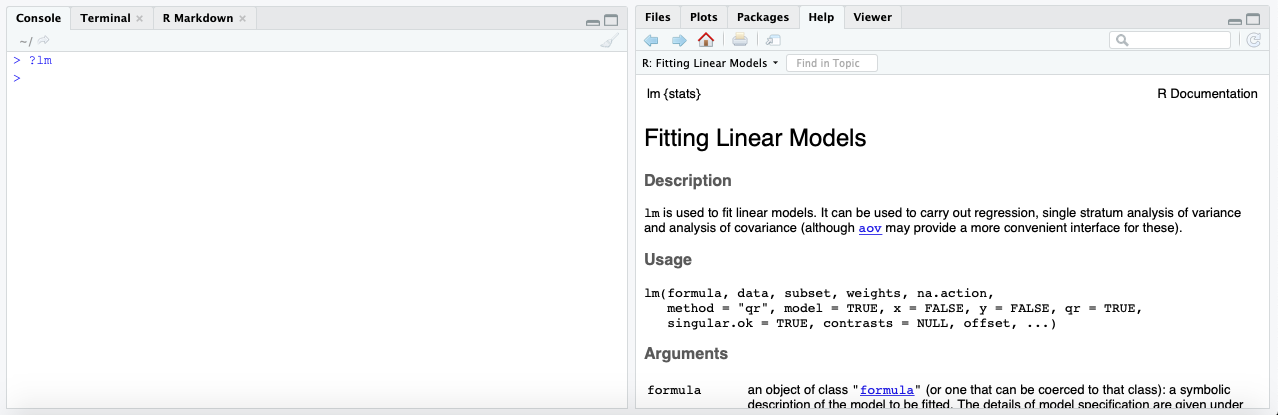
\includegraphics[width=0.75\linewidth]{1.27_HelpLookup} \end{center}

Don't forget about this trick! It helps a lot!

Lastly, we have the \textbf{files} and the \textbf{viewer} tab.

\begin{center}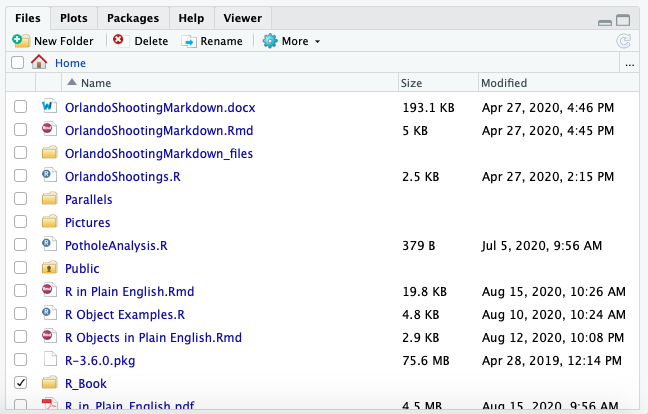
\includegraphics[width=0.75\linewidth]{1.28_Files} \end{center}

The \textbf{files} tab displays all the files you can open in RStudio for a given folder. This is helpful because you don't have to specify a file path when loading files listed here.

The \textbf{viewer} tab allows to display non-R related outputs, such as a website or JavaScript graphics.

\hypertarget{things-to-remember-1}{%
\section{Things to Remember}\label{things-to-remember-1}}

\begin{itemize}
\tightlist
\item
  R packages contains new functions that allow you to use R for your own specific purposes
\item
  RStudio is a more user friendly interface
\end{itemize}

\hypertarget{objects}{%
\chapter{R Objects Types}\label{objects}}

R uses \textbf{objects} to store and interact with data and there are various object types. That probably means little to you now, but understanding these differences will make R programming easier -- whatever your R programming goals.

In fact, I say it's better to understand how these objects interact with one another over memorizing every base function and package out there.

That's different from the approach I took to learning R. When I learned R, I went straight to learning the base functions. You know, the cool stuff that does the regression analysis and confidence intervals and whatnot.

That didn't work out well for me. I was coming from a SQL background and thought data worked in a similar way with R.

Had I started by learning the objects first, I would've saved a lot more time. I would've done less data manipulation in SQL or Excel and made simpler, more scalable R code.

\hypertarget{why-do-objects-matter}{%
\section{Why Do Objects Matter?}\label{why-do-objects-matter}}

Almost everything you program in R does one of the following:

\begin{itemize}
\tightlist
\item
  Reads an object
\item
  Modifies an object
\item
  Produces an object
\item
  Calls upon a pre-existing object
\end{itemize}

The simple code below utilizes five different object types:

\begin{Shaded}
\begin{Highlighting}[]
\KeywordTok{confint.lm}\NormalTok{(happy_model)}
\end{Highlighting}
\end{Shaded}

This code for calculating confidence intervals calls upon a base \textbf{function}, evaluates an existing \textbf{list}, creates several \textbf{vectors} and an \textbf{array} to perform the analysis, and then outputs a \textbf{matrix}. All five are objects. (You can see the function's script by pasting \texttt{stats::confint.lm} in your console.)

Understanding this will help you understand how R can seem to ``guess'' what it's supposed to do based on the data inputs.

\hypertarget{understanding-object-types-makes-it-easier-to-transform-and-analyze}{%
\section{Understanding Object Types Makes It Easier to Transform and Analyze}\label{understanding-object-types-makes-it-easier-to-transform-and-analyze}}

Pulling data from one object type is different than pulling data from another. This makes it confusing for people who learned about data through SQL, as opposed to other programming languages.

For example, the following code will select most data types in SQL:

\begin{Shaded}
\begin{Highlighting}[]
\KeywordTok{SELECT}
\NormalTok{  Field1,}
\NormalTok{  Field2,}
\NormalTok{  Field3,}
\NormalTok{  Field4}
\KeywordTok{FROM}
\NormalTok{  Data_Set}
\end{Highlighting}
\end{Shaded}

That's different from R. Data selection in R depends on the object type.

For example, using the command \texttt{{[}6{]}} next to the object name will select a single value from a \textbf{vector} object\ldots{}

\begin{Shaded}
\begin{Highlighting}[]
\NormalTok{money[}\DecValTok{6}\NormalTok{]}
\end{Highlighting}
\end{Shaded}

\begin{verbatim}
## [1] 175
\end{verbatim}

But that won't work for a \textbf{list} object below\ldots{}

\begin{Shaded}
\begin{Highlighting}[]
\NormalTok{happy_model[}\DecValTok{6}\NormalTok{]}
\end{Highlighting}
\end{Shaded}

\begin{verbatim}
## $assign
## [1] 0 1 2
\end{verbatim}

To learn how to select, transform, and analyze data in R requires that you learn the underlying structure first. Once you do that, everything else makes more sense.

\hypertarget{the-basic-objects-to-remember}{%
\section{The Basic Objects to Remember}\label{the-basic-objects-to-remember}}

Down below are the common objects in R:

\begin{enumerate}
\def\labelenumi{\arabic{enumi}.}
\tightlist
\item
  Vectors
\item
  Matrices / Arrays
\item
  Data Frames
\item
  Lists
\item
  Factors
\item
  Functions
\end{enumerate}

We won't talk about functions in this chapter since they need their own chapter to explain how they work.

\hypertarget{vectors}{%
\section{Vectors}\label{vectors}}

Vector is the most basic object within R and there are seven ``modes'' of vectors: logical, numeric, integer, complex, character, date, and raw.

If that seems to be a lot to remember, don't worry. I'd focus on remembering \textbf{logical}, \textbf{numeric}, and \textbf{character} right now. Those are the ones you'll use most often. Others we'll cover as needed.

Vectors can only be one mode at a time. What that means in plain English is that R can't have a word and a number in the same vector.

You can use the code below to create and view a \textbf{logical} vector:

\begin{Shaded}
\begin{Highlighting}[]
\NormalTok{v1 <-}\StringTok{ }\KeywordTok{c}\NormalTok{(}\OtherTok{TRUE}\NormalTok{,}\OtherTok{FALSE}\NormalTok{,}\OtherTok{TRUE}\NormalTok{)}
\NormalTok{v1}
\end{Highlighting}
\end{Shaded}

\begin{verbatim}
## [1]  TRUE FALSE  TRUE
\end{verbatim}

What this code does is create a vector using the \texttt{c(input,\ input)} notation. It then assigns the vector the name \textbf{v1} using the \texttt{\textless{}–} notation. (A shortcut to the \texttt{\textless{}-} command is \textbf{Option+``-''}.)

You build a \textbf{character} vector in the same way, only that you use \texttt{c("input",\ "input")} notation instead:

\begin{Shaded}
\begin{Highlighting}[]
\NormalTok{v2 <-}\StringTok{ }\KeywordTok{c}\NormalTok{(}\StringTok{"Hola"}\NormalTok{,}\StringTok{"Howdy"}\NormalTok{,}\StringTok{"Hello"}\NormalTok{)}
\NormalTok{v2}
\end{Highlighting}
\end{Shaded}

\begin{verbatim}
## [1] "Hola"  "Howdy" "Hello"
\end{verbatim}

And a \textbf{numeric} vector (like the name suggests) looks like this:

\begin{Shaded}
\begin{Highlighting}[]
\NormalTok{v3 <-}\StringTok{ }\KeywordTok{c}\NormalTok{(}\DecValTok{1}\OperatorTok{:}\DecValTok{3}\NormalTok{)}
\NormalTok{v3}
\end{Highlighting}
\end{Shaded}

\begin{verbatim}
## [1] 1 2 3
\end{verbatim}

The code above used the \texttt{c(n1:n2)} notation to create a range of values from n1 to n2, where n1 is 1 and n2 is 4. You can also use notations such as \texttt{c(n1,\ n2,\ n3,\ n4)} or like \texttt{c(n1:n4,\ n5:n6)}.

Play around with the code below and see what kind numeric vectors you can make!

\begin{Shaded}
\begin{Highlighting}[]
\NormalTok{v4 <-}\StringTok{ }\KeywordTok{c}\NormalTok{(}\DecValTok{4}\OperatorTok{:}\DecValTok{6}\NormalTok{,}\DecValTok{1}\OperatorTok{:}\DecValTok{7}\NormalTok{)}
\NormalTok{v4}
\end{Highlighting}
\end{Shaded}

\begin{verbatim}
##  [1] 4 5 6 1 2 3 4 5 6 7
\end{verbatim}

\begin{Shaded}
\begin{Highlighting}[]
\NormalTok{v5 <-}\StringTok{ }\KeywordTok{c}\NormalTok{(}\DecValTok{1}\NormalTok{,}\DecValTok{5}\NormalTok{,}\DecValTok{5}\NormalTok{,}\DecValTok{2}\NormalTok{,}\DecValTok{1}\NormalTok{,}\DecValTok{4}\NormalTok{)}
\NormalTok{v5}
\end{Highlighting}
\end{Shaded}

\begin{verbatim}
## [1] 1 5 5 2 1 4
\end{verbatim}

I said before that vectors can only be one ``mode'' or data type at a time. What that means is that if you attempt to mix numbers or a logical value with a character, it simply changes all values to a character.

The code down below takes our previously made vectors, one a numeric and the other a character, and combines them into a single vector. As you can see by the quotation " " marks around the output, it's changed all the numeric values into characters.

\begin{Shaded}
\begin{Highlighting}[]
\NormalTok{v6 <-}\StringTok{ }\KeywordTok{c}\NormalTok{(v2,v3)}
\NormalTok{v6}
\end{Highlighting}
\end{Shaded}

\begin{verbatim}
## [1] "Hola"  "Howdy" "Hello" "1"     "2"     "3"
\end{verbatim}

The vector seems basic and not at all like the data sets you'll be using. That might make you ask -- will I even use vectors?

Yes. Yes, you will.

The more complex object, data frame, is comprised of individual vectors. (We'll cover more about the data frame object later).

Many functions will also \textbf{output} data in vector form or produce a list composed of vectors.

Vectors are also useful as \textbf{inputs} into other functions, as well. If you look below, I used a function from the \texttt{censusapi} package. I create a vector beforehand and then use it as an input for the function below it.

\begin{Shaded}
\begin{Highlighting}[]
\NormalTok{variable_list <-}\StringTok{ }
\StringTok{    }\KeywordTok{c}\NormalTok{(}\StringTok{"B15001_003E"}\NormalTok{,}\StringTok{"B15001_004E"}\NormalTok{,}\StringTok{"B15001_005E"}\NormalTok{,}
      \StringTok{"B15001_044E"}\NormalTok{,}\StringTok{"B15001_045E"}\NormalTok{,}\StringTok{"B15001_046E"}\NormalTok{)}
\KeywordTok{getCensus}\NormalTok{(}\DataTypeTok{name=}\StringTok{"acs/acs5"}\NormalTok{,}
          \DataTypeTok{vintage=}\StringTok{"2018"}\NormalTok{,}
          \DataTypeTok{vars=}\KeywordTok{c}\NormalTok{(}\StringTok{"NAME"}\NormalTok{,variable_list),}
          \DataTypeTok{region=}\StringTok{"state:*"}\NormalTok{)}
\end{Highlighting}
\end{Shaded}

You can use vectors in this way on a larger scale. For example, if you write a long script with many functions and references, vectors allow you to create a set of parameters at the beginning.

\hypertarget{matrices-and-arrays}{%
\section{Matrices and Arrays}\label{matrices-and-arrays}}

Matrices and arrays in R are multi-dimensional vectors. Matrices have multiple rows and columns. Arrays have two or more dimensions. (More on that distinction in a bit).

Like their vector counterpart, all matrix / array values must be the same mode or data type -- not a mix. That means if you can't have a numeric value alongside a character value.

Here's an example of a matrix:

\begin{Shaded}
\begin{Highlighting}[]
\NormalTok{matrix1 <-}\StringTok{ }\KeywordTok{matrix}\NormalTok{(}\KeywordTok{c}\NormalTok{(}\DecValTok{2}\NormalTok{,}\DecValTok{0}\NormalTok{,}\DecValTok{1}\NormalTok{,}\DecValTok{3}\NormalTok{),}\DataTypeTok{nrow=}\DecValTok{2}\NormalTok{,}\DataTypeTok{ncol=}\DecValTok{2}\NormalTok{)}
\NormalTok{matrix1}
\end{Highlighting}
\end{Shaded}

\begin{verbatim}
##      [,1] [,2]
## [1,]    2    1
## [2,]    0    3
\end{verbatim}

Why would R programmers want this? It comes back to the R's use as a statistical programming language. For example, multiple linear regression often has combined variables, which involves multiplying two matrices together.

Providing these two object types in R that are solely for numeric values makes this easier.

For example, you can multiply these two matrices together with the \texttt{\%*\%} command and get the same results you would by using matrix algebra:

\begin{Shaded}
\begin{Highlighting}[]
\NormalTok{matrix1 <-}\StringTok{ }\KeywordTok{matrix}\NormalTok{(}\KeywordTok{c}\NormalTok{(}\DecValTok{2}\NormalTok{,}\DecValTok{0}\NormalTok{,}\DecValTok{1}\NormalTok{,}\DecValTok{3}\NormalTok{),}\DataTypeTok{nrow=}\DecValTok{2}\NormalTok{,}\DataTypeTok{ncol=}\DecValTok{2}\NormalTok{)}
\NormalTok{matrix1}
\end{Highlighting}
\end{Shaded}

\begin{verbatim}
##      [,1] [,2]
## [1,]    2    1
## [2,]    0    3
\end{verbatim}

\begin{Shaded}
\begin{Highlighting}[]
\NormalTok{matrix2 <-}\StringTok{ }\KeywordTok{matrix}\NormalTok{(}\KeywordTok{c}\NormalTok{(}\DecValTok{5}\NormalTok{,}\DecValTok{7}\NormalTok{),}\DataTypeTok{nrow=}\DecValTok{2}\NormalTok{)}
\NormalTok{matrix2}
\end{Highlighting}
\end{Shaded}

\begin{verbatim}
##      [,1]
## [1,]    5
## [2,]    7
\end{verbatim}

\begin{Shaded}
\begin{Highlighting}[]
\NormalTok{matrix1 }\OperatorTok\StringTok{ }\NormalTok{matrix2 }\CommentTok{#multiplication}
\end{Highlighting}
\end{Shaded}

\begin{verbatim}
##      [,1]
## [1,]   17
## [2,]   21
\end{verbatim}

That's the same as if you did it yourself by hand.
\[
 \begin{bmatrix}
  2 & 1\\
  0 & 3 \\
 \end{bmatrix}
 \begin{bmatrix}
  5\\
  7\\
 \end{bmatrix}
 =
 \begin{bmatrix}
  17\\
  21\\
 \end{bmatrix} \]

Unless you're building the functions that calculate this, I doubt you'll use matrices or arrays all that much. However, it's handy to know what they are and how they can be used. They're often the output of functions as well.

Arrays are more complex than their simple 2-D counterpart. Instead of a single set of rows and columns, you'll have multiple dimensions added on top.

\begin{Shaded}
\begin{Highlighting}[]
\NormalTok{matrix3 <-}\StringTok{ }\KeywordTok{matrix}\NormalTok{(}\KeywordTok{c}\NormalTok{(}\DecValTok{2}\NormalTok{,}\DecValTok{0}\NormalTok{,}\DecValTok{1}\NormalTok{,}\DecValTok{4}\NormalTok{,}\DecValTok{5}\NormalTok{,}\DecValTok{2}\NormalTok{,}\DecValTok{3}\NormalTok{,}\DecValTok{4}\NormalTok{),}\DataTypeTok{nrow=}\DecValTok{4}\NormalTok{,}\DataTypeTok{ncol=}\DecValTok{2}\NormalTok{)}
\NormalTok{matrix4 <-}\StringTok{ }\KeywordTok{matrix}\NormalTok{(}\KeywordTok{c}\NormalTok{(}\DecValTok{4}\NormalTok{,}\DecValTok{3}\NormalTok{,}\DecValTok{5}\NormalTok{,}\DecValTok{2}\NormalTok{,}\DecValTok{1}\NormalTok{,}\DecValTok{6}\NormalTok{,}\DecValTok{4}\NormalTok{,}\DecValTok{5}\NormalTok{),}\DataTypeTok{nrow=}\DecValTok{4}\NormalTok{,}\DataTypeTok{ncol=}\DecValTok{2}\NormalTok{)}
\NormalTok{matrix5 <-}\StringTok{ }\KeywordTok{matrix}\NormalTok{(}\KeywordTok{c}\NormalTok{(}\DecValTok{1}\NormalTok{,}\DecValTok{3}\NormalTok{,}\DecValTok{1}\NormalTok{,}\DecValTok{2}\NormalTok{,}\DecValTok{3}\NormalTok{,}\DecValTok{5}\NormalTok{,}\DecValTok{6}\NormalTok{,}\DecValTok{2}\NormalTok{),}\DataTypeTok{nrow=}\DecValTok{4}\NormalTok{,}\DataTypeTok{ncol=}\DecValTok{2}\NormalTok{)}
\NormalTok{array1 <-}\StringTok{ }\KeywordTok{array}\NormalTok{(}\KeywordTok{c}\NormalTok{(matrix3,matrix4,matrix5),}
                \DataTypeTok{dim=}\KeywordTok{c}\NormalTok{(}\DecValTok{4}\NormalTok{,}\DecValTok{2}\NormalTok{,}\DecValTok{3}\NormalTok{))}
\NormalTok{array1}
\end{Highlighting}
\end{Shaded}

\begin{verbatim}
## , , 1
## 
##      [,1] [,2]
## [1,]    2    5
## [2,]    0    2
## [3,]    1    3
## [4,]    4    4
## 
## , , 2
## 
##      [,1] [,2]
## [1,]    4    1
## [2,]    3    6
## [3,]    5    4
## [4,]    2    5
## 
## , , 3
## 
##      [,1] [,2]
## [1,]    1    3
## [2,]    3    5
## [3,]    1    6
## [4,]    2    2
\end{verbatim}

If the output up above looks like gibberish, don't worry -- most people think it's confusing when they first see it. That's because the R user interface doesn't make it visually intuitive as to how the array operates.

Let's use a picture to visualize this instead. Think of it as if each matrix as a separate entity within the array:

\begin{center}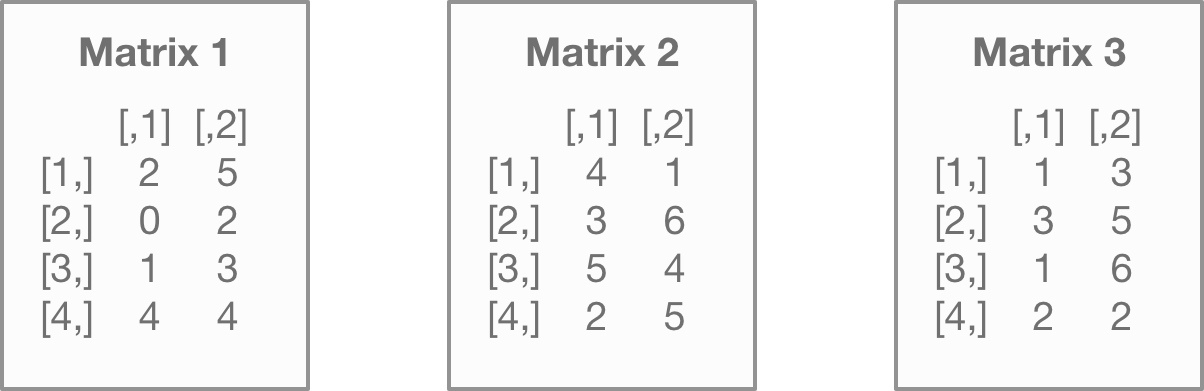
\includegraphics[width=0.5\linewidth]{1.29_Arrays_Flat} \end{center}

What the array does is simply \emph{stack} them on top of each other:

\begin{center}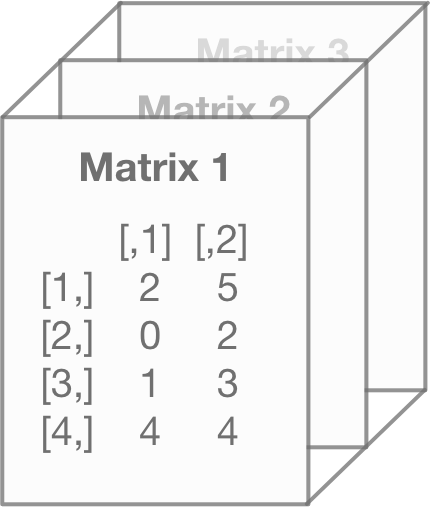
\includegraphics[width=0.15\linewidth]{1.30_Arrays_Stacked} \end{center}

Since arrays with three dimensions are merely stacked matrices, that means each matrix within the array must have the same number of columns and rows.

\hypertarget{data-frames}{%
\section{Data Frames}\label{data-frames}}

Data frame is the object type that's most similar to what you'd find in a SQL database. What I mean by that is that it's organized and referenced by columns and can have many, many rows.

And most importantly, it can contain both numeric and character values! (Earth shattering, I know!)

I like to think of a data frame as a way to combine vectors. As a matter of fact, you can build a data frame doing just that.

Take this code below and run it. You'll see that we make individual vectors containing data on James Bond movies\footnote{\citet{noauthor_james_nodate}} and we then combine it into a data frame.

\begin{Shaded}
\begin{Highlighting}[]
\NormalTok{filmname <-}\StringTok{ }
\StringTok{      }\KeywordTok{c}\NormalTok{(}\StringTok{"Skyfall"}\NormalTok{,}\StringTok{"Thunderball"}\NormalTok{,}\StringTok{"Goldfinger"}\NormalTok{,}
        \StringTok{"Spectre"}\NormalTok{,}\StringTok{"Live and Let Die"}\NormalTok{,}
        \StringTok{"You Only Live Twice"}\NormalTok{,}
        \StringTok{"The Spy Who Loved Me"}\NormalTok{,}\StringTok{"Casino Royale"}\NormalTok{,}
        \StringTok{"Moonraker"}\NormalTok{,}\StringTok{"Diamonds Are Forever"}\NormalTok{,}
        \StringTok{"Quantum of Solace"}\NormalTok{,}\StringTok{"From Russia with Love"}\NormalTok{,}
        \StringTok{"Die Another Day"}\NormalTok{,}\StringTok{"Goldeneye"}\NormalTok{,}
        \StringTok{"On Her Majesty's Secret Service"}\NormalTok{,}
        \StringTok{"The World is Not Enough"}\NormalTok{,}
        \StringTok{"For Your Eyes Only"}\NormalTok{,}\StringTok{"Tomorrow Never Dies"}\NormalTok{,}
        \StringTok{"The Man with the Golden Gun"}\NormalTok{,}
        \StringTok{"Dr. No"}\NormalTok{,}\StringTok{"Octopussy"}\NormalTok{,}
        \StringTok{"The Living Daylights"}\NormalTok{,}\StringTok{"A View to a Kill"}\NormalTok{,}
        \StringTok{"Licence to Kill"}\NormalTok{)}
\NormalTok{year <-}\StringTok{ }\KeywordTok{c}\NormalTok{(}\StringTok{"2012"}\NormalTok{,}\StringTok{"1965"}\NormalTok{,}\StringTok{"1964"}\NormalTok{,}\StringTok{"2015"}\NormalTok{,}
          \StringTok{"1973"}\NormalTok{,}\StringTok{"1967"}\NormalTok{,}\StringTok{"1977"}\NormalTok{,}\StringTok{"2006"}\NormalTok{,}
          \StringTok{"1979"}\NormalTok{,}\StringTok{"1971"}\NormalTok{,}\StringTok{"2008"}\NormalTok{,}\StringTok{"1963"}\NormalTok{,}
          \StringTok{"2002"}\NormalTok{,}\StringTok{"1995"}\NormalTok{,}\StringTok{"1969"}\NormalTok{,}\StringTok{"1999"}\NormalTok{,}
          \StringTok{"1981"}\NormalTok{,}\StringTok{"1997"}\NormalTok{,}\StringTok{"1974"}\NormalTok{,}\StringTok{"1962"}\NormalTok{,}
          \StringTok{"1983"}\NormalTok{,}\StringTok{"1987"}\NormalTok{,}\StringTok{"1985"}\NormalTok{,}\StringTok{"1989"}\NormalTok{)}
\NormalTok{actor <-}\StringTok{ }\KeywordTok{c}\NormalTok{(}\StringTok{"Daniel Craig"}\NormalTok{,}\StringTok{"Sean Connery"}\NormalTok{,}
           \StringTok{"Sean Connery"}\NormalTok{,}\StringTok{"Daniel Craig"}\NormalTok{,}
           \StringTok{"Roger Moore"}\NormalTok{,}\StringTok{"Sean Connery"}\NormalTok{,}
           \StringTok{"Roger Moore"}\NormalTok{,}\StringTok{"Daniel Craig"}\NormalTok{,}
           \StringTok{"Roger Moore"}\NormalTok{,}\StringTok{"Sean Connery"}\NormalTok{,}
           \StringTok{"Daniel Craig"}\NormalTok{,}\StringTok{"Sean Connery"}\NormalTok{,}
           \StringTok{"Pierce Brosnan"}\NormalTok{,}\StringTok{"Pierce Brosnan"}\NormalTok{,}
           \StringTok{"George Lazenby"}\NormalTok{,}\StringTok{"Pierce Brosnan"}\NormalTok{,}
           \StringTok{"Roger Moore"}\NormalTok{,}\StringTok{"Pierce Brosnan"}\NormalTok{,}
           \StringTok{"Roger Moore"}\NormalTok{,}\StringTok{"Sean Connery"}\NormalTok{,}
           \StringTok{"Roger Moore"}\NormalTok{,}\StringTok{"Timothy Dalton"}\NormalTok{,}
           \StringTok{"Roger Moore"}\NormalTok{,}\StringTok{"Timothy Dalton"}\NormalTok{)}
\NormalTok{gross <-}\StringTok{ }\KeywordTok{c}\NormalTok{(}\DecValTok{1108561008}\NormalTok{,}\DecValTok{1014941117}\NormalTok{,}\DecValTok{912257512}\NormalTok{,}
           \DecValTok{880669186}\NormalTok{,}\DecValTok{825110761}\NormalTok{,}\DecValTok{756544419}\NormalTok{,}
           \DecValTok{692713752}\NormalTok{,}\DecValTok{669789482}\NormalTok{,}\DecValTok{655872400}\NormalTok{,}
           \DecValTok{648514469}\NormalTok{,}\DecValTok{622246378}\NormalTok{,}\DecValTok{576277964}\NormalTok{,}
           \DecValTok{543639638}\NormalTok{,}\DecValTok{529548711}\NormalTok{,}\DecValTok{505899782}\NormalTok{,}
           \DecValTok{491617153}\NormalTok{,}\DecValTok{486468881}\NormalTok{,}\DecValTok{478946402}\NormalTok{,}
           \DecValTok{448249281}\NormalTok{,}\DecValTok{440759072}\NormalTok{,}\DecValTok{426244352}\NormalTok{,}
           \DecValTok{381088866}\NormalTok{,}\DecValTok{321172633}\NormalTok{,}\DecValTok{285157191}\NormalTok{)}\OperatorTok{/}\DecValTok{1000000}
\NormalTok{bond <-}\StringTok{ }\KeywordTok{data.frame}\NormalTok{(}\DataTypeTok{filmname=}\NormalTok{filmname,}
                   \DataTypeTok{year=}\NormalTok{year,}
                   \DataTypeTok{actor=}\NormalTok{actor,}
                   \DataTypeTok{gross=}\NormalTok{gross)}
\end{Highlighting}
\end{Shaded}

And if you use the \texttt{\$} sign, as we discussed before, you can re-select the individual vectors back out of it.

\begin{Shaded}
\begin{Highlighting}[]
\NormalTok{bond}\OperatorTok{$}\NormalTok{filmname}
\end{Highlighting}
\end{Shaded}

\begin{verbatim}
##  [1] "Skyfall"                         "Thunderball"                    
##  [3] "Goldfinger"                      "Spectre"                        
##  [5] "Live and Let Die"                "You Only Live Twice"            
##  [7] "The Spy Who Loved Me"            "Casino Royale"                  
##  [9] "Moonraker"                       "Diamonds Are Forever"           
## [11] "Quantum of Solace"               "From Russia with Love"          
## [13] "Die Another Day"                 "Goldeneye"                      
## [15] "On Her Majesty's Secret Service" "The World is Not Enough"        
## [17] "For Your Eyes Only"              "Tomorrow Never Dies"            
## [19] "The Man with the Golden Gun"     "Dr. No"                         
## [21] "Octopussy"                       "The Living Daylights"           
## [23] "A View to a Kill"                "Licence to Kill"
\end{verbatim}

If you want to select a single column and maintain the data frame object type, you have to use the following code:

\begin{Shaded}
\begin{Highlighting}[]
\NormalTok{bond[}\DecValTok{1}\NormalTok{]}
\end{Highlighting}
\end{Shaded}

\begin{verbatim}
##                           filmname
## 1                          Skyfall
## 2                      Thunderball
## 3                       Goldfinger
## 4                          Spectre
## 5                 Live and Let Die
## 6              You Only Live Twice
## 7             The Spy Who Loved Me
## 8                    Casino Royale
## 9                        Moonraker
## 10            Diamonds Are Forever
## 11               Quantum of Solace
## 12           From Russia with Love
## 13                 Die Another Day
## 14                       Goldeneye
## 15 On Her Majesty's Secret Service
## 16         The World is Not Enough
## 17              For Your Eyes Only
## 18             Tomorrow Never Dies
## 19     The Man with the Golden Gun
## 20                          Dr. No
## 21                       Octopussy
## 22            The Living Daylights
## 23                A View to a Kill
## 24                 Licence to Kill
\end{verbatim}

We'll go into further detail about selecting, transforming, and analyzing data frames later on. The way you go about it depends on whether you want to make efficient code or you want to make ``readable'' code for other analysts.

\hypertarget{factors}{%
\section{Factors}\label{factors}}

Factors take vectors (or data frame columns) and create categories to group the values. Confused? It's actually fairly simple.

Think back to the data frame we built for the Bond films. If you use the code below, you'll see the first six rows:

\begin{Shaded}
\begin{Highlighting}[]
\KeywordTok{head}\NormalTok{(bond)}
\end{Highlighting}
\end{Shaded}

\begin{verbatim}
##              filmname year        actor     gross
## 1             Skyfall 2012 Daniel Craig 1108.5610
## 2         Thunderball 1965 Sean Connery 1014.9411
## 3          Goldfinger 1964 Sean Connery  912.2575
## 4             Spectre 2015 Daniel Craig  880.6692
## 5    Live and Let Die 1973  Roger Moore  825.1108
## 6 You Only Live Twice 1967 Sean Connery  756.5444
\end{verbatim}

Now let's say you want a short list of the Bond actors. If you'll notice in the data set, the actor names like ``Daniel Craig'' and ``Sean Connery'' are used repeatedly. These are basically ways to group the data frame with a common field name - the actor who played Bond.

If we tried to get a list of these actors using the \texttt{levels()} function, it wouldn't work.

\begin{Shaded}
\begin{Highlighting}[]
\KeywordTok{levels}\NormalTok{(bond}\OperatorTok{$}\NormalTok{actor)}
\end{Highlighting}
\end{Shaded}

\begin{verbatim}
## NULL
\end{verbatim}

That's because it hasn't been \textbf{factored} yet.

This is a real simply fix. Simply use the \texttt{factor()} function and assign it to the field name within the data frame. You can use the code below to do this.

\begin{Shaded}
\begin{Highlighting}[]
\NormalTok{bond}\OperatorTok{$}\NormalTok{actor <-}\StringTok{ }\KeywordTok{factor}\NormalTok{(bond}\OperatorTok{$}\NormalTok{actor)}
\KeywordTok{levels}\NormalTok{(bond}\OperatorTok{$}\NormalTok{actor)}
\end{Highlighting}
\end{Shaded}

\begin{verbatim}
## [1] "Daniel Craig"   "George Lazenby" "Pierce Brosnan" "Roger Moore"   
## [5] "Sean Connery"   "Timothy Dalton"
\end{verbatim}

And this will also show up in the environment tab in the top left.

\begin{center}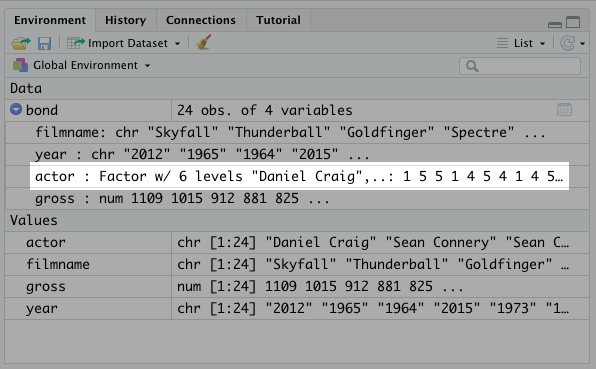
\includegraphics[width=0.5\linewidth]{1.31_Factors_in_Enviornment} \end{center}

R used to automatically factor character variables for you. However, that functionality was removed in a recent update.

You may see factors as a not-so-important object type, but that's not true. It comes in handy with regression analysis. Especially if your categorical variables are numeric.

For example, our Bond data frame may not include the actor name. It could simply have a number between 1 and 6 for the actor - with Sean Connery as 1 and Daniel Craig as 6. That means a regression analysis would've analyzed the actor as a continuous variable by default!

This also comes up with experiments that analyze the impact of medicine. It's not uncommon to label one drug as 1 and another drug as 2. That means you'd have to factor those drug codes so that your regression analysis reads them correctly.

\hypertarget{lists}{%
\section{Lists}\label{lists}}

Lists are objects that usually store other objects in a nice bundle. Those objects could be vectors, other lists, data frames, etc.

Many of the more complex R base functions produce lists. A common one is produced by the \texttt{lm()} function.

Use the code below to build a model with the James Bond data:

\begin{Shaded}
\begin{Highlighting}[]
\NormalTok{bondmodel <-}\StringTok{ }\KeywordTok{lm}\NormalTok{(gross}\OperatorTok{~}\NormalTok{actor,}\DataTypeTok{data=}\NormalTok{bond)}
\end{Highlighting}
\end{Shaded}

Now you can see the list this produces in the environment tab. As you can see, there's a lot in this list.

\begin{center}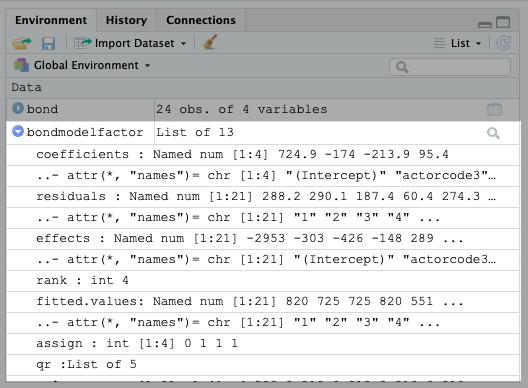
\includegraphics[width=0.5\linewidth]{1.34_List} \end{center}

You can also see what's in the list using the following code:

\begin{Shaded}
\begin{Highlighting}[]
\KeywordTok{names}\NormalTok{(bondmodel)}
\end{Highlighting}
\end{Shaded}

\begin{verbatim}
##  [1] "coefficients"  "residuals"     "effects"       "rank"         
##  [5] "fitted.values" "assign"        "qr"            "df.residual"  
##  [9] "contrasts"     "xlevels"       "call"          "terms"        
## [13] "model"
\end{verbatim}

This gets to the crux of why it's important to know when you're dealing with a list. It changes the way you select components of that list.

For example, let's say you want just the coefficients from a model you had built.

You can use the same \texttt{\$} symbol as before.

\begin{Shaded}
\begin{Highlighting}[]
\NormalTok{bondmodel}\OperatorTok{$}\NormalTok{coefficients}
\end{Highlighting}
\end{Shaded}

\begin{verbatim}
##         (Intercept) actorGeorge Lazenby actorPierce Brosnan    actorRoger Moore 
##           820.31651          -314.41673          -309.37854          -269.48336 
##   actorSean Connery actorTimothy Dalton 
##           -95.43409          -487.19349
\end{verbatim}

However, if you want to select a single coefficient, you have to use a number value afterwards:

\begin{Shaded}
\begin{Highlighting}[]
\NormalTok{bondmodel}\OperatorTok{$}\NormalTok{coefficients[}\DecValTok{4}\NormalTok{]}
\end{Highlighting}
\end{Shaded}

\begin{verbatim}
## actorRoger Moore 
##        -269.4834
\end{verbatim}

That's why it's important to know if you're pulling from a list or not. It changes the way that you select key parts of the data.

\hypertarget{functions}{%
\section{Functions}\label{functions}}

Functions are also an object. Most of the time, you'll be using a built-in function that is in the R base code or in a package you loaded.

However, you may find yourself building your own functions, which is handy if you don't want to search for a pre-existing one or need something unique to your situation.

We'll go into more detail about functions in a later chapter because of their complexity.

\hypertarget{things-to-remember-2}{%
\section{Things to Remember}\label{things-to-remember-2}}

\begin{itemize}
\tightlist
\item
  The key to understanding R is understanding objects
\item
  The object type changes the way you'll read, transform, and product data
\end{itemize}

\hypertarget{baserfilter}{%
\chapter{How to Filter and Transform Data in Base R}\label{baserfilter}}

In the last chapter, I explained the various object types in R. Now we want to learn how to \textbf{filter} and \textbf{transform} those objects. Notice how I didn't say filter and transform ``data''? That's because the methods you use to handle data in R heavily depend on the object type.

Before I explain those methods though, we need to cover operators.

\hypertarget{what-are-operators}{%
\section{What Are Operators?}\label{what-are-operators}}

If you're new to programming, then you're probably not familiar with the term \textbf{operator}. Operators, in plain English, modify or evaluate data. That's important to data transformation and filtering.

There are two types of operators in R: arithmetic and logical.

\textbf{Arithmetic} operators cover tasks like addition, subtraction, etc. You know? The basic math stuff. This is useful for data transformation and will be used in several examples later. Here are the common arithmetic operators:

\begin{tabular}{ll}
\toprule
label & symbol\\
\midrule
addition & +\\
subtraction & -\\
multiplication & *\\
division & /\\
exponent & \textasciicircum{}\\
\addlinespace
matrix multiplication & \%*\%\\
matrix division & \%/\%\\
\bottomrule
\end{tabular}

\textbf{Logical} operators takes the data and generates a TRUE or FALSE output, based on whether the data meets your requirement. This is more helpful for \emph{filtering} data than transforming. Here are the common logical operators:

\begin{tabular}{ll}
\toprule
label & symbol\\
\midrule
less than & <\\
greater than & >\\
less than or equal & <=\\
greater than or equal & >=\\
equal & ==\\
\addlinespace
does not equal & !=\\
and & \&\\
or & |\\
in & \%in\%\\
\bottomrule
\end{tabular}

Don't worry if you're unsure of how to use these just yet. You'll see examples for these in the next few sections. This is just for your easy reference.

\hypertarget{how-to-filter-and-transform-data-from-a-vector}{%
\section{How to Filter and Transform Data From a Vector}\label{how-to-filter-and-transform-data-from-a-vector}}

Vectors are the easiest object type to filter. Same with transforming the data within them.

If you want to reference or view the entire vector, you simply enter the name you assigned the object:

\begin{Shaded}
\begin{Highlighting}[]
\NormalTok{v5 <-}\StringTok{ }\KeywordTok{c}\NormalTok{(}\DecValTok{1}\NormalTok{,}\DecValTok{5}\NormalTok{,}\DecValTok{5}\NormalTok{,}\DecValTok{2}\NormalTok{,}\DecValTok{1}\NormalTok{,}\DecValTok{4}\NormalTok{)}
\NormalTok{v5}
\end{Highlighting}
\end{Shaded}

\begin{verbatim}
## [1] 1 5 5 2 1 4
\end{verbatim}

(Remember: the \texttt{\textless{}-} command allows you to name any object. You can use \textbf{Option+``-''} as a short-cut for \texttt{\textless{}-}.)

You also can select a single entry from a vector using the \texttt{{[}n{]}} notation:

\begin{Shaded}
\begin{Highlighting}[]
\NormalTok{v5 <-}\StringTok{ }\KeywordTok{c}\NormalTok{(}\DecValTok{1}\NormalTok{,}\DecValTok{5}\NormalTok{,}\DecValTok{5}\NormalTok{,}\DecValTok{2}\NormalTok{,}\DecValTok{1}\NormalTok{,}\DecValTok{4}\NormalTok{)}
\NormalTok{v5[}\DecValTok{3}\NormalTok{]}
\end{Highlighting}
\end{Shaded}

\begin{verbatim}
## [1] 5
\end{verbatim}

As you can see, the script above selected the third value from the vector.

You can select a range of entries by using the \texttt{{[}n:n{]}} notation.

\begin{Shaded}
\begin{Highlighting}[]
\NormalTok{v5 <-}\StringTok{ }\KeywordTok{c}\NormalTok{(}\DecValTok{1}\NormalTok{,}\DecValTok{5}\NormalTok{,}\DecValTok{5}\NormalTok{,}\DecValTok{2}\NormalTok{,}\DecValTok{1}\NormalTok{,}\DecValTok{4}\NormalTok{)}
\NormalTok{v5[}\DecValTok{3}\OperatorTok{:}\DecValTok{4}\NormalTok{]}
\end{Highlighting}
\end{Shaded}

\begin{verbatim}
## [1] 5 2
\end{verbatim}

And, as we've seen before, you can create a new vector by referencing old vectors!

\begin{Shaded}
\begin{Highlighting}[]
\NormalTok{v2 <-}\StringTok{ }\KeywordTok{c}\NormalTok{(}\StringTok{"Hola"}\NormalTok{,}\StringTok{"Howdy"}\NormalTok{,}\StringTok{"Hello"}\NormalTok{)}
\NormalTok{v7 <-}\StringTok{ }\KeywordTok{c}\NormalTok{(}\DecValTok{2}\OperatorTok{:}\DecValTok{4}\NormalTok{)}
\NormalTok{v8 <-}\StringTok{ }\KeywordTok{c}\NormalTok{(v2,v7)}
\NormalTok{v8}
\end{Highlighting}
\end{Shaded}

\begin{verbatim}
## [1] "Hola"  "Howdy" "Hello" "2"     "3"     "4"
\end{verbatim}

You can also use other base R functions to filter data.

For example, you may want to see the minimum or maximum value in a vector. You can use the \texttt{max()} and \texttt{min()} command to do so.

\begin{Shaded}
\begin{Highlighting}[]
\NormalTok{v5}
\end{Highlighting}
\end{Shaded}

\begin{verbatim}
## [1] 1 5 5 2 1 4
\end{verbatim}

\begin{Shaded}
\begin{Highlighting}[]
\KeywordTok{max}\NormalTok{(v5) }\CommentTok{# Max value}
\end{Highlighting}
\end{Shaded}

\begin{verbatim}
## [1] 5
\end{verbatim}

\begin{Shaded}
\begin{Highlighting}[]
\KeywordTok{min}\NormalTok{(v5) }\CommentTok{# Min value}
\end{Highlighting}
\end{Shaded}

\begin{verbatim}
## [1] 1
\end{verbatim}

And you can use logical operators as well. In the example below, I use the \texttt{\textgreater{}=} and \texttt{\&} operators to filter values:

\begin{Shaded}
\begin{Highlighting}[]
\NormalTok{v5 }\OperatorTok{>=}\StringTok{ }\DecValTok{2} \CommentTok{# Values greater than 2}
\end{Highlighting}
\end{Shaded}

\begin{verbatim}
## [1] FALSE  TRUE  TRUE  TRUE FALSE  TRUE
\end{verbatim}

\begin{Shaded}
\begin{Highlighting}[]
\NormalTok{v5 }\OperatorTok{>=}\StringTok{ }\DecValTok{3} \OperatorTok{&}\StringTok{ }\NormalTok{v5 }\OperatorTok{<=}\StringTok{ }\DecValTok{5} \CommentTok{# Values between 3 and 5}
\end{Highlighting}
\end{Shaded}

\begin{verbatim}
## [1] FALSE  TRUE  TRUE FALSE FALSE  TRUE
\end{verbatim}

We can also use the \texttt{\textbar{}} operator to find values that meet a criteria. For example, I filter the vector below to ``Hola'' and ``Howdy.''

\begin{Shaded}
\begin{Highlighting}[]
\NormalTok{v2}
\end{Highlighting}
\end{Shaded}

\begin{verbatim}
## [1] "Hola"  "Howdy" "Hello"
\end{verbatim}

\begin{Shaded}
\begin{Highlighting}[]
\NormalTok{v2 }\OperatorTok{==}\StringTok{ "Hola"} \OperatorTok{|}\StringTok{ }\NormalTok{v2 }\OperatorTok{==}\StringTok{ "Howdy"}
\end{Highlighting}
\end{Shaded}

\begin{verbatim}
## [1]  TRUE  TRUE FALSE
\end{verbatim}

You probably noticed that these logical operators only return a TRUE or FALSE statement. That makes sense since it is a \emph{logical} argument that's evaluated. However, we may want to see the actual values that meet the argument. This isn't important in an example like this, but it does come up later on for more complex objects.

To show the actual values where the logical argument is true, you use the \texttt{object\_name{[}argument{]}} notation. In the next few examples, I filter the vectors down to values that meet the arguments used in the last few examples:

\begin{Shaded}
\begin{Highlighting}[]
\NormalTok{v5[v5}\OperatorTok{>=}\DecValTok{2}\NormalTok{]}
\end{Highlighting}
\end{Shaded}

\begin{verbatim}
## [1] 5 5 2 4
\end{verbatim}

\begin{Shaded}
\begin{Highlighting}[]
\NormalTok{v5[v5 }\OperatorTok{>=}\StringTok{ }\DecValTok{3} \OperatorTok{&}\StringTok{ }\NormalTok{v5 }\OperatorTok{<=}\StringTok{ }\DecValTok{5}\NormalTok{]}
\end{Highlighting}
\end{Shaded}

\begin{verbatim}
## [1] 5 5 4
\end{verbatim}

\begin{Shaded}
\begin{Highlighting}[]
\NormalTok{v2[v2 }\OperatorTok{==}\StringTok{ "Hola"} \OperatorTok{|}\StringTok{ }\NormalTok{v2 }\OperatorTok{==}\StringTok{ "Howdy"}\NormalTok{]}
\end{Highlighting}
\end{Shaded}

\begin{verbatim}
## [1] "Hola"  "Howdy"
\end{verbatim}

In the examples above, I simply took the logical argument and plugged it into the brackets.

You can also change data easily when it comes to numeric vectors. For example, down below is a vector of box office revenue for James Bond films. Copy and paste this script into your R console and execute:

\begin{Shaded}
\begin{Highlighting}[]
\NormalTok{gross <-}\StringTok{ }
\StringTok{  }\KeywordTok{c}\NormalTok{(}\DecValTok{1108561008}\NormalTok{,}\DecValTok{1014941117}\NormalTok{,}\DecValTok{912257512}\NormalTok{,}\DecValTok{880669186}\NormalTok{,}
    \DecValTok{825110761}\NormalTok{,}\DecValTok{756544419}\NormalTok{,}\DecValTok{692713752}\NormalTok{,}\DecValTok{669789482}\NormalTok{,}
    \DecValTok{655872400}\NormalTok{,}\DecValTok{648514469}\NormalTok{,}\DecValTok{622246378}\NormalTok{,}\DecValTok{576277964}\NormalTok{,}
    \DecValTok{543639638}\NormalTok{,}\DecValTok{529548711}\NormalTok{,}\DecValTok{505899782}\NormalTok{,}\DecValTok{491617153}\NormalTok{,}
    \DecValTok{486468881}\NormalTok{,}\DecValTok{478946402}\NormalTok{,}\DecValTok{448249281}\NormalTok{,}\DecValTok{440759072}\NormalTok{,}
    \DecValTok{426244352}\NormalTok{,}\DecValTok{381088866}\NormalTok{,}\DecValTok{321172633}\NormalTok{,}\DecValTok{285157191}\NormalTok{)}
\NormalTok{gross}
\end{Highlighting}
\end{Shaded}

As you can see, the values are very large. To make our analysis easier, we can use an \emph{arithmetic} operator I showed earlier. In this scenario, I want to make the values smaller. So I'm going to divide it using the \texttt{/} operator.

\begin{Shaded}
\begin{Highlighting}[]
\NormalTok{gross}\OperatorTok{/}\DecValTok{1000000}
\end{Highlighting}
\end{Shaded}

You can also calculate individual values this way too.

\begin{Shaded}
\begin{Highlighting}[]
\NormalTok{gross[}\DecValTok{4}\NormalTok{]  }
\end{Highlighting}
\end{Shaded}

\begin{verbatim}
## [1] 880669186
\end{verbatim}

\begin{Shaded}
\begin{Highlighting}[]
\NormalTok{gross[}\DecValTok{4}\NormalTok{]}\OperatorTok{/}\DecValTok{100000}
\end{Highlighting}
\end{Shaded}

\begin{verbatim}
## [1] 8806.692
\end{verbatim}

And you can re-assign the value to a particular part of a vector using the methods we described above and the \texttt{\textless{}-} notation. For example, we can see below how we re-assign values based on the location.

\begin{Shaded}
\begin{Highlighting}[]
\NormalTok{v8 <-}\StringTok{ }\KeywordTok{c}\NormalTok{(}\DecValTok{1}\NormalTok{,}\DecValTok{5}\NormalTok{,}\DecValTok{5}\NormalTok{,}\DecValTok{2}\NormalTok{,}\DecValTok{1}\NormalTok{,}\DecValTok{4}\NormalTok{) }\CommentTok{# Creates the original vector}
\NormalTok{v8[}\DecValTok{6}\NormalTok{] <-}\StringTok{ }\DecValTok{8} \CommentTok{# Replaces the sixth value with an 8}
\NormalTok{v8[}\DecValTok{1}\OperatorTok{:}\DecValTok{3}\NormalTok{] <-}\StringTok{ }\KeywordTok{c}\NormalTok{(}\DecValTok{4}\NormalTok{,}\DecValTok{3}\NormalTok{,}\DecValTok{1}\NormalTok{) }\CommentTok{# Replaces the first three values}
\NormalTok{v8}
\end{Highlighting}
\end{Shaded}

\begin{verbatim}
## [1] 4 3 1 2 1 8
\end{verbatim}

\hypertarget{how-to-filter-and-transform-data-from-a-matrix}{%
\section{How to Filter and Transform Data From a Matrix}\label{how-to-filter-and-transform-data-from-a-matrix}}

Filtering the data within a matrix is both similar and different than a vector.

It's similar because we can use the \texttt{{[}n{]}} notation to select a single entry. We had done this before with a vector:

\begin{Shaded}
\begin{Highlighting}[]
\NormalTok{v5[}\DecValTok{2}\NormalTok{]}
\end{Highlighting}
\end{Shaded}

\begin{verbatim}
## [1] 5
\end{verbatim}

You can do the same for a matrix. If you run the code below, you'll re-create and view the matrix we used in the last chapter:

\begin{Shaded}
\begin{Highlighting}[]
\NormalTok{matrix1 <-}\StringTok{ }\KeywordTok{matrix}\NormalTok{(}\KeywordTok{c}\NormalTok{(}\DecValTok{2}\NormalTok{,}\DecValTok{0}\NormalTok{,}\DecValTok{1}\NormalTok{,}\DecValTok{3}\NormalTok{),}\DataTypeTok{nrow=}\DecValTok{2}\NormalTok{,}\DataTypeTok{ncol=}\DecValTok{2}\NormalTok{)}
\NormalTok{matrix1}
\end{Highlighting}
\end{Shaded}

\begin{verbatim}
##      [,1] [,2]
## [1,]    2    1
## [2,]    0    3
\end{verbatim}

And here you'll select the fourth value from that matrix using the \texttt{{[}4{]}} command:

\begin{Shaded}
\begin{Highlighting}[]
\NormalTok{matrix1[}\DecValTok{4}\NormalTok{]}
\end{Highlighting}
\end{Shaded}

\begin{verbatim}
## [1] 3
\end{verbatim}

Now that isn't very practical for a matrix. You may need to select a value from a specific row or column instead. This is where matrices are different from a vector. You'll want to use the \texttt{{[}r,c{]}} command to determine which values you want. In the example below, I select the second row and first column of the matrix.

\begin{Shaded}
\begin{Highlighting}[]
\NormalTok{matrix1[}\DecValTok{2}\NormalTok{,}\DecValTok{1}\NormalTok{]}
\end{Highlighting}
\end{Shaded}

\begin{verbatim}
## [1] 0
\end{verbatim}

We can make this easier on ourselves. Instead of specifying row or column numbers, we can give them names. That way, we can use the \texttt{{[}row\_name,column\_name{]}} notation to select data from a matrix. Down below, I give our previously created matrix row and column names.

\begin{Shaded}
\begin{Highlighting}[]
\KeywordTok{colnames}\NormalTok{(matrix1) <-}\StringTok{ }\KeywordTok{c}\NormalTok{(}\StringTok{"Col1"}\NormalTok{,}\StringTok{"Col2"}\NormalTok{)}
\KeywordTok{rownames}\NormalTok{(matrix1) <-}\StringTok{ }\KeywordTok{c}\NormalTok{(}\StringTok{"Row1"}\NormalTok{,}\StringTok{"Row2"}\NormalTok{)}
\NormalTok{matrix1[}\StringTok{"Row2"}\NormalTok{,}\StringTok{"Col1"}\NormalTok{]}
\end{Highlighting}
\end{Shaded}

\begin{verbatim}
## [1] 0
\end{verbatim}

We can also apply vector filtering methods to matrices. For example, I want to see what values are greater than 0.

\begin{Shaded}
\begin{Highlighting}[]
\NormalTok{matrix1 }\OperatorTok{>}\StringTok{ }\DecValTok{0} \CommentTok{# Returns true or false}
\end{Highlighting}
\end{Shaded}

\begin{verbatim}
##       Col1 Col2
## Row1  TRUE TRUE
## Row2 FALSE TRUE
\end{verbatim}

Funny enough though, you can't return the actual values that meet this criteria in a matrix form. It'll turn into a vector. That's because the output may not have the same number of columns and rows as the original matrix. So R assumes it'll need a one-dimensional object output.

\begin{Shaded}
\begin{Highlighting}[]
\NormalTok{matrix1[matrix1 }\OperatorTok{>}\StringTok{ }\DecValTok{0}\NormalTok{]}
\end{Highlighting}
\end{Shaded}

\begin{verbatim}
## [1] 2 1 3
\end{verbatim}

You can use the same techniques we outlined before with the vectors to transform the data within a matrix. Copy and paste the codes below to your R console and see the results. Feel free to play around with the inputs to see what happens.

\begin{Shaded}
\begin{Highlighting}[]
\NormalTok{matrix1 <-}\StringTok{ }\KeywordTok{matrix}\NormalTok{(}\KeywordTok{c}\NormalTok{(}\DecValTok{2}\NormalTok{,}\DecValTok{0}\NormalTok{,}\DecValTok{1}\NormalTok{,}\DecValTok{3}\NormalTok{),}\DataTypeTok{nrow=}\DecValTok{2}\NormalTok{,}\DataTypeTok{ncol=}\DecValTok{2}\NormalTok{)  }
\NormalTok{matrix1}
\end{Highlighting}
\end{Shaded}

\begin{verbatim}
##      [,1] [,2]
## [1,]    2    1
## [2,]    0    3
\end{verbatim}

\begin{Shaded}
\begin{Highlighting}[]
\NormalTok{matrix1[}\DecValTok{3}\NormalTok{] <-}\StringTok{ }\DecValTok{5}
\NormalTok{matrix1}
\end{Highlighting}
\end{Shaded}

\begin{verbatim}
##      [,1] [,2]
## [1,]    2    5
## [2,]    0    3
\end{verbatim}

\begin{Shaded}
\begin{Highlighting}[]
\NormalTok{matrix1[,}\DecValTok{2}\NormalTok{] <-}\StringTok{ }\DecValTok{2}
\NormalTok{matrix1}
\end{Highlighting}
\end{Shaded}

\begin{verbatim}
##      [,1] [,2]
## [1,]    2    2
## [2,]    0    2
\end{verbatim}

\begin{Shaded}
\begin{Highlighting}[]
\NormalTok{matrix1[}\DecValTok{2}\NormalTok{,}\DecValTok{2}\NormalTok{] <-}\StringTok{ }\DecValTok{0}
\NormalTok{matrix1}
\end{Highlighting}
\end{Shaded}

\begin{verbatim}
##      [,1] [,2]
## [1,]    2    2
## [2,]    0    0
\end{verbatim}

Like the vectors, you can transform the data within the matrix using the arithmetic operators we discussed earlier.

\begin{Shaded}
\begin{Highlighting}[]
\NormalTok{matrix1}
\end{Highlighting}
\end{Shaded}

\begin{verbatim}
##      [,1] [,2]
## [1,]    2    2
## [2,]    0    0
\end{verbatim}

\begin{Shaded}
\begin{Highlighting}[]
\NormalTok{matrix1 }\OperatorTok{+}\StringTok{ }\DecValTok{2}
\end{Highlighting}
\end{Shaded}

\begin{verbatim}
##      [,1] [,2]
## [1,]    4    4
## [2,]    2    2
\end{verbatim}

\begin{Shaded}
\begin{Highlighting}[]
\NormalTok{matrix1 }\OperatorTok{-}\StringTok{ }\DecValTok{4}
\end{Highlighting}
\end{Shaded}

\begin{verbatim}
##      [,1] [,2]
## [1,]   -2   -2
## [2,]   -4   -4
\end{verbatim}

\begin{Shaded}
\begin{Highlighting}[]
\NormalTok{matrix1 }\OperatorTok{^}\StringTok{ }\DecValTok{3}
\end{Highlighting}
\end{Shaded}

\begin{verbatim}
##      [,1] [,2]
## [1,]    8    8
## [2,]    0    0
\end{verbatim}

\begin{Shaded}
\begin{Highlighting}[]
\NormalTok{matrix1 }\OperatorTok{*}\StringTok{ }\DecValTok{5}
\end{Highlighting}
\end{Shaded}

\begin{verbatim}
##      [,1] [,2]
## [1,]   10   10
## [2,]    0    0
\end{verbatim}

You can also use these operators to combine matrices. We'll need a few matrices to illustrate these examples though. Take the code I have below and execute it in your console, if you want to follow along with my examples.

\begin{Shaded}
\begin{Highlighting}[]
\NormalTok{matrix1 <-}\StringTok{ }\KeywordTok{matrix}\NormalTok{(}\KeywordTok{c}\NormalTok{(}\DecValTok{2}\NormalTok{,}\DecValTok{0}\NormalTok{,}\DecValTok{1}\NormalTok{,}\DecValTok{3}\NormalTok{),}\DataTypeTok{nrow=}\DecValTok{2}\NormalTok{,}\DataTypeTok{ncol=}\DecValTok{2}\NormalTok{)}
\NormalTok{matrix1}
\NormalTok{matrix2 <-}\StringTok{ }\KeywordTok{matrix}\NormalTok{(}\KeywordTok{c}\NormalTok{(}\DecValTok{5}\NormalTok{,}\DecValTok{7}\NormalTok{),}\DataTypeTok{nrow=}\DecValTok{2}\NormalTok{)}
\NormalTok{matrix2}
\NormalTok{matrix6 <-}\StringTok{ }\KeywordTok{matrix}\NormalTok{(}\KeywordTok{c}\NormalTok{(}\DecValTok{4}\NormalTok{,}\DecValTok{3}\NormalTok{,}\DecValTok{1}\NormalTok{,}\DecValTok{3}\NormalTok{),}\DataTypeTok{nrow=}\DecValTok{2}\NormalTok{,}\DataTypeTok{ncol=}\DecValTok{2}\NormalTok{)}
\NormalTok{matrix6}
\end{Highlighting}
\end{Shaded}

It's important to remember the dimensions of your matrices. Attempting to use addition on two matrices without the same dimensions won't work.

Matrix 1 and 2 do not have the same dimensions, so it will return an error:

\begin{Shaded}
\begin{Highlighting}[]
\NormalTok{matrix1 }\OperatorTok{+}\StringTok{ }\NormalTok{matrix2}
\end{Highlighting}
\end{Shaded}

\begin{verbatim}
## Error in matrix1 + matrix2: non-conformable arrays
\end{verbatim}

However, Matrix 1 and Matrix 6 do have the same dimensions and will execute:

\begin{Shaded}
\begin{Highlighting}[]
\NormalTok{matrix1 }\OperatorTok{+}\StringTok{ }\NormalTok{matrix6}
\end{Highlighting}
\end{Shaded}

\begin{verbatim}
##      [,1] [,2]
## [1,]    6    2
## [2,]    3    6
\end{verbatim}

Multiplying two matrices together can be misleading. For example, using the simple \texttt{*} operator will merely multiply the corresponding values in two matrices with the same dimensions. Confused? Look at the two matrices below and then look at the output:

\begin{Shaded}
\begin{Highlighting}[]
\NormalTok{matrix1}
\end{Highlighting}
\end{Shaded}

\begin{verbatim}
##      [,1] [,2]
## [1,]    2    1
## [2,]    0    3
\end{verbatim}

\begin{Shaded}
\begin{Highlighting}[]
\NormalTok{matrix6}
\end{Highlighting}
\end{Shaded}

\begin{verbatim}
##      [,1] [,2]
## [1,]    4    1
## [2,]    3    3
\end{verbatim}

\begin{Shaded}
\begin{Highlighting}[]
\NormalTok{matrix1 }\OperatorTok{*}\StringTok{ }\NormalTok{matrix6}
\end{Highlighting}
\end{Shaded}

\begin{verbatim}
##      [,1] [,2]
## [1,]    8    1
## [2,]    0    9
\end{verbatim}

Entry {[}1,1{]} of the first matrix is 2. Entry {[}1,1{]} of the second matrix is 4. 2 x 4 = 8. That shows us that the multiplication used here is not true matrix multiplication.

If you attempt to use the same \texttt{*} operator for Matrix 1 and Matrix 2 though, you will get an error:

\begin{Shaded}
\begin{Highlighting}[]
\NormalTok{matrix1}
\end{Highlighting}
\end{Shaded}

\begin{verbatim}
##      [,1] [,2]
## [1,]    2    1
## [2,]    0    3
\end{verbatim}

\begin{Shaded}
\begin{Highlighting}[]
\NormalTok{matrix2}
\end{Highlighting}
\end{Shaded}

\begin{verbatim}
##      [,1]
## [1,]    5
## [2,]    7
\end{verbatim}

\begin{Shaded}
\begin{Highlighting}[]
\NormalTok{matrix1 }\OperatorTok{*}\StringTok{ }\NormalTok{matrix2}
\end{Highlighting}
\end{Shaded}

\begin{verbatim}
## Error in matrix1 * matrix2: non-conformable arrays
\end{verbatim}

That's because these two matrices do not share the same dimensions.

However, we can generate a single matrix from these two matrices using matrix algebra. To do so, we use the \texttt{\%*\%} operator.

\begin{Shaded}
\begin{Highlighting}[]
\NormalTok{matrix7 <-}\StringTok{ }\NormalTok{matrix1 }\OperatorTok\StringTok{ }\NormalTok{matrix2  }
\NormalTok{matrix7}
\end{Highlighting}
\end{Shaded}

\begin{verbatim}
##      [,1]
## [1,]   17
## [2,]   21
\end{verbatim}

You can also divide a matrix with another using the \texttt{\%/\%} operator:

\begin{Shaded}
\begin{Highlighting}[]
\NormalTok{matrix7 }\OperatorTok\StringTok{ }\NormalTok{matrix2}
\end{Highlighting}
\end{Shaded}

\begin{verbatim}
##      [,1]
## [1,]    3
## [2,]    3
\end{verbatim}

Just remember the difference in how a matrix will interact with the \texttt{*}, \texttt{\%*\%}, \texttt{/}, and \texttt{\%/\%} operators.

\hypertarget{how-to-filter-and-transform-data-from-arrays}{%
\section{How to Filter and Transform Data from Arrays}\label{how-to-filter-and-transform-data-from-arrays}}

Selecting data from arrays is similar to what we did before. You can select an individual entry using the \texttt{{[}n{]}} command. If you look down below, we re-create the array we used in the last chapter. Copy and paste this code into your R console.

\begin{Shaded}
\begin{Highlighting}[]
\NormalTok{matrix3 <-}\StringTok{ }\KeywordTok{matrix}\NormalTok{(}\KeywordTok{c}\NormalTok{(}\DecValTok{2}\NormalTok{,}\DecValTok{0}\NormalTok{,}\DecValTok{1}\NormalTok{,}\DecValTok{4}\NormalTok{,}\DecValTok{5}\NormalTok{,}\DecValTok{2}\NormalTok{,}\DecValTok{3}\NormalTok{,}\DecValTok{4}\NormalTok{),}\DataTypeTok{nrow=}\DecValTok{4}\NormalTok{,}\DataTypeTok{ncol=}\DecValTok{2}\NormalTok{)}
\NormalTok{matrix4 <-}\StringTok{ }\KeywordTok{matrix}\NormalTok{(}\KeywordTok{c}\NormalTok{(}\DecValTok{4}\NormalTok{,}\DecValTok{3}\NormalTok{,}\DecValTok{5}\NormalTok{,}\DecValTok{2}\NormalTok{,}\DecValTok{1}\NormalTok{,}\DecValTok{6}\NormalTok{,}\DecValTok{4}\NormalTok{,}\DecValTok{5}\NormalTok{),}\DataTypeTok{nrow=}\DecValTok{4}\NormalTok{,}\DataTypeTok{ncol=}\DecValTok{2}\NormalTok{)}
\NormalTok{matrix5 <-}\StringTok{ }\KeywordTok{matrix}\NormalTok{(}\KeywordTok{c}\NormalTok{(}\DecValTok{1}\NormalTok{,}\DecValTok{3}\NormalTok{,}\DecValTok{1}\NormalTok{,}\DecValTok{2}\NormalTok{,}\DecValTok{3}\NormalTok{,}\DecValTok{5}\NormalTok{,}\DecValTok{6}\NormalTok{,}\DecValTok{2}\NormalTok{),}\DataTypeTok{nrow=}\DecValTok{4}\NormalTok{,}\DataTypeTok{ncol=}\DecValTok{2}\NormalTok{)}
\NormalTok{array1 <-}\StringTok{ }\KeywordTok{array}\NormalTok{(}\KeywordTok{c}\NormalTok{(matrix3,matrix4,matrix5),}
                \DataTypeTok{dim=}\KeywordTok{c}\NormalTok{(}\DecValTok{4}\NormalTok{,}\DecValTok{2}\NormalTok{,}\DecValTok{3}\NormalTok{))  }
\NormalTok{array1}
\end{Highlighting}
\end{Shaded}

This script will create three separate matrices, like you see below:

\begin{center}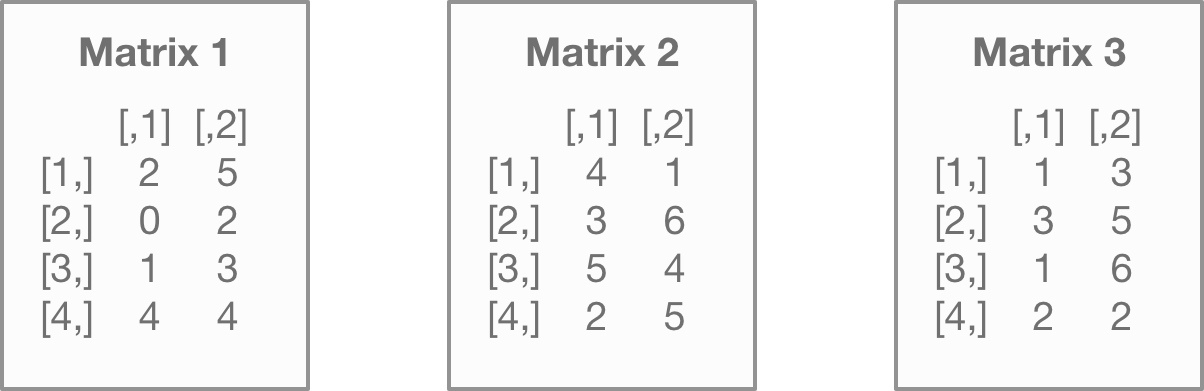
\includegraphics[width=50%%]{1.29_Arrays_Flat} \end{center}

And then stacks them into an array:


\begin{center}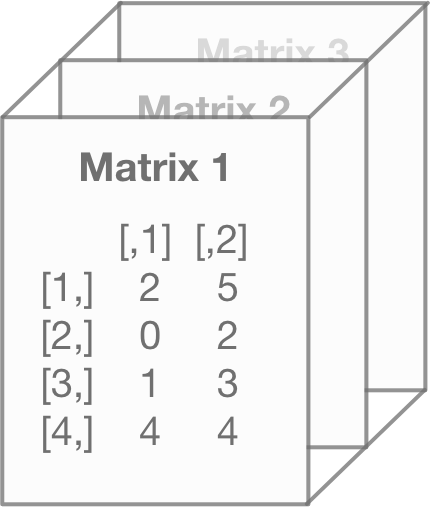
\includegraphics[width=0.15\linewidth]{1.30_Arrays_Stacked} \end{center}

You can then select the first and twenty-second entry with the scripts below.

\begin{Shaded}
\begin{Highlighting}[]
\NormalTok{array1[}\DecValTok{1}\NormalTok{]}
\end{Highlighting}
\end{Shaded}

\begin{verbatim}
## [1] 2
\end{verbatim}

\begin{Shaded}
\begin{Highlighting}[]
\NormalTok{array1[}\DecValTok{22}\NormalTok{]}
\end{Highlighting}
\end{Shaded}

\begin{verbatim}
## [1] 5
\end{verbatim}

To help you visualize this, I highlighted the fifth and twenty second values from the array in the illustration below:

\begin{center}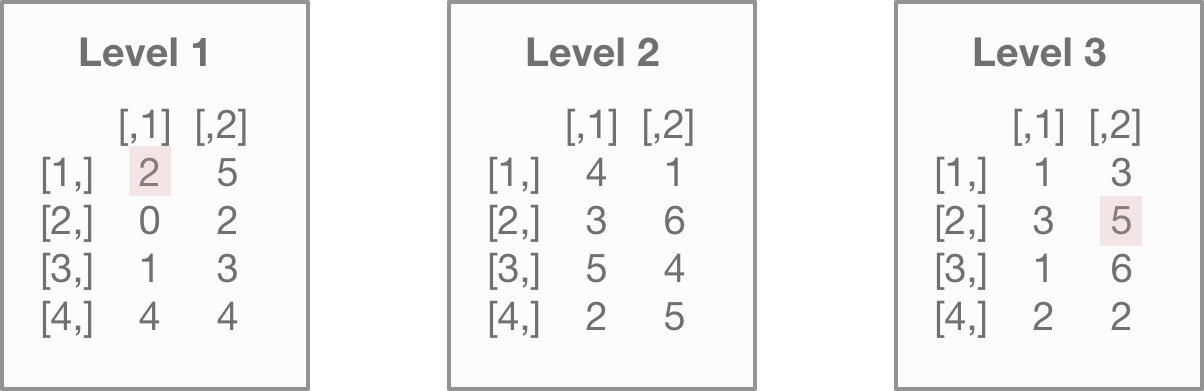
\includegraphics[width=0.5\linewidth]{1.35_Arrays_Highlight_1} \end{center}

With arrays, selecting particular columns or rows gets difficult because arrays can have multiple dimensions. That introduces the \texttt{{[}r,c,d{]}} notation.

Down below, we select the entire second row of every matrix in our array:

\begin{Shaded}
\begin{Highlighting}[]
\NormalTok{array1[}\DecValTok{2}\NormalTok{,,]}
\end{Highlighting}
\end{Shaded}

\begin{verbatim}
##      [,1] [,2] [,3]
## [1,]    0    3    3
## [2,]    2    6    5
\end{verbatim}

You may have noticed that this ``flipped'' the direction. R isn't trying to confuse you. It's merely displaying the previous, individual matrix rows as columns. So column 1 shows the results from matrix 1 in the previous array. Keep this in mind as you interact with arrays. The output may not always be intuitive.

Down below is an illustration of how R processes this command.

First, R finds the second row for each level of the array\ldots{}

\begin{center}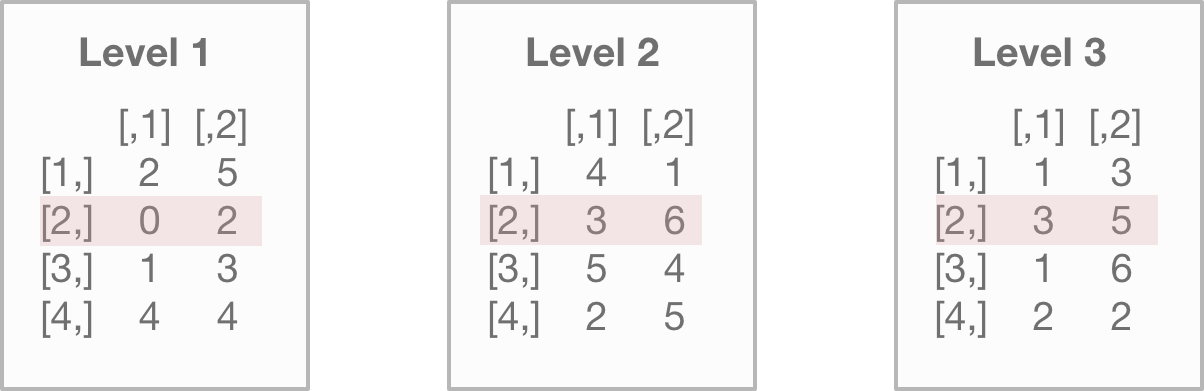
\includegraphics[width=0.5\linewidth]{1.36.1_Array_Row_Selection} \end{center}

And R then pivots and places those rows into a new array, with each column representing the level of the array\ldots{}

\begin{center}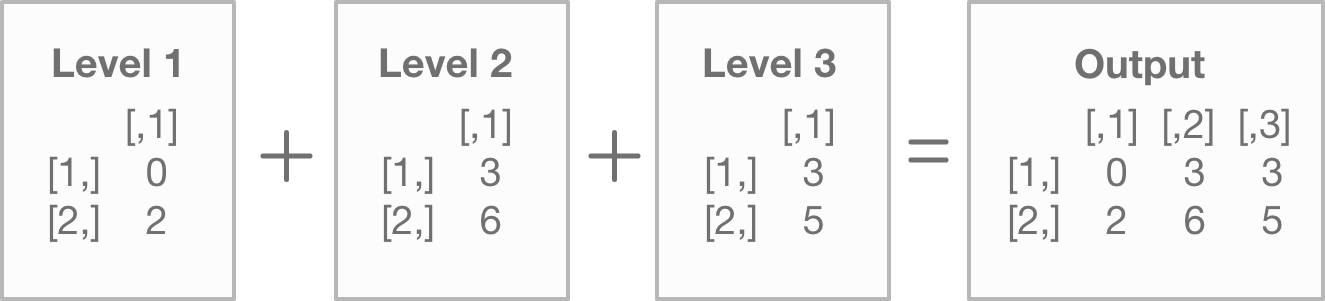
\includegraphics[width=0.65\linewidth]{1.36.2_Array_Row_Selection} \end{center}

Just like rows, we can also the second column of every matrix:

\begin{Shaded}
\begin{Highlighting}[]
\NormalTok{array1[,}\DecValTok{2}\NormalTok{,]}
\end{Highlighting}
\end{Shaded}

\begin{verbatim}
##      [,1] [,2] [,3]
## [1,]    5    1    3
## [2,]    2    6    5
## [3,]    3    4    6
## [4,]    4    5    2
\end{verbatim}

Down below is an illustration of how R processes this command. R takes the second column from each level of the array and outputs it. Each column of the output represents the level of the array.

\begin{center}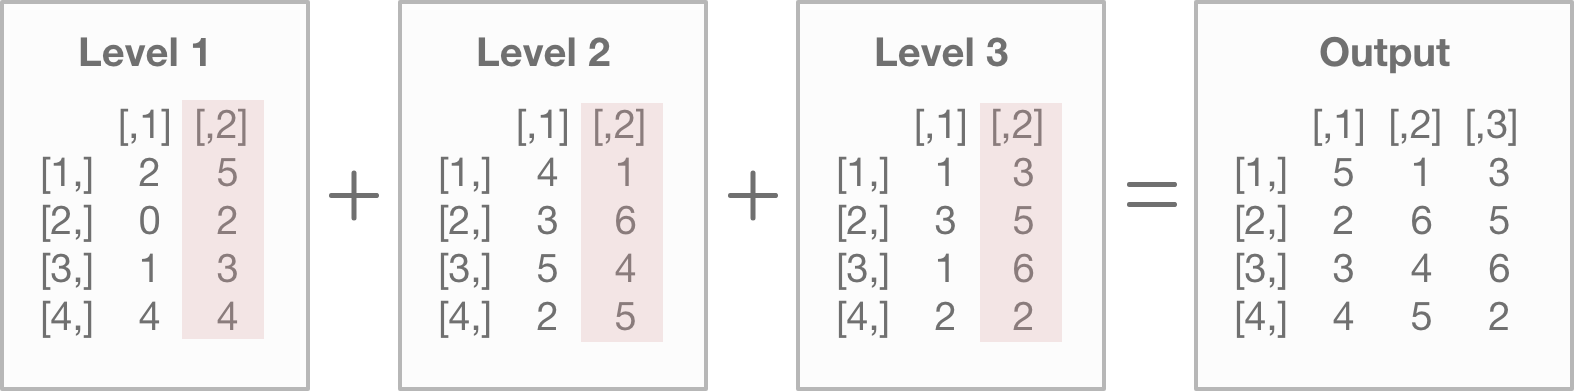
\includegraphics[width=0.7\linewidth]{1.37.1_Array_Column_Selection} \end{center}

We can also select every entry in the third matrix of our array:

\begin{Shaded}
\begin{Highlighting}[]
\NormalTok{array1[,,}\DecValTok{3}\NormalTok{]}
\end{Highlighting}
\end{Shaded}

\begin{verbatim}
##      [,1] [,2]
## [1,]    1    3
## [2,]    3    5
## [3,]    1    6
## [4,]    2    2
\end{verbatim}

We can even get a specific entry by selecting the second row, second column of the third matrix in our array:

\begin{Shaded}
\begin{Highlighting}[]
\NormalTok{array1[}\DecValTok{2}\NormalTok{,}\DecValTok{2}\NormalTok{,}\DecValTok{3}\NormalTok{]}
\end{Highlighting}
\end{Shaded}

\begin{verbatim}
## [1] 5
\end{verbatim}

You can transform arrays in the same way as the other objects. Down below are some examples of how we can use those same techniques. Copy and paste the code below to your own computer to get an idea of how this works.

\begin{Shaded}
\begin{Highlighting}[]
\NormalTok{array1 }
\CommentTok{#Changes the 2nd value of the entire array to a 2}
\NormalTok{array1[}\DecValTok{2}\NormalTok{] <-}\StringTok{ }\DecValTok{2}
\NormalTok{array1}
\CommentTok{#Changes the 2nd column of each matrix to a 2}
\NormalTok{array1[,}\DecValTok{2}\NormalTok{,] <-}\StringTok{ }\DecValTok{2}
\NormalTok{array1}
\CommentTok{#Changes the 2nd row, 1st column of the 3rd array to 0}
\NormalTok{array1[}\DecValTok{2}\NormalTok{,}\DecValTok{1}\NormalTok{,}\DecValTok{3}\NormalTok{] <-}\StringTok{ }\DecValTok{0}
\NormalTok{array1}
\CommentTok{#Divided the 3rd matrix only by 3}
\NormalTok{array1[,,}\DecValTok{3}\NormalTok{] <-}\StringTok{ }\NormalTok{array1[,,}\DecValTok{3}\NormalTok{] }\OperatorTok{/}\StringTok{ }\DecValTok{3}
\NormalTok{array1}
\end{Highlighting}
\end{Shaded}

\hypertarget{how-to-filter-and-transform-data-from-a-data-frame}{%
\section{How to Filter and Transform Data from a Data Frame}\label{how-to-filter-and-transform-data-from-a-data-frame}}

There's two approaches you can take to selecting data from a data frame. There's the ``classic'' approach, which I'll show you in this section, and then there's the \textbf{data plyer} approach.

The classic approach uses R base to interact with data frames. The data plyer approach uses a package called \texttt{dplyr} to transform the data. The \texttt{dplyr} syntax is far more readable, which is handy for really long scripts. I personally recommend the data plyer approach and will detail it in a chapter called \emph{How to Select and Transform Data Using the \texttt{dplyr} Package}.

If you don't want to confuse yourself by learning two different methods, feel free to skip this section and go to the chapter on \texttt{dplyr}. (Will be available in future versions). This section will show the classical approach.

Down below is a script to load the James Bond data frame from the last chapter:

\begin{Shaded}
\begin{Highlighting}[]
\NormalTok{bond <-}\StringTok{ }\KeywordTok{read.csv}\NormalTok{(}\StringTok{"https://raw.githubusercontent.com/taylorrodgers/bond/main/bond.csv"}\NormalTok{)}
\end{Highlighting}
\end{Shaded}

As you can see, a data frame is built using smaller vectors. This gives you a clue to how to select data.

For example, you can re-select individual vectors back out using the \texttt{\$} notation:

\begin{Shaded}
\begin{Highlighting}[]
\NormalTok{bond}\OperatorTok{$}\NormalTok{filmname}
\end{Highlighting}
\end{Shaded}

(Note: You'll need to run the scripts from this section on your own console. The output cannot fit cleanly on this pdf file.)

You can also produce a vector using the \texttt{{[},c{]}} notation. What this means is you're ignoring the row and selecting a column number. We generate the same result as our last section with this method.

\begin{Shaded}
\begin{Highlighting}[]
\NormalTok{bond[,}\DecValTok{1}\NormalTok{]}
\end{Highlighting}
\end{Shaded}

If you use the \texttt{{[}n{]}} notation, you'll select the same column as before, but you're keeping it in a data frame structure.

\begin{Shaded}
\begin{Highlighting}[]
\NormalTok{bond[}\DecValTok{1}\NormalTok{]}
\end{Highlighting}
\end{Shaded}

As you may have noticed, the \texttt{{[}n{]}} notation in this context works differently than other object types. For data frames, \texttt{{[}n{]}} selects the \emph{nth} column and NOT the \emph{nth} data entry.

You can use the \texttt{{[}n:n{]}} or the \texttt{{[},n:n{]}} notation to select multiple columns. Both will be presented as a data frame.

\begin{Shaded}
\begin{Highlighting}[]
\NormalTok{bond[}\DecValTok{1}\OperatorTok{:}\DecValTok{3}\NormalTok{]}
\NormalTok{bond[,}\DecValTok{1}\OperatorTok{:}\DecValTok{3}\NormalTok{]}
\end{Highlighting}
\end{Shaded}

To select an individual or range of rows, you use the same \texttt{{[}r,c{]}} notation as before:

\begin{Shaded}
\begin{Highlighting}[]
\NormalTok{bond[}\DecValTok{1}\OperatorTok{:}\DecValTok{3}\NormalTok{,] }\CommentTok{# Selects first three rows}
\end{Highlighting}
\end{Shaded}

\begin{verbatim}
##      filmname year        actor     gross
## 1     Skyfall 2012 Daniel Craig 1108.5610
## 2 Thunderball 1965 Sean Connery 1014.9411
## 3  Goldfinger 1964 Sean Connery  912.2575
\end{verbatim}

You can also exclude rows or columns using the negative \texttt{-} sign before the row or column numbers:

\begin{Shaded}
\begin{Highlighting}[]
\NormalTok{bond[}\OperatorTok{-}\DecValTok{1}\OperatorTok{:-}\DecValTok{20}\NormalTok{,] }\CommentTok{# Excludes rows 1 through 20}
\end{Highlighting}
\end{Shaded}

\begin{verbatim}
##                filmname year          actor    gross
## 21            Octopussy 1983    Roger Moore 426.2444
## 22 The Living Daylights 1987 Timothy Dalton 381.0889
## 23     A View to a Kill 1985    Roger Moore 321.1726
## 24      Licence to Kill 1989 Timothy Dalton 285.1572
\end{verbatim}

\begin{Shaded}
\begin{Highlighting}[]
\NormalTok{bond[}\DecValTok{3}\NormalTok{,}\OperatorTok{-}\DecValTok{4}\NormalTok{] }\CommentTok{# Row 3, excluding the 4th column}
\end{Highlighting}
\end{Shaded}

\begin{verbatim}
##     filmname year        actor
## 3 Goldfinger 1964 Sean Connery
\end{verbatim}

Just like the other object types, you can use logical and arithmetic operators, which makes it easy to filter to what you need. Note: this is where things start to get complicated with data frame filtering and why I suggest the \texttt{dplyr} package.

Lets say we want to filter by year. We want only Bond films made after 1990. First, we'll generate our TRUE / FALSE output. Go ahead and take the script below and run it in your own console:

\begin{Shaded}
\begin{Highlighting}[]
\NormalTok{bond[}\StringTok{"year"}\NormalTok{]}\OperatorTok{>=}\DecValTok{1990}
\end{Highlighting}
\end{Shaded}

Now, you'll notice that I intentionally kept this as a data frame object type. Had I used the \texttt{bond\$year} notation, it would've turned it into a vector. This would've made further filtering later more difficult.

Next, we need to plug this into another script:

\begin{Shaded}
\begin{Highlighting}[]
\NormalTok{bond[bond[}\StringTok{"year"}\NormalTok{]}\OperatorTok{>=}\DecValTok{1990}\NormalTok{]}
\end{Highlighting}
\end{Shaded}

\begin{verbatim}
##  [1] "Skyfall"                 "Spectre"                
##  [3] "Casino Royale"           "Quantum of Solace"      
##  [5] "Die Another Day"         "Goldeneye"              
##  [7] "The World is Not Enough" "Tomorrow Never Dies"    
##  [9] "2012"                    "2015"                   
## [11] "2006"                    "2008"                   
## [13] "2002"                    "1995"                   
## [15] "1999"                    "1997"                   
## [17] "Daniel Craig"            "Daniel Craig"           
## [19] "Daniel Craig"            "Daniel Craig"           
## [21] "Pierce Brosnan"          "Pierce Brosnan"         
## [23] "Pierce Brosnan"          "Pierce Brosnan"         
## [25] "1108.5610"               " 880.6692"              
## [27] " 669.7895"               " 622.2464"              
## [29] " 543.6396"               " 529.5487"              
## [31] " 491.6172"               " 478.9464"
\end{verbatim}

If you notice though, this doesn't cleanly give us the information we need.

We need to make sure we preserve the columns. We can do this by simply adding a comma and / or specifying the column numbers:

\begin{Shaded}
\begin{Highlighting}[]
\NormalTok{bond[bond[}\StringTok{"year"}\NormalTok{]}\OperatorTok{>=}\DecValTok{1990}\NormalTok{,] }\CommentTok{# Includes all columns}
\end{Highlighting}
\end{Shaded}

\begin{verbatim}
##                   filmname year          actor     gross
## 1                  Skyfall 2012   Daniel Craig 1108.5610
## 4                  Spectre 2015   Daniel Craig  880.6692
## 8            Casino Royale 2006   Daniel Craig  669.7895
## 11       Quantum of Solace 2008   Daniel Craig  622.2464
## 13         Die Another Day 2002 Pierce Brosnan  543.6396
## 14               Goldeneye 1995 Pierce Brosnan  529.5487
## 16 The World is Not Enough 1999 Pierce Brosnan  491.6172
## 18     Tomorrow Never Dies 1997 Pierce Brosnan  478.9464
\end{verbatim}

\begin{Shaded}
\begin{Highlighting}[]
\NormalTok{bond[bond[}\StringTok{"year"}\NormalTok{]}\OperatorTok{>=}\DecValTok{1990}\NormalTok{,}\DecValTok{1}\OperatorTok{:}\DecValTok{3}\NormalTok{] }\CommentTok{# Columns 1 through 3}
\end{Highlighting}
\end{Shaded}

\begin{verbatim}
##                   filmname year          actor
## 1                  Skyfall 2012   Daniel Craig
## 4                  Spectre 2015   Daniel Craig
## 8            Casino Royale 2006   Daniel Craig
## 11       Quantum of Solace 2008   Daniel Craig
## 13         Die Another Day 2002 Pierce Brosnan
## 14               Goldeneye 1995 Pierce Brosnan
## 16 The World is Not Enough 1999 Pierce Brosnan
## 18     Tomorrow Never Dies 1997 Pierce Brosnan
\end{verbatim}

\hypertarget{how-to-filter-a-list}{%
\section{How to Filter a List}\label{how-to-filter-a-list}}

Unlike the other object types, I won't go into detail about transforming a list. The reason is that lists are usually reserved as an output of various functions. Or they're a handy way of bunching other objects together. If you wanted to transform an object within a list, you'd probably transform that object directly.

Filtering a list is a useful skill to have though.

The script below creates a model using our James Bond data. That creates a \emph{list} of the various calculations in a regression analysis. The \texttt{names()} function then shows you all the objects contained within the list:

\begin{Shaded}
\begin{Highlighting}[]
\NormalTok{bondmodel <-}\StringTok{ }\KeywordTok{lm}\NormalTok{(gross }\OperatorTok{~}\StringTok{ }\NormalTok{actor,}\DataTypeTok{data=}\NormalTok{bond)}
\KeywordTok{names}\NormalTok{(bondmodel)}
\end{Highlighting}
\end{Shaded}

(Note: You'll need to run the scripts from this section on your own console. The output cannot fit cleanly on this pdf file.)

We can select any of these objects within the list with the \texttt{\$}, \texttt{{[}"object\_name"{]}}, or \texttt{{[}n{]}} notations:

\begin{Shaded}
\begin{Highlighting}[]
\NormalTok{bondmodel}\OperatorTok{$}\NormalTok{coefficients}
\NormalTok{bondmodel[}\StringTok{"coefficients"}\NormalTok{]}
\NormalTok{bondmodel[}\DecValTok{1}\NormalTok{]}
\end{Highlighting}
\end{Shaded}

Now here's where things get tricky. Let's say we want to filter down to a smaller value within the objects of the list. That changes depending on those object types. Confused?

It's better if we go with a simpler example than the list generated by the \texttt{lm()} function.

Down below, I create a list using some of the other objects we made in this lesson:

\begin{Shaded}
\begin{Highlighting}[]
\NormalTok{v1 <-}\StringTok{ }\KeywordTok{c}\NormalTok{(}\OtherTok{TRUE}\NormalTok{,}\OtherTok{FALSE}\NormalTok{,}\OtherTok{TRUE}\NormalTok{)}
\NormalTok{v2 <-}\StringTok{ }\KeywordTok{c}\NormalTok{(}\StringTok{"Hola"}\NormalTok{,}\StringTok{"Howdy"}\NormalTok{,}\StringTok{"Hello"}\NormalTok{)}
\NormalTok{v3 <-}\StringTok{ }\KeywordTok{c}\NormalTok{(}\DecValTok{1}\OperatorTok{:}\DecValTok{3}\NormalTok{)}
\NormalTok{list1 <-}\StringTok{ }\KeywordTok{list}\NormalTok{(}\DataTypeTok{vector1=}\NormalTok{v1,}
              \DataTypeTok{vector2=}\NormalTok{v2,}
              \DataTypeTok{vector3=}\NormalTok{v3,}
              \DataTypeTok{matrix1=}\NormalTok{matrix1,}
              \DataTypeTok{array1=}\NormalTok{array1,}
              \DataTypeTok{bond=}\NormalTok{bond)}
\end{Highlighting}
\end{Shaded}

I can select any one of those objects from the list using the \texttt{\$} notation:

\begin{Shaded}
\begin{Highlighting}[]
\NormalTok{list1}\OperatorTok{$}\NormalTok{vector1}
\end{Highlighting}
\end{Shaded}

\begin{verbatim}
## [1]  TRUE FALSE  TRUE
\end{verbatim}

\begin{Shaded}
\begin{Highlighting}[]
\NormalTok{list1}\OperatorTok{$}\NormalTok{matrix1}
\end{Highlighting}
\end{Shaded}

\begin{verbatim}
##      [,1] [,2]
## [1,]    2    1
## [2,]    0    3
\end{verbatim}

Now let's say I want to select a specific data point from the list. Let's say I want to know the Bond actors. I know that information was stored within a data frame within the list. To pull that data, I use a combination of filtering techniques.

First, I have to pull the data frame from the list. I do that with the \texttt{\$} notation. Then, we treat the object type as a normal data frame.

Here's what I mean:

\begin{Shaded}
\begin{Highlighting}[]
\NormalTok{list1}\OperatorTok{$}\NormalTok{bond[}\DecValTok{3}\NormalTok{]}
\NormalTok{list1}\OperatorTok{$}\NormalTok{bond}\OperatorTok{$}\NormalTok{actor}
\NormalTok{list1}\OperatorTok{$}\NormalTok{bond[}\StringTok{"actor"}\NormalTok{]}
\end{Highlighting}
\end{Shaded}

I do the same with the other object types here:

\begin{Shaded}
\begin{Highlighting}[]
\NormalTok{list1}\OperatorTok{$}\NormalTok{vector1[}\DecValTok{3}\NormalTok{]}
\end{Highlighting}
\end{Shaded}

\begin{verbatim}
## [1] TRUE
\end{verbatim}

\begin{Shaded}
\begin{Highlighting}[]
\NormalTok{list1}\OperatorTok{$}\NormalTok{vector3[v3}\OperatorTok{>=}\DecValTok{2}\NormalTok{]}
\end{Highlighting}
\end{Shaded}

\begin{verbatim}
## [1] 2 3
\end{verbatim}

\begin{Shaded}
\begin{Highlighting}[]
\NormalTok{list1}\OperatorTok{$}\NormalTok{array1[,}\DecValTok{2}\NormalTok{,]}
\end{Highlighting}
\end{Shaded}

\begin{verbatim}
##      [,1] [,2]      [,3]
## [1,]    2    2 0.6666667
## [2,]    2    2 0.6666667
## [3,]    2    2 0.6666667
## [4,]    2    2 0.6666667
\end{verbatim}

\hypertarget{things-to-remember-3}{%
\section{Things to Remember}\label{things-to-remember-3}}

\begin{itemize}
\tightlist
\item
  How you filter and transform data depends upon the object type
\end{itemize}

\hypertarget{exercises}{%
\section{Exercises}\label{exercises}}

Try to see if you can complete the following exercises. Answers are in the back of the book!

\begin{enumerate}
\def\labelenumi{\arabic{enumi}.}
\tightlist
\item
  Filter the following vector to values greater than 2. Display the actual number (not TRUE / FALSE).
\end{enumerate}

\begin{Shaded}
\begin{Highlighting}[]
\NormalTok{q1 <-}\StringTok{ }\KeywordTok{seq}\NormalTok{(}\DecValTok{1}\NormalTok{,}\DecValTok{20}\NormalTok{,}\DecValTok{2}\NormalTok{)}
\end{Highlighting}
\end{Shaded}

\begin{enumerate}
\def\labelenumi{\arabic{enumi}.}
\setcounter{enumi}{1}
\tightlist
\item
  Filter the following vector to values between 19 and 20, but only for the first three entries that meet that criteria. (Hint: add \texttt{{[}n:n{]}} for the range of values after you determine which values meet that criteria)
\end{enumerate}

\begin{Shaded}
\begin{Highlighting}[]
\NormalTok{q2 <-}\StringTok{ }\KeywordTok{round}\NormalTok{(}\KeywordTok{rnorm}\NormalTok{(}\DecValTok{20}\NormalTok{,}\DecValTok{32}\NormalTok{,}\DecValTok{7}\NormalTok{),}\DecValTok{0}\NormalTok{)}
\end{Highlighting}
\end{Shaded}

\begin{enumerate}
\def\labelenumi{\arabic{enumi}.}
\setcounter{enumi}{2}
\tightlist
\item
  Multiple the following matrices together.
\end{enumerate}

\begin{Shaded}
\begin{Highlighting}[]
\NormalTok{q3_}\DecValTok{1}\NormalTok{ <-}\StringTok{ }\KeywordTok{matrix}\NormalTok{(}\KeywordTok{round}\NormalTok{(}\KeywordTok{seq}\NormalTok{(}\DecValTok{1}\NormalTok{,}\DecValTok{40}\NormalTok{,}\FloatTok{3.27}\NormalTok{),}\DecValTok{0}\NormalTok{),}\DecValTok{3}\NormalTok{)}
\NormalTok{q3_}\DecValTok{2}\NormalTok{ <-}\StringTok{ }\KeywordTok{matrix}\NormalTok{(}\KeywordTok{seq}\NormalTok{(}\DecValTok{1}\NormalTok{,}\DecValTok{8}\NormalTok{,}\DecValTok{1}\NormalTok{),}\DecValTok{4}\NormalTok{)}
\end{Highlighting}
\end{Shaded}

\begin{enumerate}
\def\labelenumi{\arabic{enumi}.}
\setcounter{enumi}{3}
\tightlist
\item
  Subtract 41 from every entry in the second column of the following matrix. Replace the column with those new values.
\end{enumerate}

\begin{Shaded}
\begin{Highlighting}[]
\NormalTok{q4 <-}\StringTok{ }\KeywordTok{matrix}\NormalTok{(}\KeywordTok{seq}\NormalTok{(}\DecValTok{1}\NormalTok{,}\DecValTok{120}\NormalTok{,}\DecValTok{4}\NormalTok{),}\DecValTok{10}\NormalTok{,}\DecValTok{3}\NormalTok{)}
\end{Highlighting}
\end{Shaded}

\begin{enumerate}
\def\labelenumi{\arabic{enumi}.}
\setcounter{enumi}{4}
\tightlist
\item
  Select the second row from each matrix in the following array. Subtract 5 from those rows.
\end{enumerate}

\begin{Shaded}
\begin{Highlighting}[]
\NormalTok{q5 <-}\StringTok{ }\KeywordTok{array}\NormalTok{(}\DataTypeTok{data=}\KeywordTok{c}\NormalTok{(}\KeywordTok{matrix}\NormalTok{(}\KeywordTok{seq}\NormalTok{(}\DecValTok{1}\NormalTok{,}\DecValTok{15}\NormalTok{,}\DecValTok{1}\NormalTok{),}\DecValTok{5}\NormalTok{,}\DecValTok{3}\NormalTok{),}
                  \KeywordTok{matrix}\NormalTok{(}\KeywordTok{seq}\NormalTok{(}\DecValTok{4}\NormalTok{,}\DecValTok{60}\NormalTok{,}\DecValTok{4}\NormalTok{),}\DecValTok{5}\NormalTok{,}\DecValTok{3}\NormalTok{),}
                  \KeywordTok{matrix}\NormalTok{(}\KeywordTok{seq}\NormalTok{(}\DecValTok{2}\NormalTok{,}\DecValTok{30}\NormalTok{,}\DecValTok{2}\NormalTok{),}\DecValTok{5}\NormalTok{,}\DecValTok{3}\NormalTok{)),}
            \DataTypeTok{dim=}\KeywordTok{c}\NormalTok{(}\DecValTok{5}\NormalTok{,}\DecValTok{3}\NormalTok{,}\DecValTok{3}\NormalTok{))}
\end{Highlighting}
\end{Shaded}

\begin{enumerate}
\def\labelenumi{\arabic{enumi}.}
\setcounter{enumi}{5}
\tightlist
\item
  Filter the James Bond data frame to only films starring Roger Moore.
\end{enumerate}

\begin{Shaded}
\begin{Highlighting}[]
\NormalTok{bond}
\end{Highlighting}
\end{Shaded}

\begin{enumerate}
\def\labelenumi{\arabic{enumi}.}
\setcounter{enumi}{6}
\tightlist
\item
  Filter the James Bond data frame to films starring Sean Connery made after 1966.
\end{enumerate}

\begin{Shaded}
\begin{Highlighting}[]
\NormalTok{bond}
\end{Highlighting}
\end{Shaded}

\hypertarget{dplyr}{%
\chapter{How to Filter and Transform Data with the Dplyr Package}\label{dplyr}}

In the last chapter, I showed you how to use R base to filter and transform data. Personally, I still think this is the best way to manage data in R. However, there's another popular package for data filtering and transformation -- the \texttt{dplyr} package.

The \texttt{dplyr} package (pronounced like ``data plier'') was developed by Hadley Wickham to allow more intuitive data transformation. It falls under the tidyverse packages, which includes other popular R packages created by Mr.~Wickham.

\hypertarget{why-is-dplyr-so-popular}{%
\section{\texorpdfstring{Why is \texttt{dplyr} So Popular?}{Why is dplyr So Popular?}}\label{why-is-dplyr-so-popular}}

\texttt{dplyr} is popular for its intuitive syntax for filtering and transforming data frames. If your programming background is with SQL, you'll find it an easier transition to make.

\texttt{dplyr} is also highly readable compared to base R. That's where I see the most value in it. You can send it over to another programmer and it'll be easier for them to read what you're doing with the data.

\hypertarget{its-still-worth-learning-base-r}{%
\section{It's Still Worth Learning Base R}\label{its-still-worth-learning-base-r}}

\texttt{dplyr}'s strengths are mostly limited to data frames, whereas base R can work with vectors, matrices, arrays, and lists. That makes it still worthwhile to study base R.

This isn't a knock against \texttt{dplyr}. Much of the work you'll do requires a data frame and most R functions work with data frames fairly easily. But writing your own functions should be done with base R.

\hypertarget{the-dplyr-syntax}{%
\section{\texorpdfstring{The \texttt{dplyr} Syntax}{The dplyr Syntax}}\label{the-dplyr-syntax}}

If you recall, filtering a data frame in base R looks like this:

\begin{Shaded}
\begin{Highlighting}[]
\CommentTok{#If needed, you can reload the Bond data set with this script}
\NormalTok{bond <-}\StringTok{ }\KeywordTok{read.csv}\NormalTok{(}\StringTok{"https://raw.githubusercontent.com/taylorrodgers/bond/main/bond.csv"}\NormalTok{)}

\NormalTok{bond[bond[}\StringTok{"year"}\NormalTok{]}\OperatorTok{>=}\DecValTok{1990}\NormalTok{,}\DecValTok{1}\OperatorTok{:}\DecValTok{3}\NormalTok{]}
\end{Highlighting}
\end{Shaded}

That's different in \texttt{dplyr}, which looks like this:

\begin{Shaded}
\begin{Highlighting}[]
\NormalTok{bond }\OperatorTok\StringTok{ }\KeywordTok{select}\NormalTok{(filmname,year,actor) }\OperatorTok\StringTok{ }\KeywordTok{filter}\NormalTok{(year}\OperatorTok{>=}\DecValTok{1990}\NormalTok{)}
\end{Highlighting}
\end{Shaded}

You can literally think of the \texttt{dplyr} syntax as a set of instructions to read one-by-one:

\begin{enumerate}
\def\labelenumi{\arabic{enumi}.}
\tightlist
\item
  Hey data set named ``Bond''\ldots{} \texttt{bond\ \%\textgreater{}\%}
\item
  Tell me the film name, year released, and actor name for\ldots{} \texttt{select(filmname,year,actor)\ \%\textgreater{}\%}
\item
  James Bond films made after 1990 \texttt{filter(year\textgreater{}=1990)}
\end{enumerate}

That's a lot easier to understand than normal base R, ain't it?

\hypertarget{understand-the-difference-between-selecting-and-filtering}{%
\section{Understand the Difference Between Selecting and Filtering}\label{understand-the-difference-between-selecting-and-filtering}}

With \texttt{dplyr}, it's important to remember the difference between selecting and filtering.

Selecting uses the \texttt{select()} function and reduces the \textbf{columns} to those you specify:

In addition to \texttt{select()}, there's also \texttt{mutate()} and \texttt{transmute()}, which serve similar purposes. We'll cover those two functions in the next section.

Filtering uses the \texttt{filter()} function and reduces the rows to those you specify.

\hypertarget{how-to-select-and-mutate-a-data-frame-with-dplyr-in-r}{%
\section{\texorpdfstring{How to Select and Mutate a Data Frame with \texttt{dplyr} in R}{How to Select and Mutate a Data Frame with dplyr in R}}\label{how-to-select-and-mutate-a-data-frame-with-dplyr-in-r}}

In dplyr, you can select columns using the \texttt{select()} function:

\begin{Shaded}
\begin{Highlighting}[]
\NormalTok{bond }\OperatorTok\StringTok{ }\KeywordTok{select}\NormalTok{(actor,filmname,gross)}
\end{Highlighting}
\end{Shaded}

Executing the code above will only select the columns \emph{actor}, \emph{filmname}, and \emph{gross.}

Sometimes you'll need to transform or alter the data. That's where \texttt{mutate()} comes in handy. \texttt{mutate()} will allow you to create new fields that alter existing ones. Confused?

Execute the script below to see:

\begin{Shaded}
\begin{Highlighting}[]
\NormalTok{bond }\OperatorTok\StringTok{ }\KeywordTok{mutate}\NormalTok{(}\DataTypeTok{gross_millions=}\NormalTok{gross}\OperatorTok{*}\DecValTok{1000000}\NormalTok{)}
\end{Highlighting}
\end{Shaded}

The \texttt{mutate()} function added a new column to the end called \emph{gross\_millions} with our new calculation.

The one drawback to \texttt{mutate()} is that it allow you to select specified columns. Rather than add another \texttt{\%\textgreater{}\%\ select()} to your code, you can use the \texttt{transmute()} function. \texttt{transmute()} basically combines the functionality of \texttt{mutate()} and \texttt{select()}. You can both define the columns you want to keep and mutate others.

\begin{Shaded}
\begin{Highlighting}[]
\NormalTok{bond }\OperatorTok\StringTok{ }\KeywordTok{transmute}\NormalTok{(actor,filmname,}\DataTypeTok{gross=}\NormalTok{gross}\OperatorTok{*}\DecValTok{1000000}\NormalTok{)}
\end{Highlighting}
\end{Shaded}

I personally like \texttt{transmute()} for selecting columns. However, \texttt{select()} and \texttt{mutate()} are appropriate in some situations.

\hypertarget{how-to-filter-a-data-frame-with-dplyr-in-r}{%
\section{\texorpdfstring{How to Filter a Data Frame with \texttt{dplyr} in R}{How to Filter a Data Frame with dplyr in R}}\label{how-to-filter-a-data-frame-with-dplyr-in-r}}

To filter rows in a data frame, use the \texttt{filter()} function:

\begin{Shaded}
\begin{Highlighting}[]
\NormalTok{bond }\OperatorTok\StringTok{ }\KeywordTok{filter}\NormalTok{(year}\OperatorTok{>=}\DecValTok{1980} \OperatorTok{&}\StringTok{ }\NormalTok{actor}\OperatorTok{==}\StringTok{"Daniel Craig"}\NormalTok{)}
\end{Highlighting}
\end{Shaded}

If you noticed, we used the same operators as in base R. We can use any R operators as below:

\begin{table}

\caption{\label{tab:dplyr-fig8}R Operators}
\centering
\begin{tabular}[t]{ll}
\toprule
label & symbol\\
\midrule
less than & <\\
greater than & >\\
less than or equal & <=\\
greater than or equal & >=\\
equal & ==\\
\addlinespace
does not equal & !=\\
and & \&\\
or & |\\
in & \%in\%\\
\bottomrule
\end{tabular}
\end{table}

You can apply any of these operators the \texttt{filter()} function:

\begin{Shaded}
\begin{Highlighting}[]
\NormalTok{bond }\OperatorTok\StringTok{ }\KeywordTok{filter}\NormalTok{(actor }\OperatorTok{==}\StringTok{ "Daniel Craig"} \OperatorTok{|}\StringTok{ }\NormalTok{actor }\OperatorTok{==}\StringTok{ "Sean Connery"}\NormalTok{)}
\NormalTok{bond }\OperatorTok\StringTok{ }\KeywordTok{filter}\NormalTok{(gross }\OperatorTok{>=}\StringTok{ }\DecValTok{700} \OperatorTok{&}\StringTok{ }\NormalTok{year }\OperatorTok{<}\StringTok{ }\DecValTok{2000}\NormalTok{)}
\end{Highlighting}
\end{Shaded}

Like in base R, you can also pass vectors in for dynamic filters:

\begin{Shaded}
\begin{Highlighting}[]
\NormalTok{actor_list <-}\StringTok{ }\KeywordTok{c}\NormalTok{(}\StringTok{"Daniel Craig"}\NormalTok{,}\StringTok{"Sean Connery"}\NormalTok{,}\StringTok{"Timothy Dalton"}\NormalTok{)}
\NormalTok{bond }\OperatorTok\StringTok{ }\KeywordTok{filter}\NormalTok{(actor }\OperatorTok\StringTok{ }\NormalTok{actor_list)}
\end{Highlighting}
\end{Shaded}

\hypertarget{how-to-summarize-and-group-data-with-dplyr-in-r}{%
\section{\texorpdfstring{How to Summarize and Group Data with \texttt{dplyr} in R}{How to Summarize and Group Data with dplyr in R}}\label{how-to-summarize-and-group-data-with-dplyr-in-r}}

Probably the most useful thing about \texttt{dplyr} is the ability to create new data frames that group and summarize data found in the larger data set. This is the primary reason I like \texttt{dplyr}.

Let's say you wanted to take the Bond data set and find out the gross revenue mean and standard deviation for Daniel Craig and Sean Connery. To accomplish this in base R, you'd have to use the following code:

\begin{Shaded}
\begin{Highlighting}[]
\KeywordTok{data.frame}\NormalTok{(}\DataTypeTok{actor_subselect=}\KeywordTok{c}\NormalTok{(}\StringTok{"Daniel Craig"}\NormalTok{,}\StringTok{"Sean Connery"}\NormalTok{), }
           \DataTypeTok{average_revenue=}\KeywordTok{c}\NormalTok{(}\KeywordTok{mean}\NormalTok{(bond[bond}\OperatorTok{$}\NormalTok{actor}\OperatorTok{==}\StringTok{"Daniel Craig"}\NormalTok{,}\StringTok{"gross"}\NormalTok{]),}
                             \KeywordTok{mean}\NormalTok{(bond[bond}\OperatorTok{$}\NormalTok{actor}\OperatorTok{==}\StringTok{"Sean Connery"}\NormalTok{,}\StringTok{"gross"}\NormalTok{])),}
           \DataTypeTok{sdev_revenue=}\KeywordTok{c}\NormalTok{(}\KeywordTok{sd}\NormalTok{(bond[bond}\OperatorTok{$}\NormalTok{actor}\OperatorTok{==}\StringTok{"Daniel Craig"}\NormalTok{,}\StringTok{"gross"}\NormalTok{]),}
                          \KeywordTok{sd}\NormalTok{(bond[bond}\OperatorTok{$}\NormalTok{actor}\OperatorTok{==}\StringTok{"Sean Connery"}\NormalTok{,}\StringTok{"gross"}\NormalTok{])))}
\end{Highlighting}
\end{Shaded}

It's not very simple, is it? Imagine having to do that for a much larger data set with even more actors!

\texttt{dplyr}'s \texttt{group\_by()} and \texttt{summarize()} functions really cut down on this work. Here's how we can accomplish the same thing as above:

\begin{Shaded}
\begin{Highlighting}[]
\NormalTok{bond }\OperatorTok\StringTok{ }\KeywordTok{filter}\NormalTok{(actor}\OperatorTok{==}\StringTok{"Daniel Craig"} \OperatorTok{|}\StringTok{ }\NormalTok{actor }\OperatorTok{==}\StringTok{ "Sean Connery"}\NormalTok{) }\OperatorTok\StringTok{ }
\StringTok{        }\KeywordTok{group_by}\NormalTok{(actor) }\OperatorTok\StringTok{ }
\StringTok{        }\KeywordTok{summarize}\NormalTok{(}\DataTypeTok{average_revenue=}\KeywordTok{mean}\NormalTok{(gross),}\DataTypeTok{sdev_revenue=}\KeywordTok{sd}\NormalTok{(gross))}
\end{Highlighting}
\end{Shaded}

Now you'll notice this script isn't shorter than what we did earlier. However, it's a lot easier to read. That's the beauty of \texttt{dplyr}!

\hypertarget{things-to-remember-4}{%
\section{Things to Remember}\label{things-to-remember-4}}

\begin{itemize}
\tightlist
\item
  \texttt{dplyr} is a package that provides a more intuitive syntax for transforming and analyzing data frames in R
\item
  Select and create new columns with \texttt{select()}, \texttt{mutate()}, and \texttt{transmute()}
\item
  Filter rows with \texttt{filter()} and the base R operators
\item
  Provide summary statistics with \texttt{group\_by()} and \texttt{summarize()} functions
\end{itemize}

\hypertarget{packages}{%
\chapter{Understanding and Using R Packages}\label{packages}}

Packages are one of the most important concepts in R programming. It's almost hard to conceive R programming without them.

An R \textbf{package} stores various functions and data sets for other users to access. It allows R to move beyond its roots in statistical programming and achieve more complex goals.

For example, you might be writing a research paper. You want to clearly show the results of your regression analysis in this report, along with various tables and charts. You can use a combination of \emph{Rmarkdown}, \emph{ggplot2}, \emph{xtable}, and various other packages to accomplish this goal.

That way you don't have to copy and paste your work to a word document as you analyze the results. You merely write it and program it in R and then export it to Word when you're done. This saves you a lot of time in the long run and makes your code far more re-producible.

\hypertarget{why-does-r-use-packages}{%
\section{Why Does R Use Packages?}\label{why-does-r-use-packages}}

Packages allow R to operate as an open source language. Programmers, statisticians, and data scientists can develop new functions and commands and then share them with other users elsewhere - for free! This is common for open source programming languages.

If you want, you can actually develop you're own package. If you find existing resources don't perform or operate the way you'd like, you can develop your own functions and save them in a package for others to use.

\hypertarget{how-to-access-r-packages}{%
\section{How to Access R Packages}\label{how-to-access-r-packages}}

Before I show you how to use an R package, you need to understand there's a difference between \textbf{installing} and \textbf{loading} a package. Installing means pulling it from CRAN and saving it on your computer. Loading a package means using it in your current R session.

Why would R do this?

Mostly for efficiency. It would take more memory if your R session ran every package installed on your computer. It improves your computer's performance to load packages only as you need them.

Also, it's not uncommon for R packages from different developers to have functions with the same name, but different purposes and inputs. Forcing you to load only the package with the function solves this issue.

\hypertarget{how-to-install-and-load-a-package---the-easy-way}{%
\section{How to Install and Load a Package - The Easy Way}\label{how-to-install-and-load-a-package---the-easy-way}}

There are a couple of different ways to install and load packages. It depends on whether you need to save and re-use your code later or if you're running a quick analysis.

The easiest way to manage R packages is through RStudio's user interface. This is better for quick analysis that you don't need to save.

The RStudio packages tab on the bottom right pane neatly organizes and details your current packages:

\begin{center}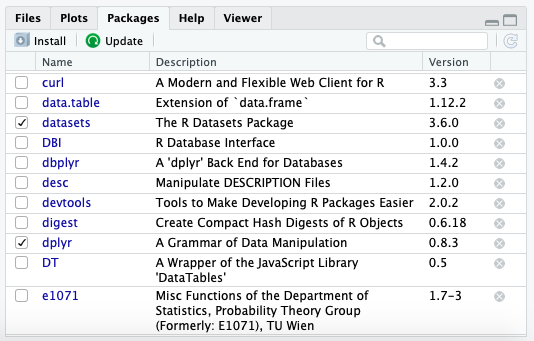
\includegraphics[width=0.6\linewidth]{1.24_Packages} \end{center}

You can use this tab to install and download a package.

To install a package, select the install button:

\begin{center}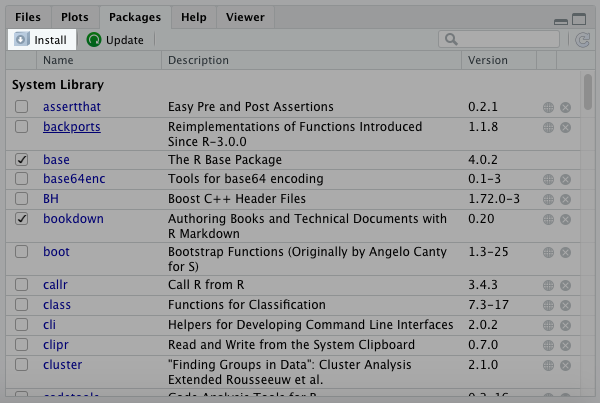
\includegraphics[width=0.6\linewidth]{1.38_Install_Package} \end{center}

After that, type in the name of your package. In the example below, I type in ``dplyr'' to install the \texttt{dplyr} package.

\begin{center}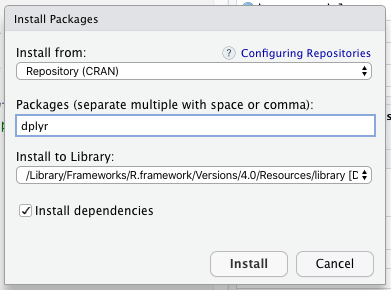
\includegraphics[width=0.6\linewidth]{1.39_Install_Dplyr} \end{center}

You will now see this package show up in the packages tab in the bottom right pane of RStudio:

\begin{center}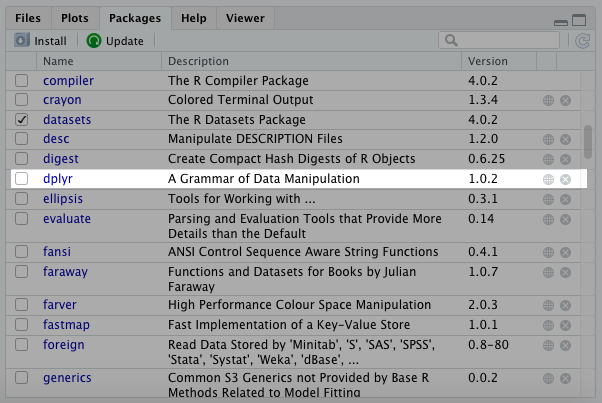
\includegraphics[width=0.6\linewidth]{1.40_Dplyr_Package} \end{center}

This doesn't make the dplyr package available for us to use though. We still have to \emph{load} it.

This is where RStudio makes things easy. All you have to do is click the little check box next to \textbf{dplyr} to load it.

\begin{center}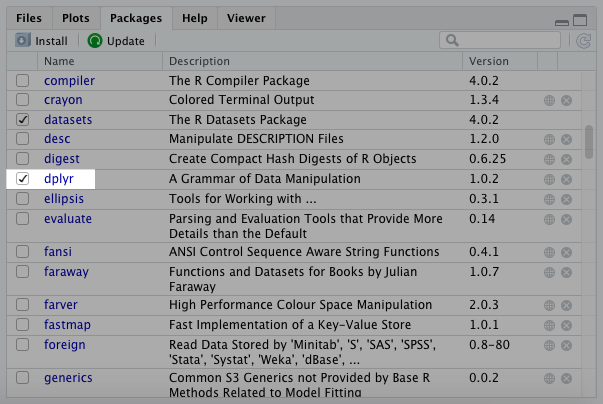
\includegraphics[width=0.6\linewidth]{1.41_Dplyr_Loaded} \end{center}

And now your package is loaded!

\hypertarget{why-you-should-still-learn-to-install-and-load-packages-the-old-fashioned-way}{%
\section{Why You Should Still Learn to Install and Load Packages the ``Old Fashioned'' Way}\label{why-you-should-still-learn-to-install-and-load-packages-the-old-fashioned-way}}

A developer once told me people who use RStudio weren't real ``programmers.'' Real programmers, he said, type everything out by hand. RStudio was for ``posers.''

If that's true, I am happy to be a poser. RStudio makes package management far easier. But there are some legitimate reasons to use the old fashioned methods, other than proving yourself as a real programmer.

If you need to share your code with other people, for example, it's better to include any code that installs and / or loads packages needed. That way the person opening your script doesn't have to guess which packages to load.

\hypertarget{how-to-install-and-load-r-packages---the-old-fashioned-way}{%
\section{How to Install and Load R Packages - The Old Fashioned Way}\label{how-to-install-and-load-r-packages---the-old-fashioned-way}}

There are two key functions you need to remember to install and load a package:
1. \texttt{install.packages()}
2. \texttt{library()}

\texttt{install.packages()} installs the package from CRAN onto your computer. \texttt{library()} will load it into your current R session.

Oddly enough, there's a difference in notation between the two. The \texttt{install.packages()} function requires you to put quotations "" around the package name. \texttt{library()} does not.

To see what I mean, look at the example down below:

\begin{Shaded}
\begin{Highlighting}[]
  \KeywordTok{install.packages}\NormalTok{(}\StringTok{"dplyr"}\NormalTok{)}
  \KeywordTok{library}\NormalTok{(dplyr)}
\end{Highlighting}
\end{Shaded}

Notice how the quotations marks are used in the first function? This is required for \texttt{install.packages()}. The \texttt{library()} function does not require it, but you can use quotation marks and it'll still execute.

\hypertarget{a-simple-trick-to-include-install-and-load-any-packages-needed}{%
\section{A Simple Trick to Include Install and Load Any Packages Needed}\label{a-simple-trick-to-include-install-and-load-any-packages-needed}}

If you share your R script with a colleague, they may not have all packages needed on their local computer to execute it.

To take care of this, you can include both the \texttt{install.packages()} and \texttt{library()} functions at the top of the script.

If it's a script that only you'll use in the future, you only need to include the \texttt{library()} function near the beginning, as you already installed the package beforehand.

\hypertarget{how-to-find-new-packages-to-install}{%
\section{How to Find New Packages to Install}\label{how-to-find-new-packages-to-install}}

One of the best kept secrets of computer engineers and programmers is that the majority of what they learned came from Google. Every time something doesn't work, they google how to do it.

Changes are high that you'll do the same as you program in R and most of these sites will tell you what packages to download. It's typically in the top left or right corner.

\begin{center}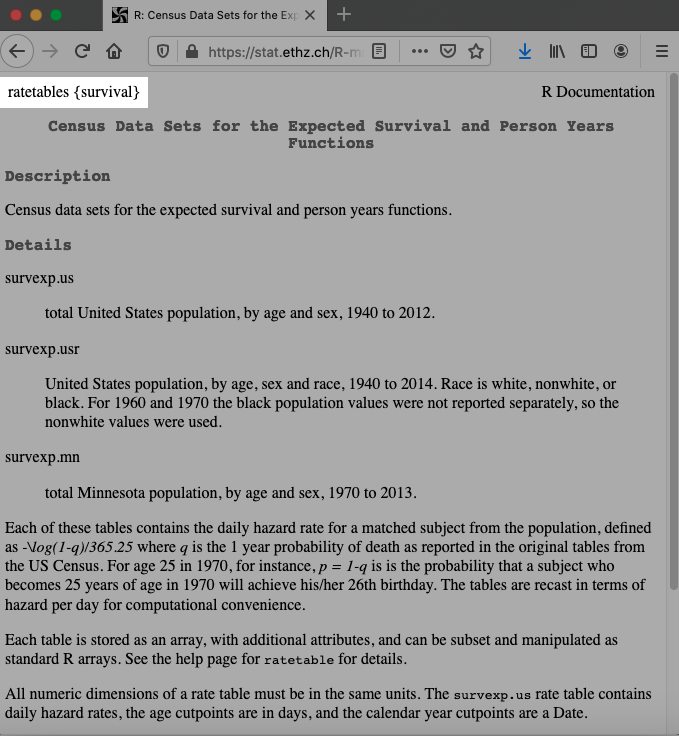
\includegraphics[width=0.6\linewidth]{1.42_Package_Info} \end{center}

For example, I recently google'd ``survival analysis in R.'' Unlike regression analysis, R doesn't have handy base functions to perform survival analysis. I found a couple of websites with information on how to do this in R. All of them required a new package called \textbf{survival}, which they displayed in the top left or right of the website.

\begin{center}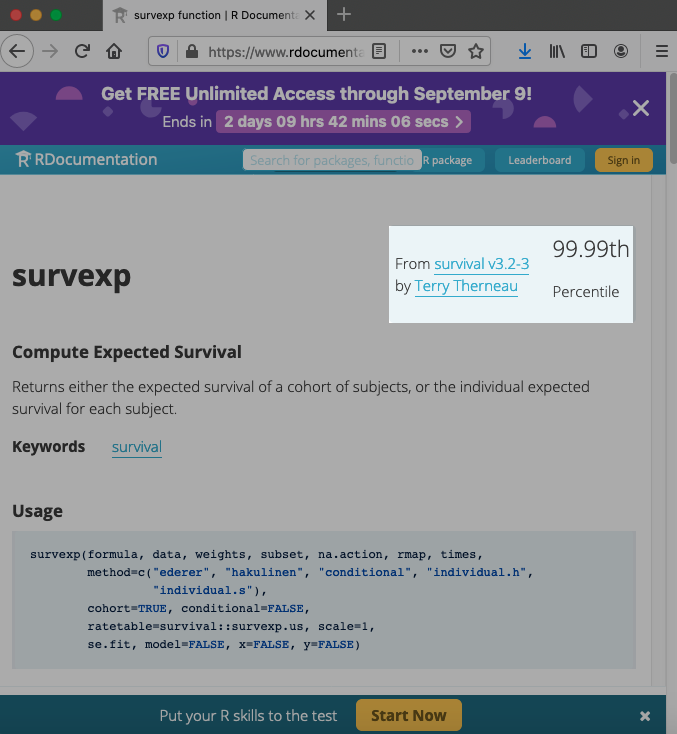
\includegraphics[width=0.6\linewidth]{1.43_Package_Info} \end{center}

\hypertarget{how-to-find-documentation-on-packages}{%
\section{How to Find Documentation on Packages}\label{how-to-find-documentation-on-packages}}

Most packages you install will have documentation with it. Sadly, much of this documentation is unreadable, but it's still a great resource and I rely on it heavily.

To access this documentation, you can click on the hyperlinked package name in the packages tab.

Click on the \textbf{dplyr} link on your own RStudio screen to see what I mean:

\begin{center}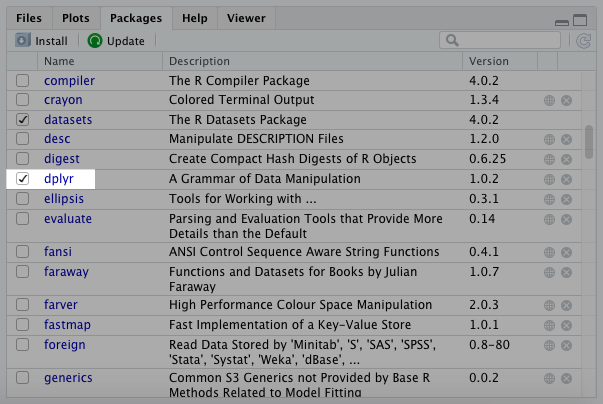
\includegraphics[width=0.6\linewidth]{1.41_Dplyr_Loaded} \end{center}

This will take you to the \textbf{Help} tab and you can see documentation on all commands, functions, and data sets for a given package.

\begin{center}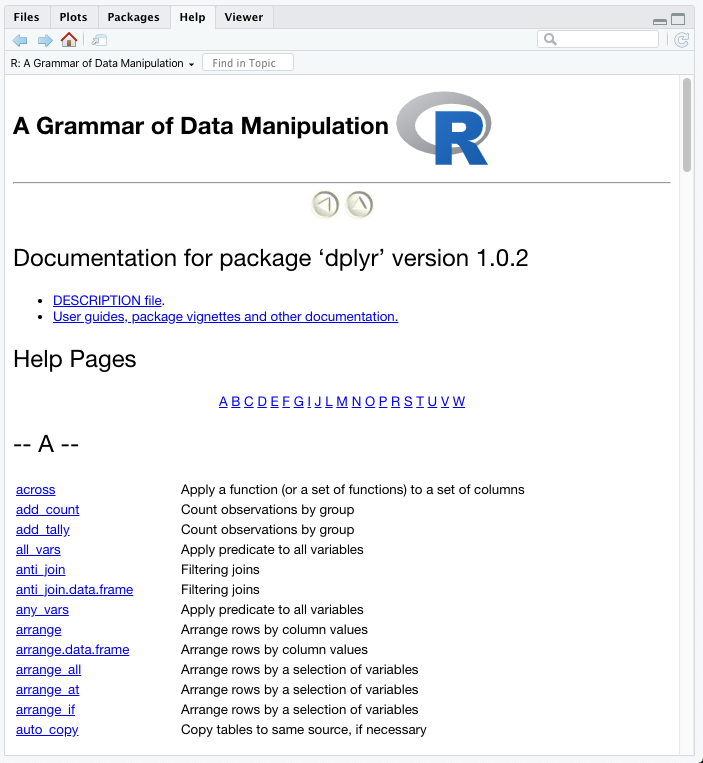
\includegraphics[width=0.6\linewidth]{1.44_Package_Documentation} \end{center}

You can select any of these hyperlinks to view instructions for how to use a specific function from this package. Down below, I select the \textbf{mutate} function documentation.

\begin{center}\includegraphics[width=0.6\linewidth]{1.45_Select_Mutate_Documentation} \end{center}

And this will take you to the documentation page.

\begin{center}\includegraphics[width=0.6\linewidth]{1.46_Mutate_Documentation} \end{center}

As you may have noticed, the documentation also lists the function's package in the top left hand of the corner. This is useful as you look up functions later.

\begin{center}\includegraphics[width=0.6\linewidth]{1.47_Package_Reference} \end{center}

You can also use certain commands to pull up this documentation. The following will bring up a package's documentation in the Help tab.

\begin{Shaded}
\begin{Highlighting}[]
\NormalTok{  ?}\KeywordTok{dplyr}\NormalTok{()}
\end{Highlighting}
\end{Shaded}

And you can look up individual functions from the package.

\begin{Shaded}
\begin{Highlighting}[]
\NormalTok{  ?}\KeywordTok{mutate}\NormalTok{()}
\end{Highlighting}
\end{Shaded}

\hypertarget{things-to-remember-5}{%
\section{Things to Remember}\label{things-to-remember-5}}

\begin{itemize}
\tightlist
\item
  Packages are what allows you to adapt R programming to meet your needs
\item
  You can install and load packages using the \textbf{Packages} tab in RStudio or the \texttt{install.packages()} and \texttt{library()} commands
\item
  Whenever you research new functions on the internet, you will often see the package required in the top left or right hand corner
\item
  You can research packages using the \textbf{Help} tab in RStudio
\end{itemize}

\hypertarget{functions}{%
\chapter{Functions}\label{functions}}

As I said a few chapters ago, R programming runs on objects. Most object types relate to the way data is stored and how it's handled. There's one object type, though, that's unique compared to the others.

That would be the \textbf{function} object type.

R functions allow you to script out various commands to transform and analyze data. This can be as simple as taking data from a vector and outputting a data frame. Or it could be something as complicated as a machine learning algorithm!

It all depends on your own R programming goals.

\hypertarget{two-approaches-to-using-r-functions}{%
\section{Two Approaches to Using R Functions}\label{two-approaches-to-using-r-functions}}

There's two approaches that you can take with functions:

\begin{enumerate}
\def\labelenumi{\arabic{enumi}.}
\tightlist
\item
  use an existing function
\item
  write your own function
\end{enumerate}

Both methods use the same underlying structure.

The more common functions you'll use include those in the R \textbf{base} and \textbf{stats} packages. These automatically come with R. These functions perform common calculations needed for statistical programming, such as \texttt{mean()}, \texttt{sum()}, \texttt{sd()}, \texttt{lm()}, \texttt{glm()} and \texttt{confint()}.

Other ``existing'' functions can include those developed by other R programmers, which you can access by installing and loading other packages. (See the chapter on R packages for more details)

\hypertarget{why-you-should-learn-to-write-your-own-functions}{%
\section{Why You Should Learn to Write Your Own Functions}\label{why-you-should-learn-to-write-your-own-functions}}

R is flexible enough though that you can write your own functions as well. This might sound like more trouble than it's worth, but it's really not. It takes a lot of time to learn other people's functions. Not only that, you have to verify that their functions perform accurately. That's especially true for packages developed by lesser known organizations.

Sadly, not every package out there goes through rigorous quality checks and much of the documentation is poorly written. So it's easy to misunderstand how a function works and then use it incorrectly.

As a matter of fact, my professor in my machine learning class suggested creating our own scripts for some more advanced machine learning processes because existing packages didn't work in every context. This is the trade off with open source programming languages.

\hypertarget{the-components-of-an-r-function}{%
\section{The Components of an R Function}\label{the-components-of-an-r-function}}

Regardless of whether you use an existing function or write your own, both require the same components to execute: \textbf{argument} and a \textbf{value}.

These are the technical terms for it, but it might be easier to think of an argument as the \textbf{input} and the value as the \textbf{output}.

Fortunately, R documentation tells you what the required arguments are for existing functions. Simply add a question mark \texttt{?} before a function and the documentation will appear in the \textbf{Help} tab on the bottom right pane of RStudio.

\begin{center}\includegraphics[width=0.5\linewidth]{1.48_Function_Documentation} \end{center}

Try it yourself with these functions:

\begin{Shaded}
\begin{Highlighting}[]
\NormalTok{?mean}
\NormalTok{?sd}
\NormalTok{?cor}
\NormalTok{?confint}
\end{Highlighting}
\end{Shaded}

In the example of the \texttt{mean} function, we see that it requires at least an \texttt{x} value. The \textbf{Arguments} section of the documentation states that x is merely an R object.

\begin{center}\includegraphics[width=0.5\linewidth]{1.48.0_Function_Documentation} \end{center}

We can see the \textbf{Value} section gives details on the output this function will generate.

\begin{center}\includegraphics[width=0.5\linewidth]{1.49_Function_Documentation} \end{center}

\hypertarget{required-versus-non-required-arguments}{%
\section{Required versus Non-Required Arguments}\label{required-versus-non-required-arguments}}

You may have noticed in the documentation for the \texttt{mean()} function that there were two other arguments: trim and na.rm. The \texttt{mean()} function still can execute, even if you don't specify what those arguments are. The reason is that there's a \emph{default} setting already in place for them.

\begin{center}\includegraphics[width=0.5\linewidth]{1.48.1_Function_Documentation} \end{center}

Whoever created this function set the default for the \emph{trim} to \texttt{0} and the \emph{na.rm} argument to \texttt{FALSE}. That way the user only has to modify those arguments if it's necessary.

\hypertarget{when-order-matters-for-arguments}{%
\section{When Order Matters for Arguments}\label{when-order-matters-for-arguments}}

If you execute \texttt{?lm} in your console, you'll see the linear model function has argument options for \emph{formula, data, subset, weights}, etc. That means we could execute the model using our Bond data as \texttt{lm(gross\textasciitilde{}actor,bond)}. Even though we don't specify the arguments, R will execute this function because the formula argument (\texttt{gross\textasciitilde{}actor}) and the data argument (\texttt{bond}) are placed in the correct order.

You can see this order in the documentation:

\begin{center}\includegraphics[width=0.5\linewidth]{1.50_Function_Documentation} \end{center}

If we tried this backwards, it wouldn't work. Executing \texttt{lm(bond,gross\textasciitilde{}actor)} in your console would throw up an error. However, if we specify the arguments with an equal \texttt{=} sign, it will execute. That would look like this: \texttt{lm(data=bond,formula=gross\textasciitilde{}actor)}.

\hypertarget{how-to-write-your-own-function}{%
\section{How to Write Your Own Function}\label{how-to-write-your-own-function}}

As you may have noticed, existing R functions require at least one argument (with the option for more) and typically displays at least one values as an output. If you write your own functions, they'll need the same thing.

According to R's own base documentation, a function is defined by an assignment, such as:

\begin{Shaded}
\begin{Highlighting}[]
\NormalTok{name <-}\StringTok{ }\ControlFlowTok{function}\NormalTok{(arg_}\DecValTok{1}\NormalTok{, arg_}\DecValTok{2}\NormalTok{, …) expression}
\end{Highlighting}
\end{Shaded}

We're going to follow this convention and create several functions, with each one becoming more and more complex.

Our end goal will be to create a function that:

\begin{enumerate}
\def\labelenumi{\arabic{enumi}.}
\tightlist
\item
  takes a data set
\item
  groups data based on a single categorical variable
\item
  calculates the mean and standard deviation of a continuous variable
\end{enumerate}

But we'll start with a simpler version of this first.

Before we begin though, go ahead and reload James Bond data set, as we'll use it in our examples later.

\begin{Shaded}
\begin{Highlighting}[]
\NormalTok{bond <-}\StringTok{ }\KeywordTok{read.csv}\NormalTok{(}\StringTok{"https://raw.githubusercontent.com/taylorrodgers/bond/main/bond.csv"}\NormalTok{)}
\end{Highlighting}
\end{Shaded}

Our first function will calculate standard deviation for a continuous variable. This function actually exists already (\texttt{?sd}), but we want to become familiar with something simple before moving on to something that's more complicated.

First, we'll need a name for the function and any arguments we know will need to be passed through. We know it'll require a data frame and a field to calculate standard deviation. I call those \texttt{data} and \texttt{field}, respectively. I name the function \texttt{sd.simple}.

You can see in the script below the template for a function and the new name and arguments that I replaced it with.

\begin{Shaded}
\begin{Highlighting}[]
\CommentTok{# Template  }
\NormalTok{name <-}\StringTok{ }\ControlFlowTok{function}\NormalTok{(arg_}\DecValTok{1}\NormalTok{, arg_}\DecValTok{2}\NormalTok{, …) expression }
\CommentTok{# New function}
\NormalTok{sd.simple <-}\StringTok{ }\ControlFlowTok{function}\NormalTok{(data, field) expression }
\end{Highlighting}
\end{Shaded}

Now we'll need to calculate add an \textbf{expression}. An expression is the actual script that takes your arguments and uses them to execute certain tasks. Our expression will need to use the data frame, grouping variable, and calculate standard deviation.

To start the expression part of a new function, we use the \texttt{\{\}} notations:

\begin{Shaded}
\begin{Highlighting}[]
\NormalTok{sd.simple <-}\StringTok{ }\ControlFlowTok{function}\NormalTok{(data, field) \{}
\NormalTok{\}}
\end{Highlighting}
\end{Shaded}

Next, we need the function to evaluate the data frame that's placed in the \texttt{data} argument and select the \texttt{field} that's specified. To do this, we use the same methods we used for selecting data from a data frame. (Note: when you design functions, it's important to keep in mind the type of objects that will be entered into a function.)

Now if we're selecting a field directly from the \textbf{Bond} data frame we created earlier, our script would look something like this:

\begin{Shaded}
\begin{Highlighting}[]
\NormalTok{bond[,}\StringTok{"gross"}\NormalTok{]}
\end{Highlighting}
\end{Shaded}

Since I want this function to be able to evaluate any data frame and field inputted, I simply replace certain parts of the script with the arguments. That means I replace ``bond'' with ``data'' and ``gross'' with ``field,'' which were the arguments I specified when I started writing this function. See what I mean below:

\begin{Shaded}
\begin{Highlighting}[]
\NormalTok{sd.simple <-}\StringTok{ }\ControlFlowTok{function}\NormalTok{(data,field) \{}
\NormalTok{  field <-}\StringTok{ }\NormalTok{data[,}\KeywordTok{paste}\NormalTok{(field)]}
\NormalTok{\}}
\end{Highlighting}
\end{Shaded}

Now you probably realized that I actually replaced ``gross'' with \texttt{paste(field)}. The \texttt{paste()} function is a handy little tool when it comes to writing your own R functions. It allows you to inject an argument into a filtering command. So when we later specify our \texttt{field} argument to be ``gross'', it'll simply plug that argument into the function to filter the data frame.

It probably confused you why we're assigning an object the name \textbf{field} when we've already specified that as an argument. This will be more clear later, but it's because the \textbf{field} argument is used to specify a variable within a data frame - not an existing R object. To make it easier to analyze in our next part of the function, we need to turn it into it's own object.

Next, we need to write a script to calculate standard devation. We'll use the \emph{sample standard deviation} equation, which is:

\[
 \sqrt{\frac{\sum{(X_i-\bar{X})^2}}{n-1}}
\]

And we'll plug that into our function:

\begin{Shaded}
\begin{Highlighting}[]
\NormalTok{sd.simple <-}\StringTok{ }\ControlFlowTok{function}\NormalTok{(data,field) \{}
\NormalTok{  field <-}\StringTok{ }\NormalTok{data[,}\KeywordTok{paste}\NormalTok{(field)]}
  \KeywordTok{sqrt}\NormalTok{(}\KeywordTok{sum}\NormalTok{((field }\OperatorTok{-}\StringTok{ }\KeywordTok{mean}\NormalTok{(field))}\OperatorTok{^}\DecValTok{2}\NormalTok{)}
       \OperatorTok{/}\StringTok{ }\NormalTok{(}\KeywordTok{length}\NormalTok{(field) }\OperatorTok{-}\StringTok{ }\DecValTok{1}\NormalTok{))}
\NormalTok{\}}
\end{Highlighting}
\end{Shaded}

And walla! We created our first function! To execute this function, we simply plug our arguments into the function.

\begin{Shaded}
\begin{Highlighting}[]
\KeywordTok{sd.simple}\NormalTok{(bond,}\StringTok{"gross"}\NormalTok{)}
\end{Highlighting}
\end{Shaded}

\begin{verbatim}
## [1] 214.4881
\end{verbatim}

If you notice, I put quotation marks around the field argument ``gross''. That's because that argument is used with filtering a data frame, which requires quotation marks when we filter down to a column by column name (i.e.~\texttt{data.frame{[},"column\ name"{]}}). If we were using column number, we wouldn't need to use a quotation mark (i.e.~\texttt{data.frame{[},n{]}}).

We can check our work against the existing \texttt{sd()} function already built into R to make sure we did it correctly.

\begin{Shaded}
\begin{Highlighting}[]
\KeywordTok{sd.simple}\NormalTok{(bond,}\StringTok{"gross"}\NormalTok{) }\OperatorTok{==}\StringTok{ }\KeywordTok{sd}\NormalTok{(bond[,}\StringTok{"gross"}\NormalTok{])}
\end{Highlighting}
\end{Shaded}

\begin{verbatim}
## [1] TRUE
\end{verbatim}

Looks like we got it right!

\hypertarget{writing-functions-using-control-flows}{%
\section{Writing Functions Using Control Flows}\label{writing-functions-using-control-flows}}

The truth is that you typically won't need to write short functions like this one because there's plenty of existing functions in base R that perform these kinds of calculations. The functions you'll need to write are able to evaluate large amounts of data and run calculations on subsets of said data. That's where things get tricky and where function writing is both a benefit and challenge.

That's where the \textbf{control flow} comes in handy. Some people call them ``loops,'' which I think is an easier term myself. A control flow simply repeats a calculation over and over again for certain subgroups. Even though this is easy to conceive, it's a challenge to implement it without lots of thought and planning.

There's several different types of control flows, which you can read up by executing \texttt{?Control} in your console.

The one we'll use is the \texttt{for\ (var\ in\ seq)\ expr} version. It's hard to visualize how that works, unless we provide an example. Down below I create a loop that prints each individual word in the \texttt{statement} vector until we reach the end.

\begin{Shaded}
\begin{Highlighting}[]
\NormalTok{statement <-}\StringTok{ }\KeywordTok{c}\NormalTok{(}\StringTok{"This"}\NormalTok{,}\StringTok{"book"}\NormalTok{,}\StringTok{"is"}\NormalTok{,}\StringTok{"the"}\NormalTok{,}\StringTok{"greatest"}\NormalTok{,}
               \StringTok{"book"}\NormalTok{,}\StringTok{"ever"}\NormalTok{,}\StringTok{"and"}\NormalTok{,}\StringTok{"I"}\NormalTok{,}\StringTok{"will"}\NormalTok{,}
               \StringTok{"recommend"}\NormalTok{,}\StringTok{"it"}\NormalTok{,}\StringTok{"to"}\NormalTok{,}\StringTok{"everyone"}\NormalTok{)}
\ControlFlowTok{for}\NormalTok{ (i }\ControlFlowTok{in} \DecValTok{1}\OperatorTok{:}\KeywordTok{length}\NormalTok{(statement)) \{}
  \KeywordTok{print}\NormalTok{(statement[i])}
\NormalTok{\}}
\end{Highlighting}
\end{Shaded}

\begin{verbatim}
## [1] "This"
## [1] "book"
## [1] "is"
## [1] "the"
## [1] "greatest"
## [1] "book"
## [1] "ever"
## [1] "and"
## [1] "I"
## [1] "will"
## [1] "recommend"
## [1] "it"
## [1] "to"
## [1] "everyone"
\end{verbatim}

First, I create the vector. Then I said print every \texttt{i} entry of the vector until we reach the end. Even though this is a simple example, you can see why this would be useful in larger, more complicated scripting.

\hypertarget{applying-a-control-flow-to-our-summary-stats-function}{%
\section{Applying a Control Flow to Our Summary Stats Function}\label{applying-a-control-flow-to-our-summary-stats-function}}

Now we're going to build upon our previous function with a control flow and use it to report both standard deviation and the average of a subgroup within a larger data frame. We'll demonstrate this using the \textbf{Bond} data frame and report those summary statistics for each Bond actor's net gross.

First, to make sure it's easy to visualize what we're doing, I'm going to replace our own \emph{standard deviation} script with the built-in \texttt{sd()} function. I'm also going to add the built-in \texttt{mean()} function and rename the function to ``summary.group''.

\begin{Shaded}
\begin{Highlighting}[]
\NormalTok{summary.group <-}\StringTok{ }\ControlFlowTok{function}\NormalTok{(data,field) \{}
\NormalTok{  field <-}\StringTok{ }\NormalTok{data[,}\KeywordTok{paste}\NormalTok{(field)]}
  \KeywordTok{sd}\NormalTok{(field)}
  \KeywordTok{mean}\NormalTok{(field)}
\NormalTok{\}}
\end{Highlighting}
\end{Shaded}

Next, I'm going to replace the \textbf{field} assignment with \textbf{groups} and \textbf{output}.

\begin{Shaded}
\begin{Highlighting}[]
\NormalTok{summary.group <-}\StringTok{ }\ControlFlowTok{function}\NormalTok{(data, group, field) \{}
\NormalTok{  groups <-}\StringTok{ }\KeywordTok{levels}\NormalTok{(}\KeywordTok{factor}\NormalTok{(data[,}\KeywordTok{paste}\NormalTok{(group)]))}
\NormalTok{  output <-}\StringTok{ }\KeywordTok{data.frame}\NormalTok{(}\DataTypeTok{group=}\KeywordTok{character}\NormalTok{(),}
                       \DataTypeTok{mean=}\KeywordTok{numeric}\NormalTok{(),}
                       \DataTypeTok{sd=}\KeywordTok{numeric}\NormalTok{())}
  \KeywordTok{sd}\NormalTok{(field)}
  \KeywordTok{mean}\NormalTok{(field)}
\NormalTok{\}}
\end{Highlighting}
\end{Shaded}

The \textbf{groups} object creates a short vector that specifies the groups we want to evaluate. Since we'll evaluate the actors in the Bond data frame, this would be Daniel Craig, Sean Connery, etc. It works similarly to the previous field object assignment we had.

The \textbf{output} object is an empty data frame that will populate with our summary statistics, such as mean and standard deviation, as the control flow evaluates each subgroup. We want to create an empty data frame before the control flow, otherwise the control flow will continuously overwrite itself.

Now we'll begin our control flow. Down below I add the control flow and it evaluates each individual group found at the beginning of the function:

\begin{Shaded}
\begin{Highlighting}[]
\NormalTok{summary.group <-}\StringTok{ }\ControlFlowTok{function}\NormalTok{(data,group,field) \{}
\NormalTok{  groups <-}\StringTok{ }\KeywordTok{levels}\NormalTok{(}\KeywordTok{factor}\NormalTok{(data[,}\KeywordTok{paste}\NormalTok{(group)]))}
\NormalTok{  output <-}\StringTok{ }\KeywordTok{data.frame}\NormalTok{(}\DataTypeTok{group=}\KeywordTok{character}\NormalTok{(),}
                       \DataTypeTok{mean=}\KeywordTok{numeric}\NormalTok{(),}
                       \DataTypeTok{sd=}\KeywordTok{numeric}\NormalTok{())}
  \ControlFlowTok{for}\NormalTok{(i }\ControlFlowTok{in} \DecValTok{1}\OperatorTok{:}\KeywordTok{length}\NormalTok{(groups)) \{}
    \CommentTok{#sd(field) - can't run properly yet}
    \CommentTok{#mean(field) - can't run properly yet}
\NormalTok{    \}}
\NormalTok{  \}}
\end{Highlighting}
\end{Shaded}

Now we'll want to update the output data frame with the group name, the mean, and the standard deviation:

\begin{Shaded}
\begin{Highlighting}[]
\NormalTok{summary.group <-}\StringTok{ }\ControlFlowTok{function}\NormalTok{(data,group,field) \{}
\NormalTok{  groups <-}\StringTok{ }\KeywordTok{levels}\NormalTok{(}\KeywordTok{factor}\NormalTok{(data[,}\KeywordTok{paste}\NormalTok{(group)]))}
\NormalTok{  output <-}\StringTok{ }\KeywordTok{data.frame}\NormalTok{(}\DataTypeTok{group=}\KeywordTok{character}\NormalTok{(),}
                       \DataTypeTok{mean=}\KeywordTok{numeric}\NormalTok{(),}
                       \DataTypeTok{sd=}\KeywordTok{numeric}\NormalTok{())}
  \ControlFlowTok{for}\NormalTok{(i }\ControlFlowTok{in} \DecValTok{1}\OperatorTok{:}\KeywordTok{length}\NormalTok{(groups)) \{}
\NormalTok{    subdata <-}\StringTok{ }\NormalTok{data[data[,}\KeywordTok{paste}\NormalTok{(group)]}\OperatorTok{==}\NormalTok{groups[i],}
                    \KeywordTok{paste}\NormalTok{(field)]}
\NormalTok{    output[i,}\DecValTok{1}\OperatorTok{:}\DecValTok{3}\NormalTok{] <-}\StringTok{ }\KeywordTok{data.frame}\NormalTok{(groups[i],}
                                \KeywordTok{mean}\NormalTok{(subdata),}
                                \KeywordTok{sd}\NormalTok{(subdata))}
\NormalTok{    \}}
\NormalTok{  \}}
\end{Highlighting}
\end{Shaded}

Now there was a lot added there and I should explain. The \textbf{subdata} object filters down the data to the group we want to evaluate. The \texttt{output{[}i,1:3{]}} object updates the output data frame for row \texttt{i} with the group name, the mean of the field within that group, and the standard deviation.

Now this function will run, but there's still one piece we're missing. We need to provide a \textbf{value}.

In this function, our value we want to use is the \textbf{output} object, which is the data frame containing our summary statistics. We can merely add the output reference at the end, outside the control flow:

\begin{Shaded}
\begin{Highlighting}[]
\NormalTok{summary.group <-}\StringTok{ }\ControlFlowTok{function}\NormalTok{(data,group,field) \{}
\NormalTok{  groups <-}\StringTok{ }\KeywordTok{levels}\NormalTok{(}\KeywordTok{factor}\NormalTok{(data[,}\KeywordTok{paste}\NormalTok{(group)]))}
\NormalTok{  output <-}\StringTok{ }\KeywordTok{data.frame}\NormalTok{(}\DataTypeTok{group=}\KeywordTok{character}\NormalTok{(),}
                       \DataTypeTok{mean=}\KeywordTok{numeric}\NormalTok{(),}
                       \DataTypeTok{sd=}\KeywordTok{numeric}\NormalTok{())}
  \ControlFlowTok{for}\NormalTok{(i }\ControlFlowTok{in} \DecValTok{1}\OperatorTok{:}\KeywordTok{length}\NormalTok{(groups)) \{}
\NormalTok{    subdata <-}\StringTok{ }\NormalTok{data[data[,}\KeywordTok{paste}\NormalTok{(group)]}\OperatorTok{==}\NormalTok{groups[i],}
                    \KeywordTok{paste}\NormalTok{(field)]}
\NormalTok{    output[i,}\DecValTok{1}\OperatorTok{:}\DecValTok{3}\NormalTok{] <-}\StringTok{ }\KeywordTok{data.frame}\NormalTok{(groups[i],}
                                \KeywordTok{mean}\NormalTok{(subdata),}
                                \KeywordTok{sd}\NormalTok{(subdata))}
\NormalTok{    \}}
\NormalTok{  output}
\NormalTok{  \}}
\end{Highlighting}
\end{Shaded}

If we run this function with the Bond data frame, we'll get this result:

\begin{Shaded}
\begin{Highlighting}[]
\KeywordTok{summary.group}\NormalTok{(bond,}\StringTok{"actor"}\NormalTok{,}\StringTok{"gross"}\NormalTok{)}
\end{Highlighting}
\end{Shaded}

\begin{verbatim}
##            group     mean        sd
## 1   Daniel Craig 820.3165 222.57396
## 2 George Lazenby 505.8998      <NA>
## 3 Pierce Brosnan  510.938  30.61869
## 4    Roger Moore 550.8332  177.6345
## 5   Sean Connery 724.8824 213.95672
## 6 Timothy Dalton  333.123  67.83394
\end{verbatim}

\hypertarget{breaking-down-the-function-we-just-made}{%
\section{Breaking Down the Function We Just Made}\label{breaking-down-the-function-we-just-made}}

This probably is confusing to you since you're not totally familiar with R control flows yet. It also doesn't help that you're still learning how to filter and transform the various object types.

To make it easier, I'm going to show you step-by-step how this function took the Bond data and created this output.

First, the function reviewed the group we defined and created a vector with the members of that group.

\begin{center}\includegraphics[width=0.5\linewidth]{1.52_Function_Breakdown} \end{center}

In this instance, that would include the Bond actors:

\begin{Shaded}
\begin{Highlighting}[]
\KeywordTok{levels}\NormalTok{(}\KeywordTok{factor}\NormalTok{(bond[,}\StringTok{"actor"}\NormalTok{]))}
\end{Highlighting}
\end{Shaded}

\begin{verbatim}
## [1] "Daniel Craig"   "George Lazenby" "Pierce Brosnan" "Roger Moore"   
## [5] "Sean Connery"   "Timothy Dalton"
\end{verbatim}

Second, the function created an empty data frame that will later store the actor names, their mean, and their standard deviation:

\begin{center}\includegraphics[width=0.5\linewidth]{1.53_Function_Breakdown} \end{center}

Our function then started a control flow, which will evaluate each actor's data to fill the data frame we just created:

\begin{center}\includegraphics[width=0.5\linewidth]{1.54_Function_Breakdown} \end{center}

Next, it filtered the Bond data set down to the first actor:

\begin{center}\includegraphics[width=0.5\linewidth]{1.55_Function_Breakdown} \end{center}

Really, this function filtered the Bond data set in a similar way to the code below:

\begin{Shaded}
\begin{Highlighting}[]
\NormalTok{groups <-}\StringTok{ }\KeywordTok{levels}\NormalTok{(}\KeywordTok{factor}\NormalTok{(bond[,}\StringTok{"actor"}\NormalTok{]))}
\NormalTok{bond[bond[,}\StringTok{"actor"}\NormalTok{]}\OperatorTok{==}\NormalTok{groups[}\DecValTok{1}\NormalTok{],}\StringTok{"gross"}\NormalTok{]}
\end{Highlighting}
\end{Shaded}

\begin{verbatim}
## [1] 1108.5610  880.6692  669.7895  622.2464
\end{verbatim}

The function then took the subdata and calculated our summary statistics. This populated the empty data set one by one\ldots{}

\begin{center}\includegraphics[width=0.5\linewidth]{1.56_Function_Breakdown} \end{center}

\ldots with each new row looked something like this:

\begin{verbatim}
##      groups.1. mean.subdata. sd.subdata.
## 1 Daniel Craig      820.3165     222.574
\end{verbatim}

And finally, it displayed the complete data frame once finished with the control flow!

\begin{center}\includegraphics[width=0.5\linewidth]{1.57_Function_Breakdown} \end{center}

\hypertarget{assigning-functions-outputs-a-name}{%
\section{Assigning Functions Outputs a Name}\label{assigning-functions-outputs-a-name}}

Any objects named within a function are not saved in your R environment. To save the results, you need to assign the executed function a name, like you would with any other object.

\begin{Shaded}
\begin{Highlighting}[]
\NormalTok{bond_eval <-}\StringTok{ }\KeywordTok{summary.group}\NormalTok{(bond,}\StringTok{"actor"}\NormalTok{,}\StringTok{"gross"}\NormalTok{)}
\NormalTok{bond_eval}
\end{Highlighting}
\end{Shaded}

This can apply to any existing functions.

\hypertarget{things-to-remember-6}{%
\section{Things to Remember}\label{things-to-remember-6}}

\begin{itemize}
\tightlist
\item
  Functions are the only object type that modifies other objects
\item
  Functions require an argument to execute and typically outputs a value
\item
  Packages store various previously built functions that you can utilize
\item
  You can build your own functions to suit your R programming needs
\item
  Control flows or ``loops'' are a handy way to automate data management tasks at a granular level
\end{itemize}

\hypertarget{exercises-1}{%
\section{Exercises}\label{exercises-1}}

Try to see if you can complete the following exercises. Answers are in the back of the book!

\begin{enumerate}
\def\labelenumi{\arabic{enumi}.}
\tightlist
\item
  Modify the simply standard deviation function we wrote and change it to calculate mean. Do this without using the built-in \texttt{mean} function.
\item
  Alter the \texttt{summary.group} function to include median, maximum, and minimum values.
\item
  Write a function for the \emph{Fibonacci Sequence}, which ends at a number you choose. You'll need to use a control flow to accomplish this and a default value for the end of the sequence. (Hint: You won't use the \texttt{for(var\ in\ seq)\ expr} control flow. Execute \texttt{?Control} to use a different version.)
\end{enumerate}

\hypertarget{importdata}{%
\chapter{Importing Data into R}\label{importdata}}

There's three good ways to import data into R:

\begin{enumerate}
\def\labelenumi{\arabic{enumi}.}
\tightlist
\item
  Import a raw data file (.csv, .xlsx, .tsv, etc.)
\item
  Connect to a database (SQL Server, AWS, etc.)
\item
  Connect to an API (Google Analytics, Census Bureau, etc.)
\end{enumerate}

Students and researchers will use the first option the most. That's because your data sets are usually smaller and don't require a database. You can both write a command or use the RStudio user interface to import raw data files.

The second option is what you'll use while working for a large organization. Most data is stored in a large database that you can access. If you work with a SQL database, you're in luck. You can access your database directly with RStudio! Although it does require some setup.

The third option involves connecting to an \emph{application programming interface} (API). That's a fancy way of saying you connect to an online application. Typically, you'll download existing packages that make this easier. That's not always true though. Sometimes you'll be stuck writing your own code to access an API and you may wonder if it's simply better to download the raw data files to import.

\hypertarget{how-to-import-a-raw-data-file-the-easy-way}{%
\section{How to Import a Raw Data File the Easy Way}\label{how-to-import-a-raw-data-file-the-easy-way}}

RStudio makes routine steps like raw data import easy. In the top right pane, you'll see an \textbf{Import Dataset} button. Click that.

\begin{center}\includegraphics[width=0.5\linewidth]{1.58_Import_Raw_Data} \end{center}

You should get a menu that looks like this:

\begin{center}\includegraphics[width=0.5\linewidth]{1.58.1_Dropdown} \end{center}

For the following example, we'll select ``From Text (readr)\ldots{}''. This allows us to import .csv, .txt, and other text files. Importing a SAS data file isn't all that different from importing a CSV file.

Click on ``From Text(readr)\ldots{}'' and you should see this screen:

\begin{center}\includegraphics[width=0.75\linewidth]{1.59_Import_Raw_Data_Screen} \end{center}

To get started, we first need to provide a file path or a URL in the top search bar. (Just use any raw data file on your computer or go to Kaggle.com to find one.)

You can select ``Browse\ldots{}'' to find a specific file on your computer.

Down below, you'll see I selected a .tsv file. As you can see, the data doesn't look right.

\begin{center}\includegraphics[width=0.75\linewidth]{1.60_Funky_Data} \end{center}

That's because the RStudio's default setting for raw data import assumes the data is \emph{comma-delimited}. We need to change the \textbf{Delimator:} option to ``Tab.''

\begin{center}\includegraphics[width=0.75\linewidth]{1.61_Change_Tab} \end{center}

The data should look like this now:

\begin{center}\includegraphics[width=0.75\linewidth]{1.62_NonFunky_Data} \end{center}

Before you hit \textbf{Import} in the bottom right-hand corner of the window, look at what RStudio produced in the box above it.

\begin{center}\includegraphics[width=0.6\linewidth]{1.63_NewCode} \end{center}

As you can see, RStudio writes the script you'll use to import this data set. Selecting ``import'' will run this script afterwards.

Go ahead and hit import now. You'll then see your data set appear as a data frame in the environment tab:

\begin{center}\includegraphics[width=0.6\linewidth]{1.64_New_Data_Frame} \end{center}

Congrats! You successfully imported a raw data file. You can follow similar steps for Excel, SAS, STATA, and other data file types!

\hypertarget{import-a-raw-data-file-the-hard-way}{%
\section{Import a Raw Data File the Hard Way}\label{import-a-raw-data-file-the-hard-way}}

In the last section, I actually provided a clue on how to import raw data the ``hard'' way. If you remember, I showed how using RStudio's built-in \textbf{Import Dataset} option will write the script that R will use to execute and import data:

\begin{center}\includegraphics[width=0.6\linewidth]{1.63_NewCode} \end{center}

The hard way is writing that code yourself. Personally, I think that's a waste of time. I could see how some people might do it to show off how good at R programming they are, but I don't seek such recognition. I say just let the RStudio UI do it.

\hypertarget{save-import-functions}{%
\section{Save Import Functions}\label{save-import-functions}}

It is a good idea, however, to save the scripts RStudio generates whenever you need to save a document. For example, you may have a raw data set saved to a URL or a shared drive in your organization. You may also need to share your R script as a saved file with other people. In that case, you want to go ahead and save the scripts to import all relevant data.

You'll need to include that at the top of your document, so future programmers can execute it and use the same data sets in your analysis.

Here's an example of how you'll do that:

\begin{Shaded}
\begin{Highlighting}[]
\KeywordTok{library}\NormalTok{(readr)}
\NormalTok{summer_train <-}\StringTok{ }\KeywordTok{read_delim}\NormalTok{(}\StringTok{"Downloads/summer_train.tsv"}\NormalTok{, }\StringTok{"}\CharTok{\textbackslash{}t}\StringTok{"}\NormalTok{, }\DataTypeTok{escape_double =} \OtherTok{FALSE}\NormalTok{, }\DataTypeTok{trim_ws =} \OtherTok{TRUE}\NormalTok{)}
\NormalTok{summer_test <-}\StringTok{ }\KeywordTok{read_delim}\NormalTok{(}\StringTok{"Downloads/summer_test.tsv"}\NormalTok{, }\StringTok{"}\CharTok{\textbackslash{}t}\StringTok{"}\NormalTok{, }\DataTypeTok{escape_double =} \OtherTok{FALSE}\NormalTok{, }\DataTypeTok{trim_ws =} \OtherTok{TRUE}\NormalTok{)}
\NormalTok{customers_data <-}\StringTok{ }\KeywordTok{read_csv}\NormalTok{(}\StringTok{"Downloads/Wholesale customers data.csv"}\NormalTok{)}

\KeywordTok{library}\NormalTok{(haven)}
\NormalTok{kidney <-}\StringTok{ }\KeywordTok{read_sas}\NormalTok{(}\StringTok{"Downloads/kidney.sas7bdat"}\NormalTok{, }\OtherTok{NULL}\NormalTok{)}
\end{Highlighting}
\end{Shaded}

In the script above, I also made sure to load both the \texttt{readr} and \texttt{haven} package. Both are required to load the file paths below them.

\hypertarget{connect-to-a-database}{%
\section{Connect to a Database}\label{connect-to-a-database}}

To connect to a database tool, work with your RStudio admin. Ask them for key connection information, such as:

\begin{enumerate}
\def\labelenumi{\arabic{enumi}.}
\tightlist
\item
  Driver
\item
  Server URL or IP address
\item
  Database name
\item
  User name and password (if different from your typical username and password)
\item
  Port
\end{enumerate}

Typically, these are the same inputs used when signing into your organization's database management software.

You'll also need to ensure there's a driver setup on your local computer or on the network you use. I would ask that your RStudio admin to do this for you.

Once they have created the driver and you have the necessary credentials, you can connect to the database in the \textbf{Connections} tab in the upper-right pane:

\begin{center}\includegraphics[width=0.6\linewidth]{1.65_Connections} \end{center}

Once you run through this process, you'll often see the menu option generate a script that looks similar to this:

\begin{Shaded}
\begin{Highlighting}[]
\KeywordTok{library}\NormalTok{(odbc)}
\NormalTok{con <-}\StringTok{ }\KeywordTok{dbConnect}\NormalTok{(}\KeywordTok{odbc}\NormalTok{(),}
                 \DataTypeTok{Driver =} \StringTok{"SQLServer"}\NormalTok{,}
                 \DataTypeTok{Server =} \StringTok{"sqlhostname"}\NormalTok{,}
                 \DataTypeTok{Database =} \StringTok{"dbase"}\NormalTok{,}
                 \DataTypeTok{UID =} \StringTok{"username"}\NormalTok{,}
                 \DataTypeTok{PWD =}\NormalTok{ rstudioapi}\OperatorTok{::}\KeywordTok{askForPassword}\NormalTok{(}\StringTok{"Database password:"}\NormalTok{),}
                 \DataTypeTok{Port =} \DecValTok{1433}\NormalTok{)}
\end{Highlighting}
\end{Shaded}

You can then use the \texttt{dbReadTable()} function in the \texttt{DBI} package to import a table from the database into an R data frame:

\begin{Shaded}
\begin{Highlighting}[]
\NormalTok{dataset <-}\StringTok{ }\KeywordTok{dbReadTable}\NormalTok{(con,}\StringTok{"tablename"}\NormalTok{)}
\end{Highlighting}
\end{Shaded}

If you intend to share your work, I would include these connections at the top of your R script.

\hypertarget{connect-to-an-api}{%
\section{Connect to an API}\label{connect-to-an-api}}

Much like database, API connections are very tool specific. Actually, I'd say they're \emph{more} tool specific than database connections. You'll need to configure both the source tool and R to accomplish this.

Fortunately, there are R packages for the most common API connections out there. I would search something like ``R package for \emph{tool-name} API connection.'' You'll often find what you need.

If you want to get practice with an API connection, you can read my article about connecting to the US Census Bureau's API at www.taylorrodgers.com.

\hypertarget{why-api-connections-are-sometimes-overrated}{%
\section{Why API Connections Are Sometimes Overrated}\label{why-api-connections-are-sometimes-overrated}}

I think API connections are a bit overrated -- at least when it comes to R programming. The reason relates to R's strengths and weaknesses.

In my professional experience, API connections are handy for ETL processes. Typically, you need to automate ETL processes. Not only for data science, but also general data reporting and application support.

That means API connections often require a \emph{production environment} -- something R programming struggles with.

One common example relates to Google Analytics. I've worked with a few marketing firms and it's not uncommon for agencies to manage multiple websites. Even if you analyze that data as a data scientist, it's more efficient to build a database first that houses all that data in a centralized, standardized location.

R can connect to the Google Analytics API and analyze data, but it can't build production quality scripts that automate that process. Therefore, it'd be better to connect to the database that already aggregated the Google Analytics data for you.

Now this doesn't mean API connections via R are useless. There are examples I've found that are more common to researchers. One example where I think connecting to an API makes sense is accessing public databases to conduct one-time analyses. A programmer spoke at my local R User Group about assisting his wife, who was an academic researcher, pull global news data from a public database online. It made sense in that context to connect to the API via R because you wouldn't have a use for that data again in the near future.

Another example would be connecting to the US Census Bureau's API. I wrote a blog post on that some time ago. Downloading that raw data files from the US Census Bureau is a pain and the API, while also a bit overwhelming, still saves a lot of time. I don't see a scenario where it makes sense for an organization to automate data collection from the US Census Bureau, because that data isn't updated that often.

\hypertarget{things-to-remember-7}{%
\section{Things to Remember}\label{things-to-remember-7}}

\begin{itemize}
\tightlist
\item
  Import raw data through the \textbf{Import Dataset} button in the \textbf{Environment} tab in the upper-right pane
\item
  Connect to databases through the \textbf{Connections} tab in the upper-right pane
\item
  Work with your data engineering or IT team for setting up the necessary drivers and credentials for database connections
\item
  API connections are handy for large, one time analysis
\item
  Download specific packages to connect to an API
\end{itemize}

\hypertarget{answers}{%
\chapter{Answer Key}\label{answers}}

\hypertarget{chapter-3}{%
\section{Chapter 3}\label{chapter-3}}

\begin{enumerate}
\def\labelenumi{\arabic{enumi}.}
\tightlist
\item
  Filter the following vector to values greater than 2
\end{enumerate}

\begin{Shaded}
\begin{Highlighting}[]
\NormalTok{  q1 <-}\StringTok{ }\KeywordTok{seq}\NormalTok{(}\DecValTok{1}\NormalTok{,}\DecValTok{20}\NormalTok{,}\DecValTok{2}\NormalTok{)}
\NormalTok{  q1[q1 }\OperatorTok{>}\StringTok{ }\DecValTok{2}\NormalTok{]}
\end{Highlighting}
\end{Shaded}

\begin{enumerate}
\def\labelenumi{\arabic{enumi}.}
\setcounter{enumi}{1}
\tightlist
\item
  Filter the following vector to values between 20 and 30, but only for the first three entries that meet that criteria. (Hint: add \texttt{{[}n:n{]}} for the range of values after you determine which values meet that criteria)
\end{enumerate}

\begin{Shaded}
\begin{Highlighting}[]
\NormalTok{  q2 <-}\StringTok{ }\KeywordTok{round}\NormalTok{(}\KeywordTok{rnorm}\NormalTok{(}\DecValTok{20}\NormalTok{,}\DecValTok{32}\NormalTok{,}\DecValTok{7}\NormalTok{),}\DecValTok{0}\NormalTok{)}
\NormalTok{  q2 }\OperatorTok{>=}\StringTok{ }\DecValTok{20} \OperatorTok{&}\StringTok{ }\NormalTok{q2 }\OperatorTok{<=}\StringTok{ }\DecValTok{30}
\NormalTok{  q2[q2 }\OperatorTok{>=}\StringTok{ }\DecValTok{20} \OperatorTok{&}\StringTok{ }\NormalTok{q2 }\OperatorTok{<=}\StringTok{ }\DecValTok{30}\NormalTok{][}\DecValTok{1}\OperatorTok{:}\DecValTok{3}\NormalTok{]}
\end{Highlighting}
\end{Shaded}

\begin{enumerate}
\def\labelenumi{\arabic{enumi}.}
\setcounter{enumi}{2}
\tightlist
\item
  Multiple the following matrices together.
\end{enumerate}

\begin{Shaded}
\begin{Highlighting}[]
\NormalTok{  q3_}\DecValTok{1}\NormalTok{ <-}\StringTok{ }\KeywordTok{matrix}\NormalTok{(}\KeywordTok{round}\NormalTok{(}\KeywordTok{seq}\NormalTok{(}\DecValTok{1}\NormalTok{,}\DecValTok{40}\NormalTok{,}\FloatTok{3.27}\NormalTok{),}\DecValTok{0}\NormalTok{),}\DecValTok{3}\NormalTok{)}
\NormalTok{  q3_}\DecValTok{2}\NormalTok{ <-}\StringTok{ }\KeywordTok{matrix}\NormalTok{(}\KeywordTok{seq}\NormalTok{(}\DecValTok{1}\NormalTok{,}\DecValTok{8}\NormalTok{,}\DecValTok{1}\NormalTok{),}\DecValTok{4}\NormalTok{)}
\NormalTok{  q3_}\DecValTok{1} \OperatorTok\StringTok{ }\NormalTok{q3_}\DecValTok{2}
\end{Highlighting}
\end{Shaded}

\begin{enumerate}
\def\labelenumi{\arabic{enumi}.}
\setcounter{enumi}{3}
\tightlist
\item
  Subtract 41 from every entry in the second column of the following matrix. Replace the column with those new values.
\end{enumerate}

\begin{Shaded}
\begin{Highlighting}[]
\NormalTok{  q4 <-}\StringTok{ }\KeywordTok{matrix}\NormalTok{(}\KeywordTok{seq}\NormalTok{(}\DecValTok{1}\NormalTok{,}\DecValTok{120}\NormalTok{,}\DecValTok{4}\NormalTok{),}\DecValTok{10}\NormalTok{,}\DecValTok{3}\NormalTok{)}
\NormalTok{  q4}
\NormalTok{  q4[,}\DecValTok{2}\NormalTok{] <-}\StringTok{ }\NormalTok{q4[,}\DecValTok{2}\NormalTok{] }\OperatorTok{-}\StringTok{ }\DecValTok{41}
\NormalTok{  q4}
\end{Highlighting}
\end{Shaded}

\begin{enumerate}
\def\labelenumi{\arabic{enumi}.}
\setcounter{enumi}{4}
\tightlist
\item
  Select the second row each matrix in the following array. Subtract 5 from those rows.
\end{enumerate}

\begin{Shaded}
\begin{Highlighting}[]
\NormalTok{  q5 <-}\StringTok{ }\KeywordTok{array}\NormalTok{(}\DataTypeTok{data=}\KeywordTok{c}\NormalTok{(}\KeywordTok{matrix}\NormalTok{(}\KeywordTok{seq}\NormalTok{(}\DecValTok{1}\NormalTok{,}\DecValTok{15}\NormalTok{,}\DecValTok{1}\NormalTok{),}\DecValTok{5}\NormalTok{,}\DecValTok{3}\NormalTok{),}
                  \KeywordTok{matrix}\NormalTok{(}\KeywordTok{seq}\NormalTok{(}\DecValTok{4}\NormalTok{,}\DecValTok{60}\NormalTok{,}\DecValTok{4}\NormalTok{),}\DecValTok{5}\NormalTok{,}\DecValTok{3}\NormalTok{),}
                  \KeywordTok{matrix}\NormalTok{(}\KeywordTok{seq}\NormalTok{(}\DecValTok{2}\NormalTok{,}\DecValTok{30}\NormalTok{,}\DecValTok{2}\NormalTok{),}\DecValTok{5}\NormalTok{,}\DecValTok{3}\NormalTok{)),}
                \DataTypeTok{dim=}\KeywordTok{c}\NormalTok{(}\DecValTok{5}\NormalTok{,}\DecValTok{3}\NormalTok{,}\DecValTok{3}\NormalTok{))}
\NormalTok{  q5}
\NormalTok{  q5[}\DecValTok{2}\NormalTok{,,]}\OperatorTok{-}\DecValTok{5}
\end{Highlighting}
\end{Shaded}

\begin{enumerate}
\def\labelenumi{\arabic{enumi}.}
\setcounter{enumi}{5}
\tightlist
\item
  Filter the following data frame to Bond films starring Roger Moore.
\end{enumerate}

\begin{Shaded}
\begin{Highlighting}[]
\NormalTok{  bond[bond[}\StringTok{"actor"}\NormalTok{]}\OperatorTok{==}\StringTok{"Roger Moore"}\NormalTok{,]}
\end{Highlighting}
\end{Shaded}

\begin{enumerate}
\def\labelenumi{\arabic{enumi}.}
\setcounter{enumi}{6}
\tightlist
\item
  Filter the following data frame to Bond films starring Sean Connery made after 1966.
\end{enumerate}

\begin{Shaded}
\begin{Highlighting}[]
\NormalTok{  bond[bond[}\StringTok{"actor"}\NormalTok{]}\OperatorTok{==}\StringTok{"Sean Connery"} \OperatorTok{&}\StringTok{ }\NormalTok{bond[}\StringTok{"year"}\NormalTok{] }\OperatorTok{>}\StringTok{ }\DecValTok{1966}\NormalTok{,]}
\end{Highlighting}
\end{Shaded}

\hypertarget{chapter-5}{%
\section{Chapter 5}\label{chapter-5}}

\begin{enumerate}
\def\labelenumi{\arabic{enumi}.}
\tightlist
\item
  Modify the simply standard deviation function we wrote and change it to calculate mean. Do this without using the built-in \texttt{mean} function.
\end{enumerate}

\begin{Shaded}
\begin{Highlighting}[]
\NormalTok{  avg.simple <-}\StringTok{ }\ControlFlowTok{function}\NormalTok{(data,field) \{}
\NormalTok{    field <-}\StringTok{ }\NormalTok{data[,}\KeywordTok{paste}\NormalTok{(field)]}
    \KeywordTok{sum}\NormalTok{(field)}\OperatorTok{/}\KeywordTok{length}\NormalTok{(field)}
\NormalTok{  \}}
\end{Highlighting}
\end{Shaded}

\begin{enumerate}
\def\labelenumi{\arabic{enumi}.}
\setcounter{enumi}{1}
\tightlist
\item
  Alter the \texttt{summary.group} function to include median, minimum, and maximum values.
\end{enumerate}

\begin{Shaded}
\begin{Highlighting}[]
\NormalTok{  summary.group <-}\StringTok{ }\ControlFlowTok{function}\NormalTok{(data,group,field) \{}
\NormalTok{    groups <-}\StringTok{ }\KeywordTok{levels}\NormalTok{(}\KeywordTok{factor}\NormalTok{(data[,}\KeywordTok{paste}\NormalTok{(group)]))}
\NormalTok{    output <-}\StringTok{ }\KeywordTok{data.frame}\NormalTok{(}\DataTypeTok{group=}\KeywordTok{character}\NormalTok{(),}
                         \DataTypeTok{mean=}\KeywordTok{numeric}\NormalTok{(),}
                         \DataTypeTok{sd=}\KeywordTok{numeric}\NormalTok{(),}
                         \DataTypeTok{median=}\KeywordTok{numeric}\NormalTok{(),}
                         \DataTypeTok{minimum=}\KeywordTok{numeric}\NormalTok{(),}
                         \DataTypeTok{maximum=}\KeywordTok{numeric}\NormalTok{())}
    \ControlFlowTok{for}\NormalTok{(i }\ControlFlowTok{in} \DecValTok{1}\OperatorTok{:}\KeywordTok{length}\NormalTok{(groups)) \{}
\NormalTok{      subdata <-}\StringTok{ }\NormalTok{data[data[,}\KeywordTok{paste}\NormalTok{(group)]}\OperatorTok{==}\NormalTok{groups[i],}
                      \KeywordTok{paste}\NormalTok{(field)]}
\NormalTok{      output[i,}\DecValTok{1}\OperatorTok{:}\DecValTok{6}\NormalTok{] <-}\StringTok{ }\KeywordTok{data.frame}\NormalTok{(groups[i],}
                                  \KeywordTok{mean}\NormalTok{(subdata),}
                                  \KeywordTok{sd}\NormalTok{(subdata),}
                                  \KeywordTok{median}\NormalTok{(subdata),}
                                  \KeywordTok{min}\NormalTok{(subdata),}
                                  \KeywordTok{max}\NormalTok{(subdata))}
\NormalTok{      \}}
\NormalTok{    output}
\NormalTok{  \}}
\end{Highlighting}
\end{Shaded}

\begin{enumerate}
\def\labelenumi{\arabic{enumi}.}
\setcounter{enumi}{2}
\tightlist
\item
  Write a function for the \emph{Fibonacci Sequence}, which ends at a number you choose. You'll need to use a control flow to accomplish this and a default value for the end of the sequence. (Hint: You won't use the \texttt{for(var\ in\ seq)\ expr} control flow. Execute \texttt{?Control} to use a different version.)
  xn=xn-1 + xn-2
  0, 1, 1, 2, 3, 5, 8, 13, 21, 34, 55
\end{enumerate}

\begin{Shaded}
\begin{Highlighting}[]
\NormalTok{  fib <-}\StringTok{ }\ControlFlowTok{function}\NormalTok{(}\DataTypeTok{end=}\DecValTok{55}\NormalTok{)\{}
\NormalTok{    x <-}\StringTok{ }\KeywordTok{c}\NormalTok{(}\DecValTok{0}\NormalTok{,}\DecValTok{1}\NormalTok{)}
\NormalTok{    n <-}\StringTok{ }\KeywordTok{length}\NormalTok{(x)}
    \ControlFlowTok{while}\NormalTok{(x[n]}\OperatorTok{<}\NormalTok{end)\{}
\NormalTok{      x[n}\OperatorTok{+}\DecValTok{1}\NormalTok{] <-}\StringTok{ }\NormalTok{x[n]}\OperatorTok{+}\NormalTok{x[n}\DecValTok{-1}\NormalTok{]}
\NormalTok{      n <-}\StringTok{ }\KeywordTok{length}\NormalTok{(x)}
\NormalTok{    \}}
\NormalTok{    x}
\NormalTok{  \}}
\end{Highlighting}
\end{Shaded}

  \bibliography{book.bib,packages.bib}

\end{document}
